\clearpage
\section{Angluar analysis of $\lcp \to p K^- \pi^+$}
\label{sec:angular}

In the weak decay of a fermion to a fermion and a scalar, a forward-backward asymmetry can be observed in the distribution of the helicity angle of decay products. This asymmetry arises from the contributions of the parity-conserving and parity-violating currents, denoted as $\alpha$. The differential decay rate is expressed as
\begin{equation}\label{eq:two-body-fermion}
    \frac{\mathrm{d}\Gamma}{\mathrm{d}\cos\theta} \varpropto 1 + P\alpha\cos\theta,
\end{equation}
where $\Gamma$ is the partial width for the decay, $\theta$ is the helicity angle of fermion in the final state and $P$ is the longitudinal polarization of the initial state. One of the most important features of $\alpha$ is its quantity does not depend on the production mechanism of fermion in the initial state. For a decay of a spin-half hadron, the differential rate of polarized decay can be expanded to be
\begin{equation}\label{eq:multi-body-hadron}
    \frac{\mathrm{d}\Gamma}{\mathrm{d}\Phi} \varpropto 1 + \vec{P}\cdot\vec{h},
\end{equation}
where $\Phi$ is the Lorentz-invariant phase space for the decay, $\vec{P}$ is the polarization vector of hadron in its rest frame and $\vec{h}$ is a polarimeter vector. The length and orientation of $\vec{h}$ depends on the kinematic variables of the decay and the dependence on the decay-plane orientation can be factored out as
\begin{equation}
    \vec{h} = R(\phi, \theta, \chi)\vec{\alpha}, 
\end{equation}
where $R$ is a three-dimensional rotation matrix with $\phi$, $\theta$ and $\chi$ being the Euler angles which describe the orientation of the decay products in space, as shown in Figure~\ref{fig:polar-angle}. This dependence of $\vec{\alpha}$ on the kinematic variables is specific cto the decay reaction and needs to be determined experimentally.
\begin{figure}[H]
    \centering
    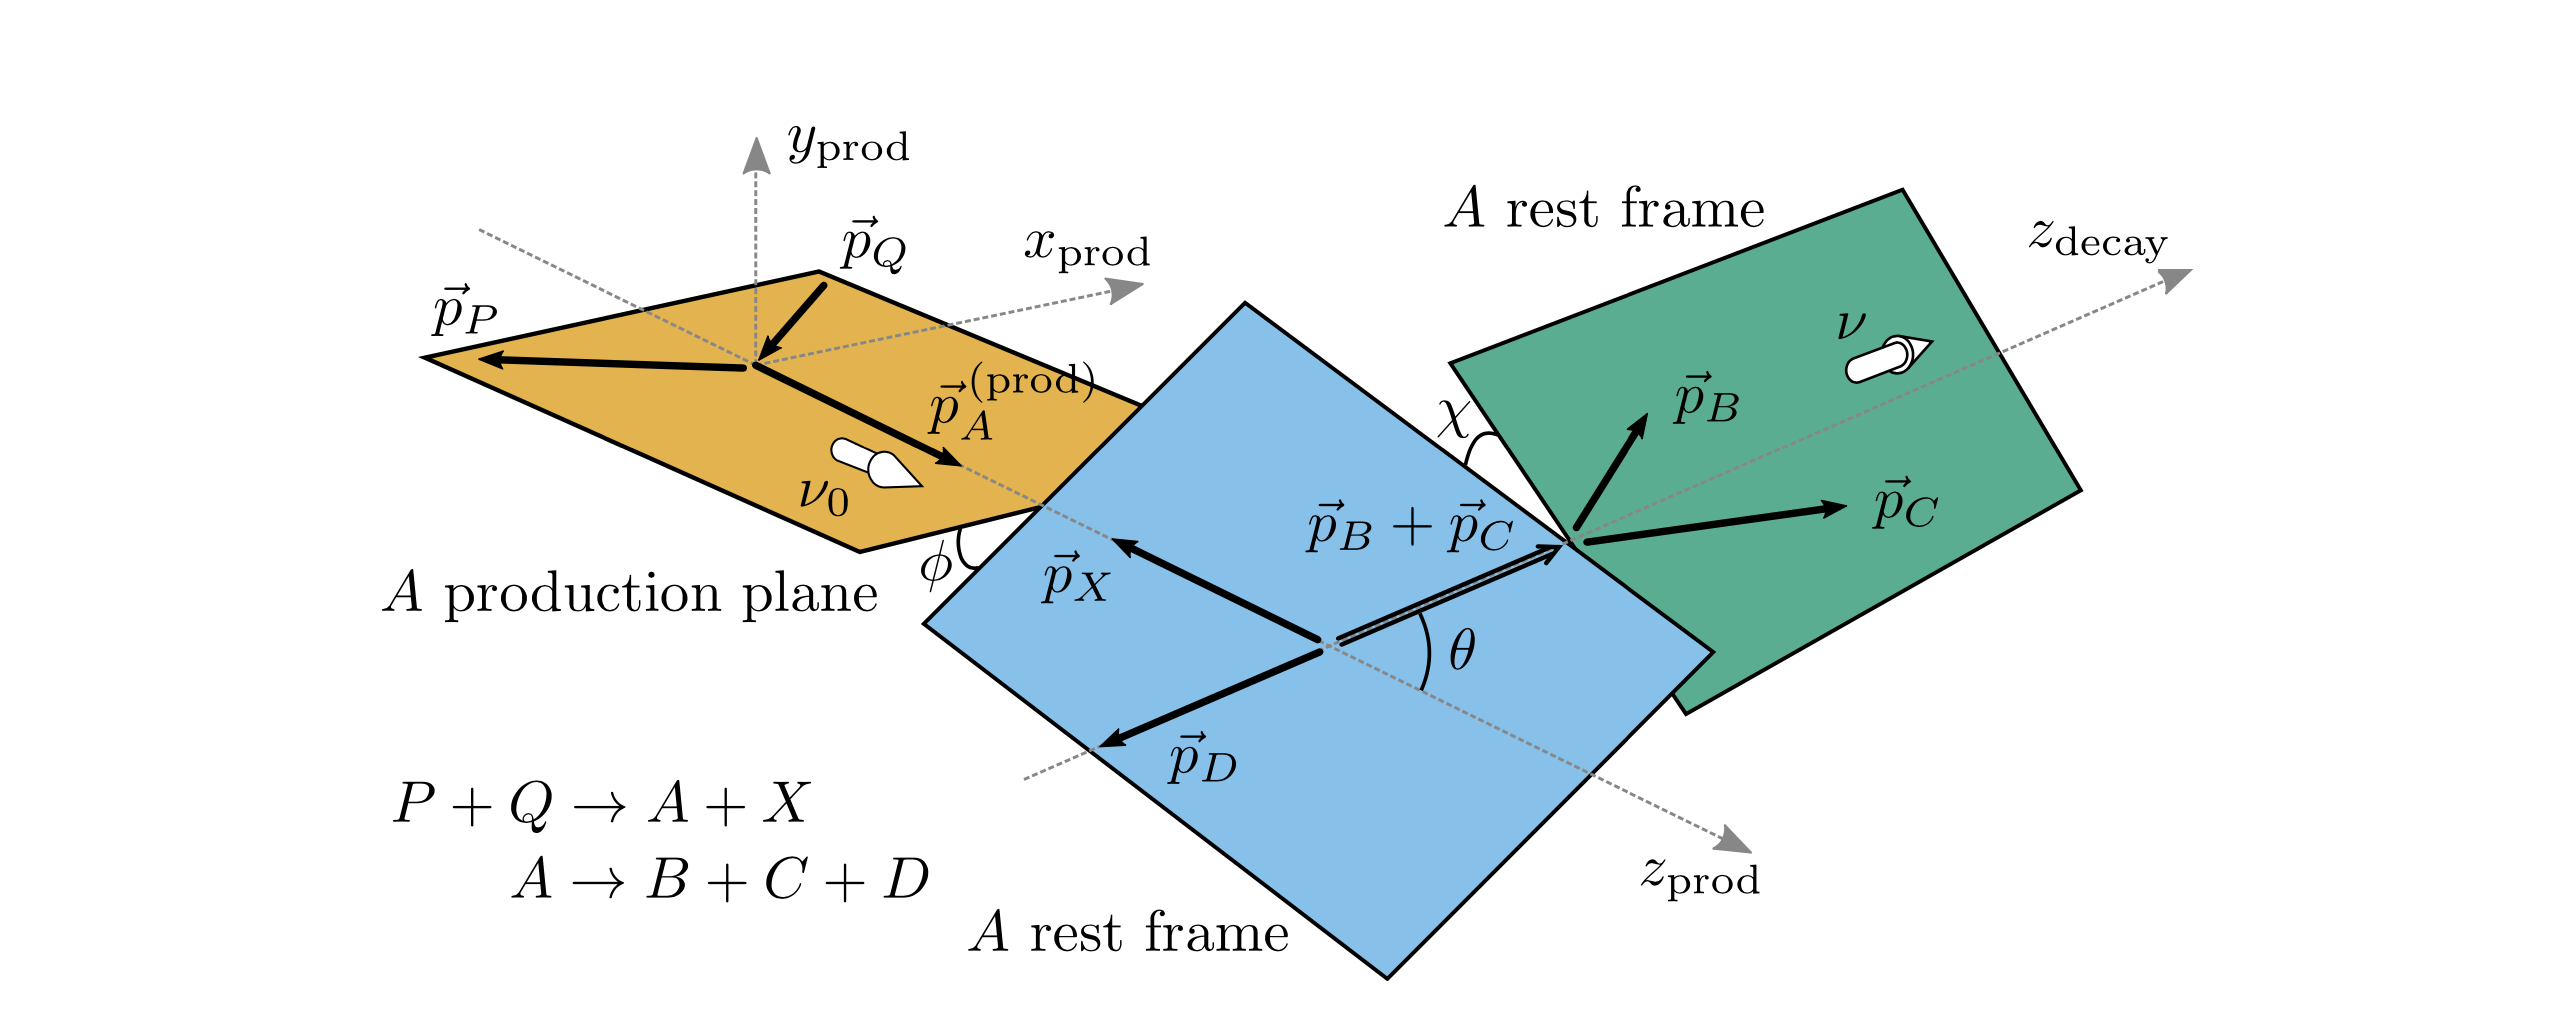
\includegraphics[width=0.90\textwidth]{figure/polarimetery/LHCb/polarimeter_angle.png}
    \caption{Definition of the decay plane orientation angles $\phi$, $\theta$ and $\chi$ related to the polarization of particle $A$, produced in the process of $P + Q \to A + X$ with $A \to B + C +D$~\cite{LHCb:2023crj}.}
    \label{fig:polar-angle}
\end{figure}

Recently, the LHCb collaboration reported a new result~\cite{LHCb:2023crj} of a model-agnostic representation using the distribution of the aligned polarimeter vector $\vec{\alpha}$ converted from the transition amplitude for the $\lcp \to p K^- \pi^+$~\cite{LHCb:2022ouv}. The components of the aligned polarimeter vector are computed on a two-dimensional grid of the Dalitz-plot variables. The expression for the differential decay rate can be written as
\begin{equation}\label{eq:lhcb-decay-rate}
    |\mathcal{M}(\phi,\theta,\chi,\kappa)|^2 = I_{0}(\kappa)(1+ \sum_{i,j}P_iR_{ij}(\theta,\phi,\chi)\alpha_j(\kappa)),
\end{equation}
where $R_{ij}(\theta,\phi,\chi)$ is a three-dimensional rotation matrix implementing the Euler transformation to a physical vector. $\vec{\alpha}(\kappa)$ denotes the model-agnostic representation for polarization dependence of the decay rate and $I_0(\kappa)$ is the total differential decay rate, where $\kappa$ represent the Dalitz-plot variables such as $M^2(pK^-)$ and $M^2(K^-\pi^+)$. The distributions of $I_0(\kappa)$ and the $\vec{\alpha}$ components are shown in Figure~\ref{fig:lhcb-results}.
\begin{figure}[H]
    \centering
    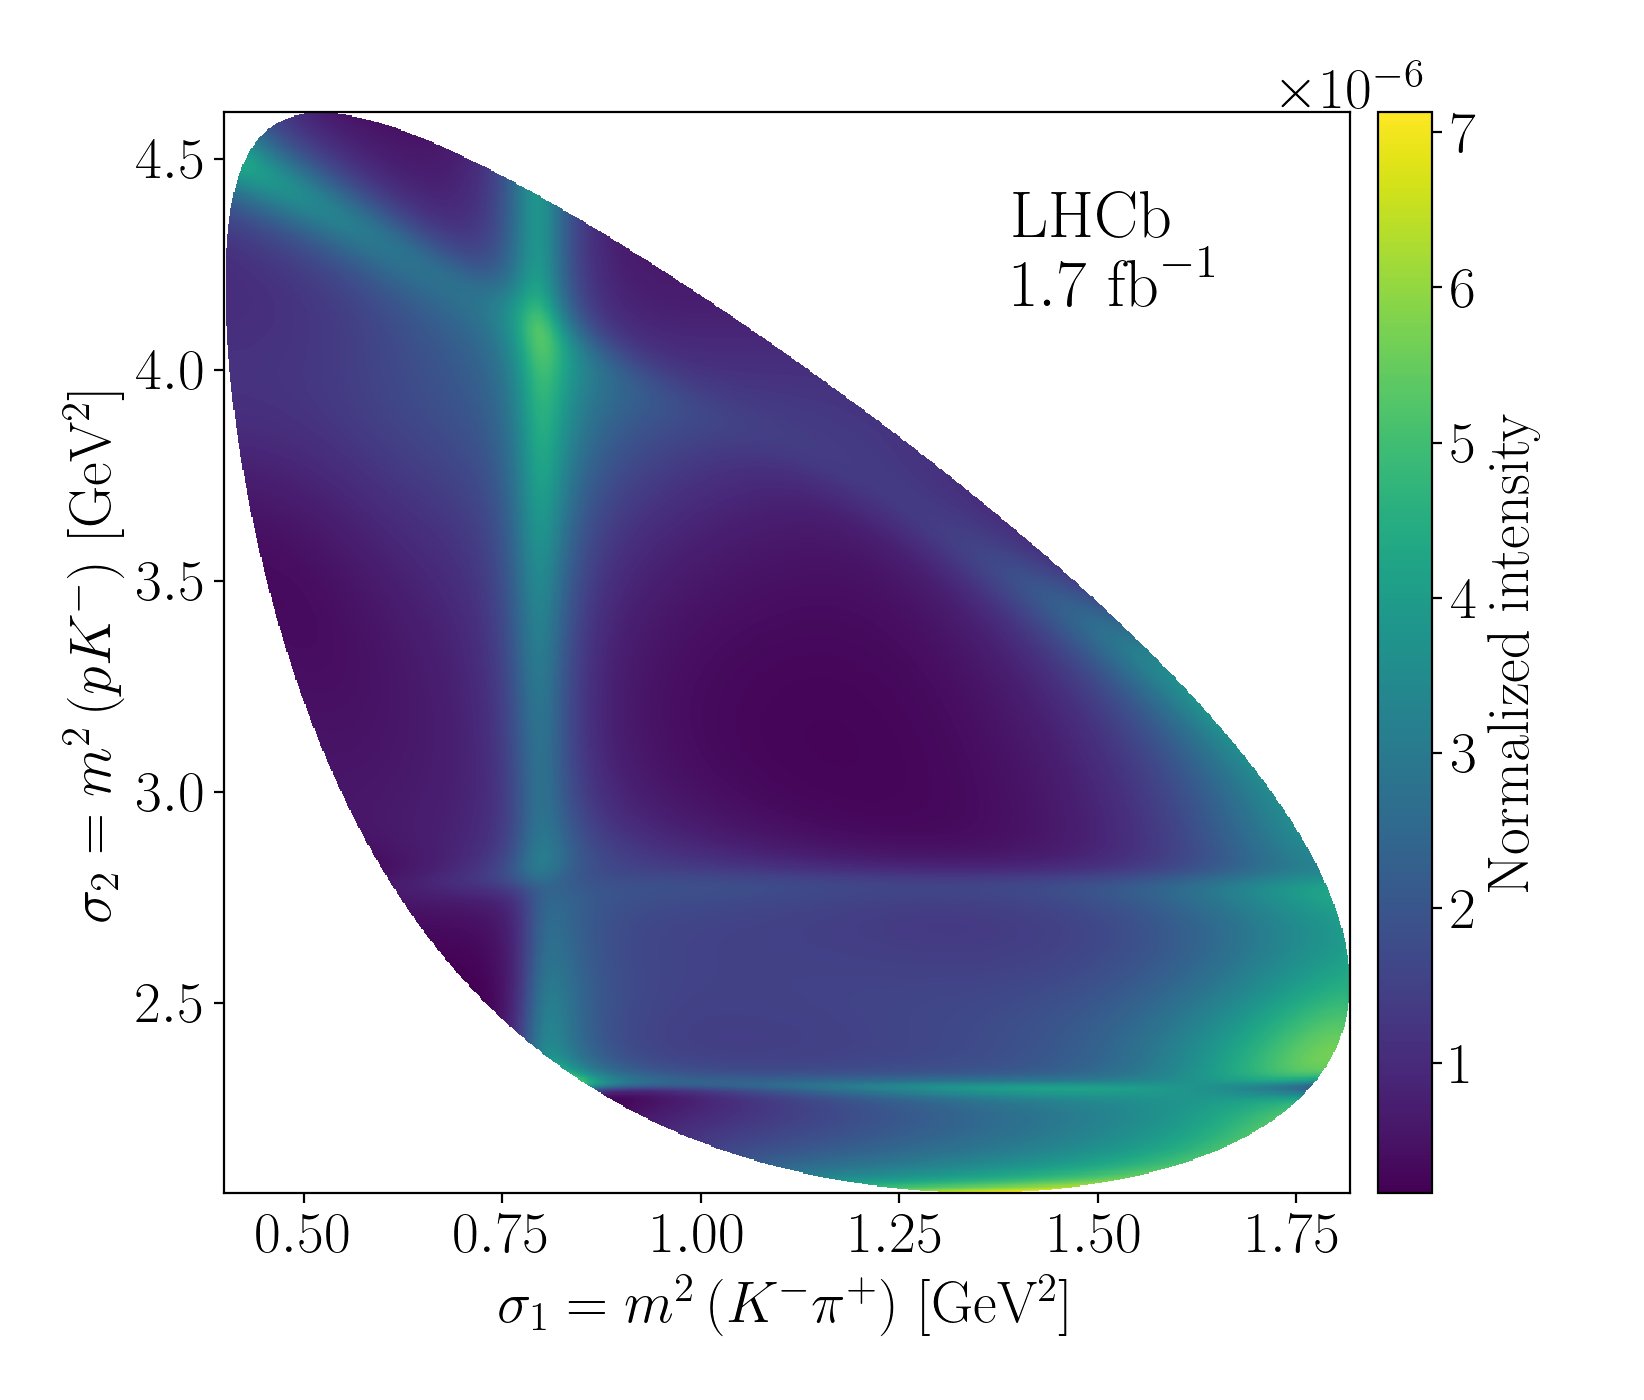
\includegraphics[width=0.45\textwidth]{figure/polarimetery/LHCb/intensity-distribution.png}
    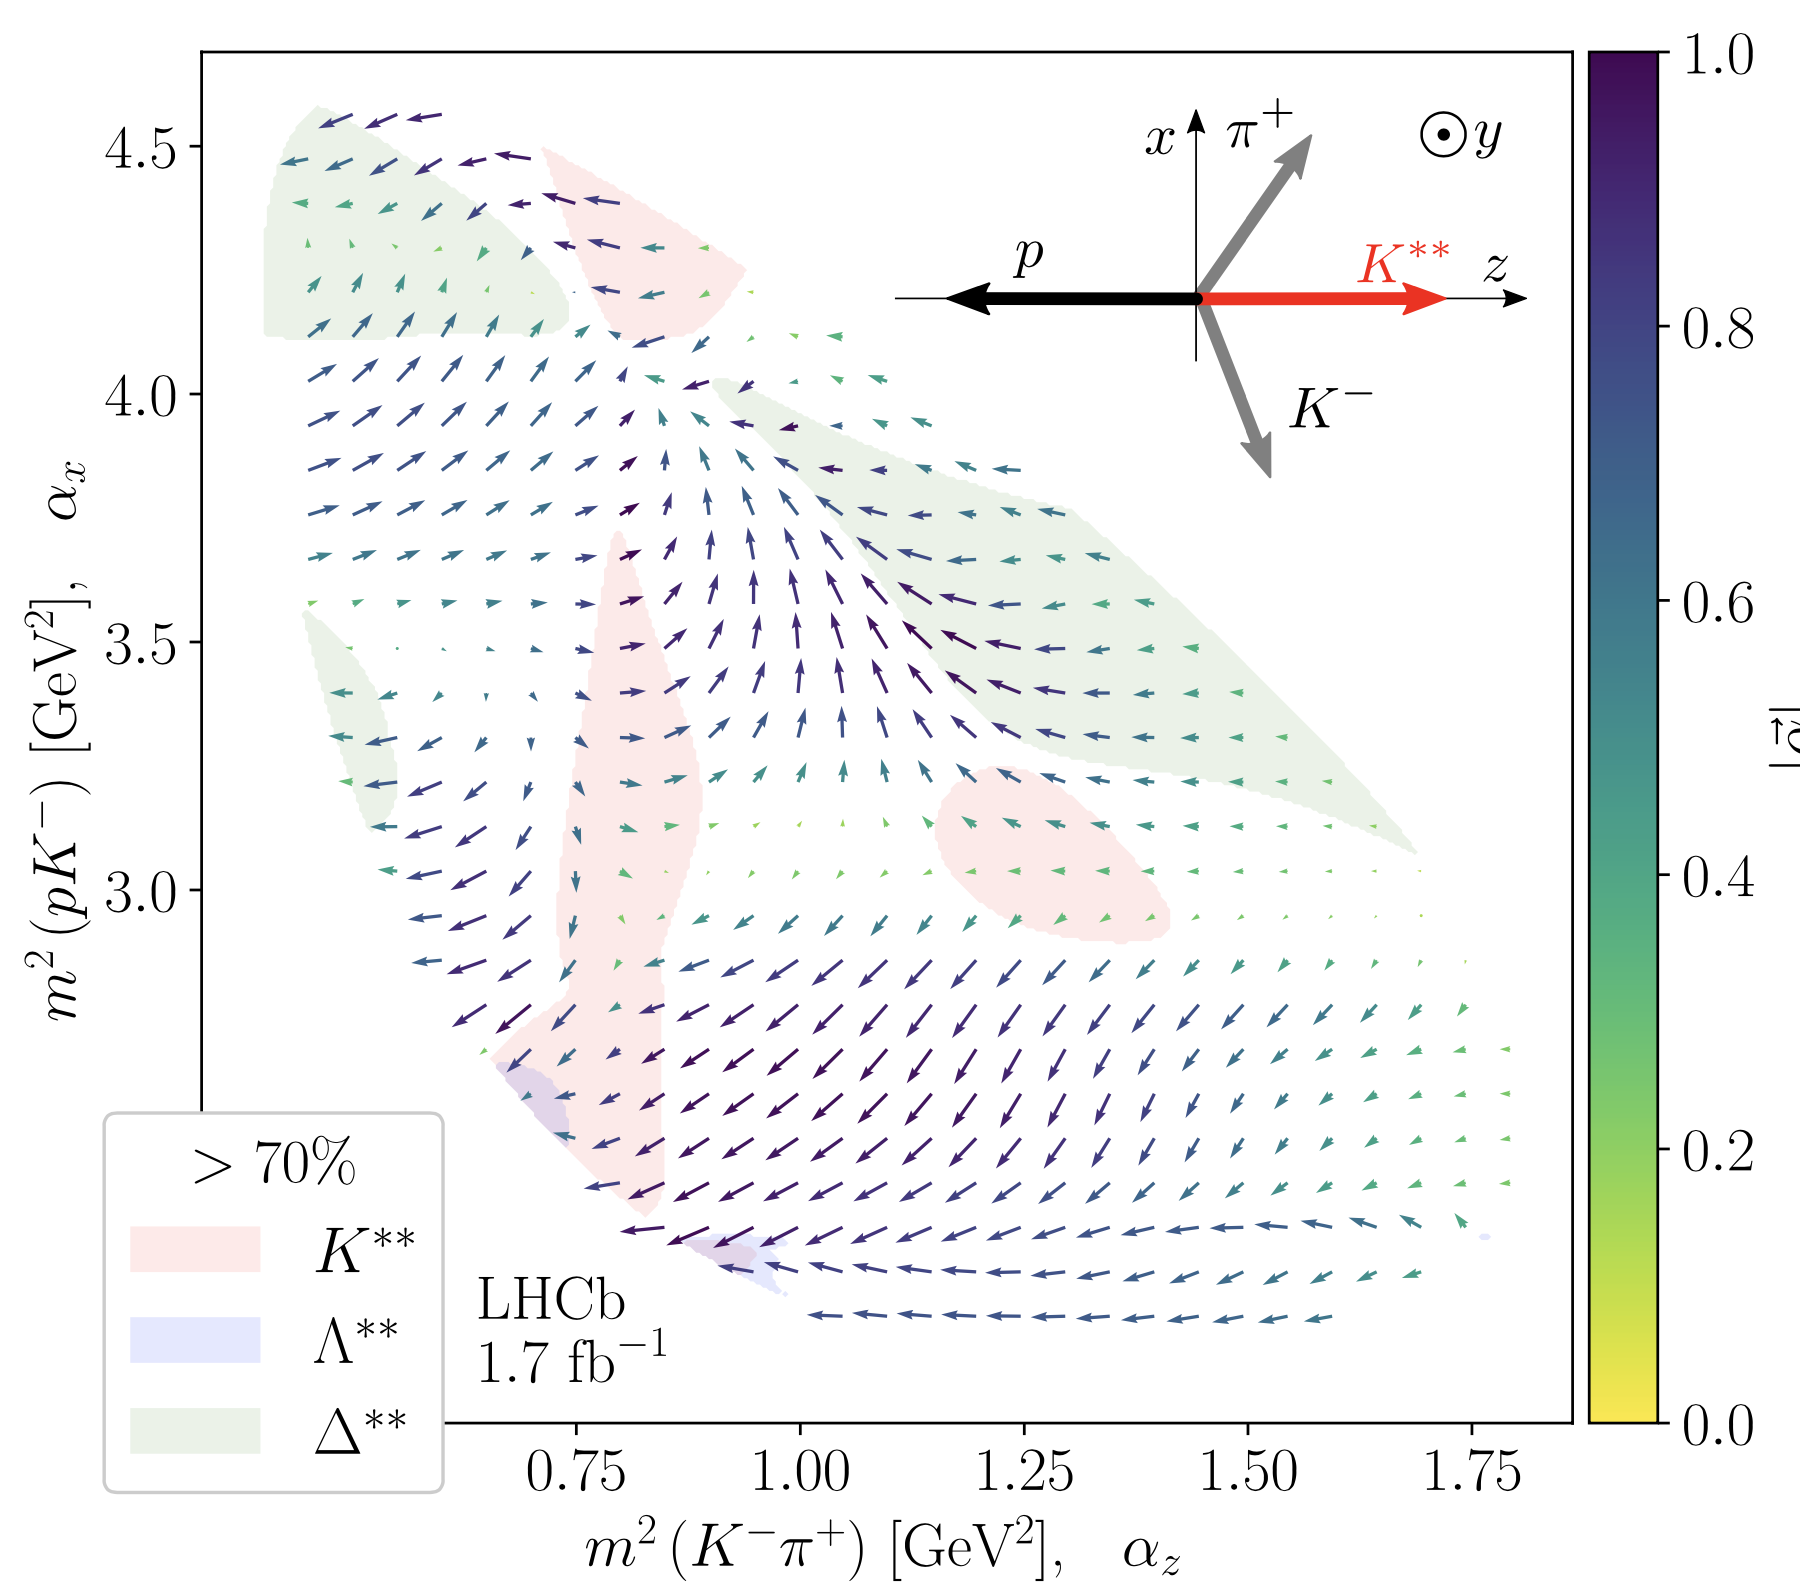
\includegraphics[width=0.45\textwidth]{figure/polarimetery/LHCb/total-polarimetry-field-watermark.png}
    \caption{Distributions of $I_0(\kappa)$ and the $\vec{\alpha}$ components in Dalitz-plot coordinates: $M^2(pK^-)$ and $M^2(K^-\pi^+)$. The sketch in the top right corner of the right figure shows the decay-plane orientation.}
    \label{fig:lhcb-results}
\end{figure}

For the $\lcp$ production in the process of $e^+e^-\to\lcp\lcm$, $\lcp$ have none-zero transverse polarization perpendicular to the production plane formed by the $z$-axis and direction of $\lcp$ in the c.m. frame. The polarization vector $\vec{P}$ in Eq.~(\ref{eq:lhcb-decay-rate}) is replaced by $P_y \varpropto \sqrt{1-\alpha_0^2}\sin\Delta_0\sin\theta_{\lcp}\cos\theta_{\lcp}$ and $P_x = P_z = 0$. Taking the unpolarized cross section $P_0 \varpropto 1 + \alpha_0\cos\theta_{\lcp}$ into account, the full angular distribution is written as
\begin{equation}\label{eq:angular-distribution}
    |\mathcal{M}(\phi,\theta,\chi,\kappa)|^2 \varpropto I_0(\kappa)(1+\alpha_0\cos\theta_{\lcp} + \sum_{j}\sqrt{1-\alpha_0^2}\sin\Delta_0\sin\theta_{\lcp}\cos\theta_{\lcp}R_{2j}(\theta, \phi, \chi)\alpha_j(\kappa)),
\end{equation}
where the reduced rotation matrix is
\begin{equation}
R_{2j}(\theta,\phi,\chi) = (\sin\chi\cos\phi+\sin\phi\cos\chi\cos\theta, -\sin\chi\sin\phi\cos\theta+\cos\chi\cos\phi, \sin\phi\sin\theta).
\end{equation}
For each event, we use the four-momentum information of the particles in the final state to calculate the three helicity angles ($\theta,\phi, \chi$) following the definitions as shown in Figure~\ref{fig:polar-angle}. The information of total differential decay rate $I_0$ and three components of the aligned polarimeter vector $\vec{\alpha}$ are extracted using the two Dalitz-plot variables, $M^2(pK^-)$ and $M^2(K^-\pi^+)$, from Figure~\ref{fig:lhcb-results}. The probability density function for an event to be observed is defined by
\begin{equation}\label{eq:angluar-pdf}
    P(\zeta,\eta) = \frac{\omega(\zeta, \eta)\epsilon(\zeta)}{\int\mathrm{d}\zeta\omega(\zeta,\eta)\epsilon(\zeta)},
\end{equation}
where $\zeta$ represents the variables measured by the experiments such as the helicity angles, $\eta$ is the variables to be measured, i.e. $\Delta_0$ and $\alpha_0$, $\omega(\zeta, \eta)$ is the angular distribution function Eq.~(\ref{eq:angular-distribution}), and $\epsilon(\zeta)$ is the detection efficiency. Similar to the case of partial wave analysis, the denominator in the Eq.~(\ref{eq:angluar-pdf}) is calculated using the MC integration from the PHSP signal MC samples. The joint likelihood function is constructed with the background subtraction method where the background is described by the data events in the $\mbc$ sideband region. 


The unbinned maximum-likelihood fit is performed in each energy point to evaluate the transverse polarization parameters $\alpha_0$ and $\Delta_0$. The fit results are shown in Figure~\ref{fig:fit_angular_s0}-\ref{fig:fit_angular_s12}. The obtained $\alpha_0$ and $\sin\Delta_0$ are listed in Table~\ref{tab:angular-fit}. Comparing to the results of amplitude analysis in Section~\ref{sec:pwa}, the deviations are derived by $|\mu_\mathrm{AMP} - \mu_\mathrm{Angular}|/\sqrt{\sigma_\mathrm{AMP}^2 + \sigma_\mathrm{Angular}^2}$, where $\mu$ and $\sigma$ are the central value and corresponding errors. Results from two method are in good agreement within $1\sigma$ of statistical error. The difference could be due to the different models between the LHCb and our work. These two approaches using the same data statistics which results in comparable statistical uncertainties of $\alpha_0$ and $\sin\Delta_0$. Simultaneous fit between two approaches cannot improve the precision of transverse polarization parameters.

\begin{figure}[H]\centering
    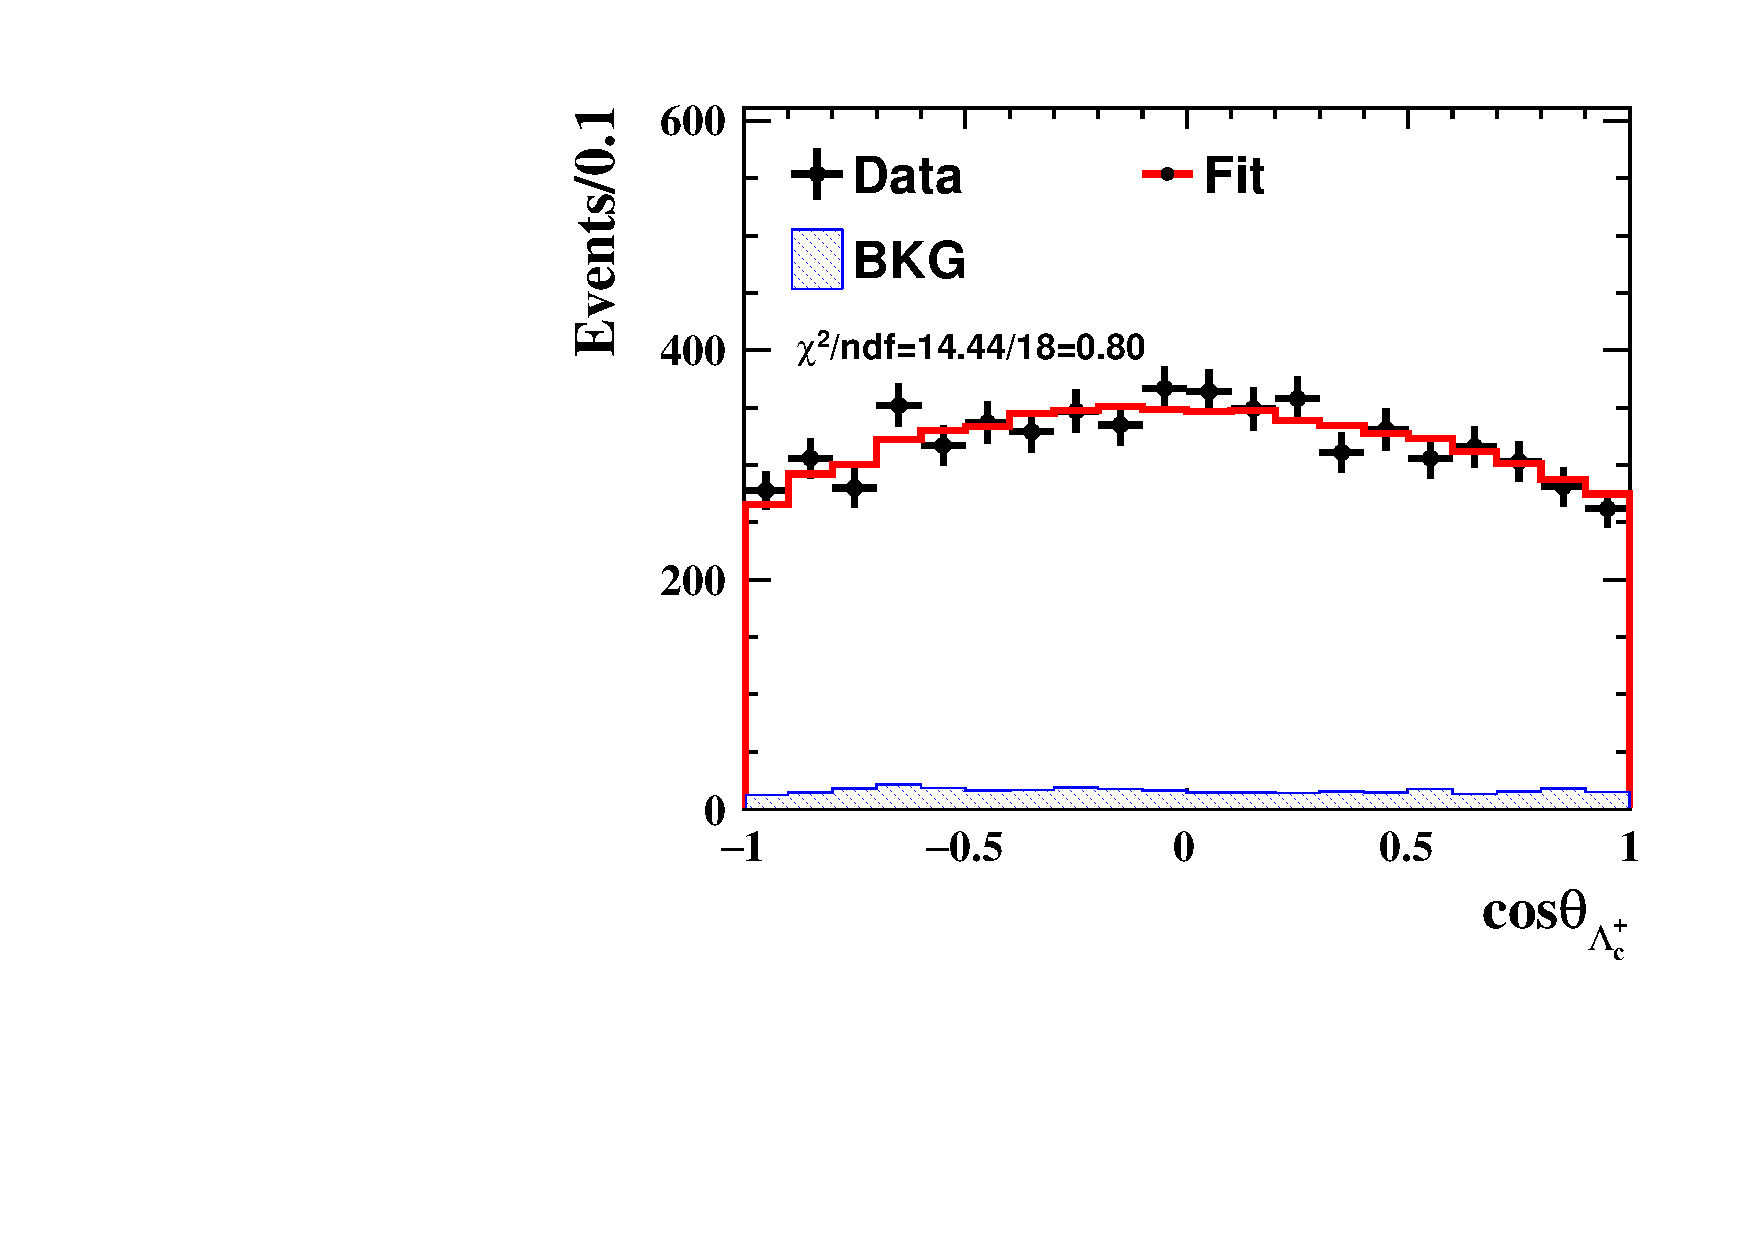
\includegraphics[width=0.24\textwidth]{figure/polarimetery/angular_plots/pkpi_4600_cos_theta0.pdf}
    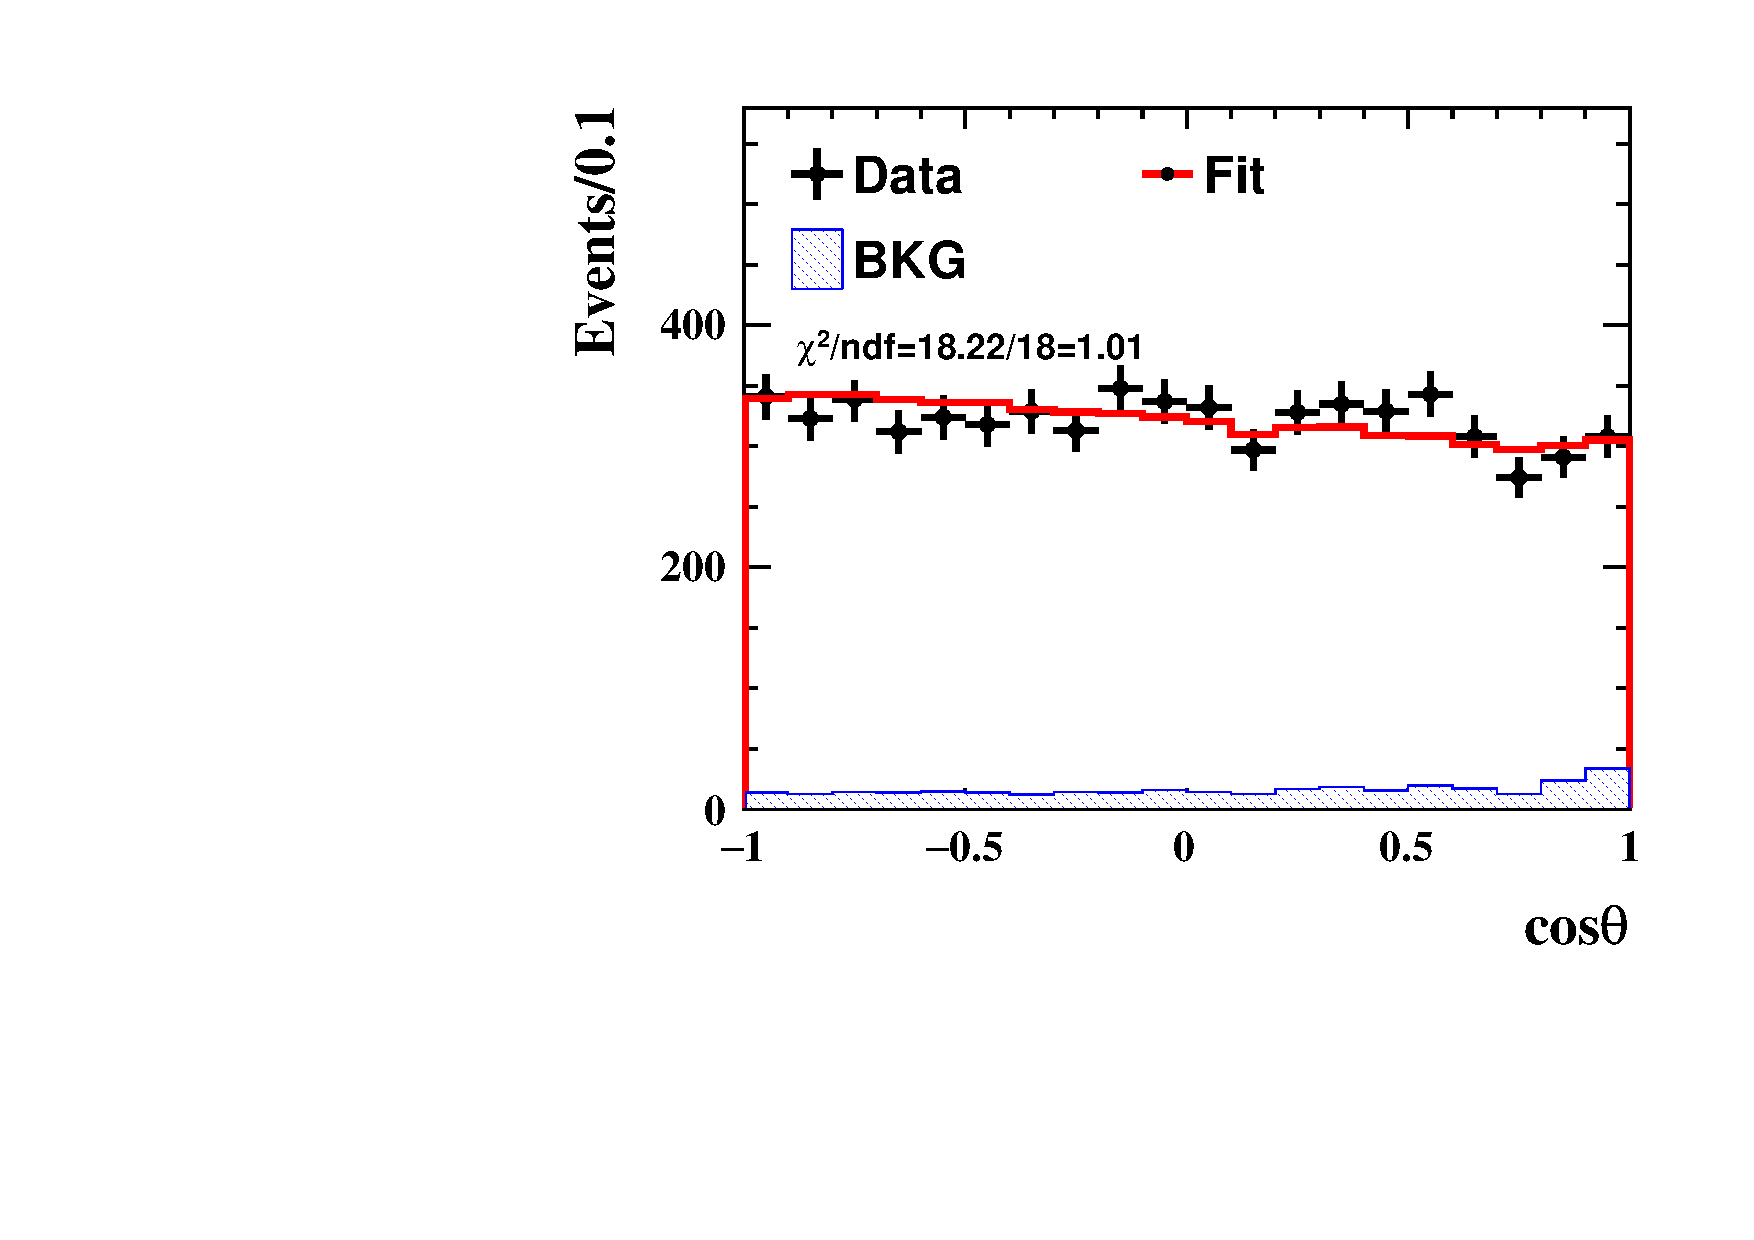
\includegraphics[width=0.24\textwidth]{figure/polarimetery/angular_plots/pkpi_4600_cos_theta1.pdf}
    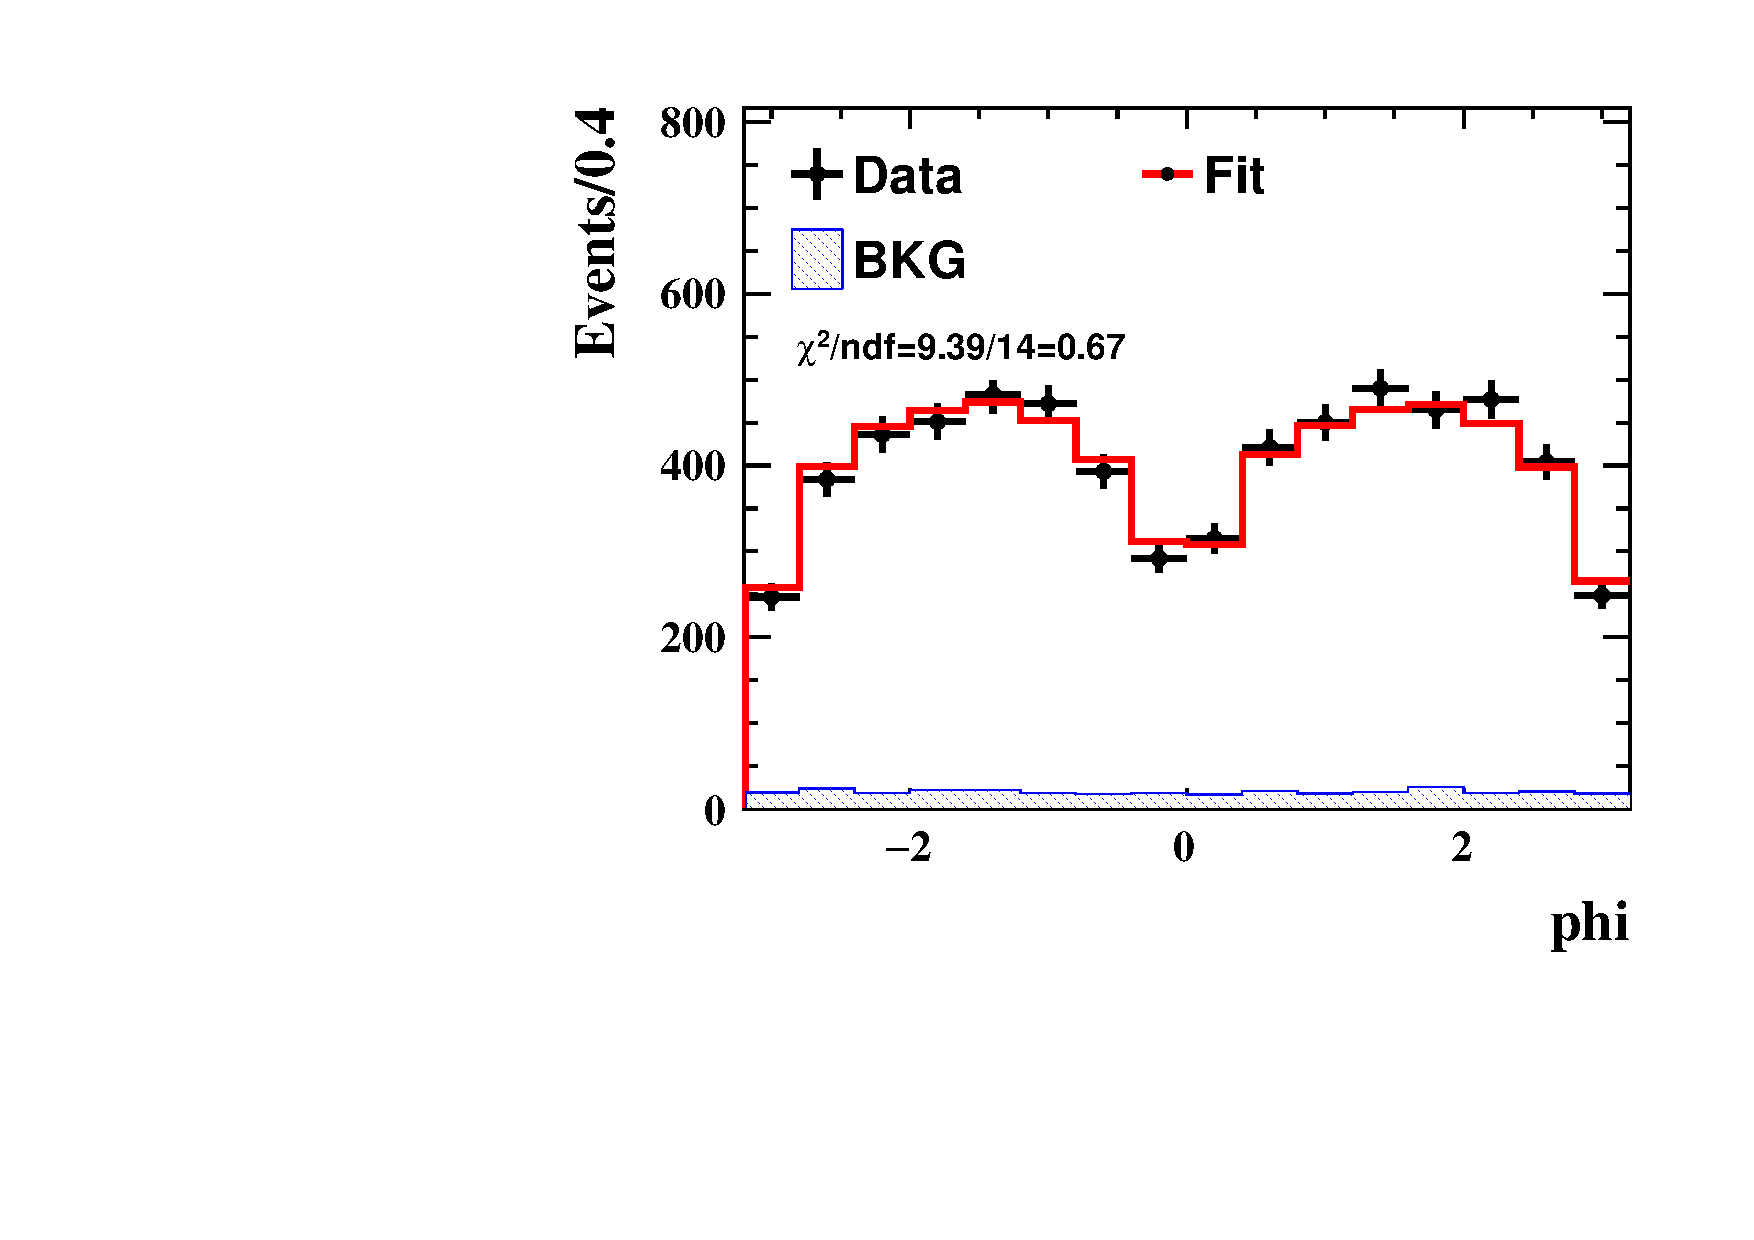
\includegraphics[width=0.24\textwidth]{figure/polarimetery/angular_plots/pkpi_4600_phi1.pdf}
    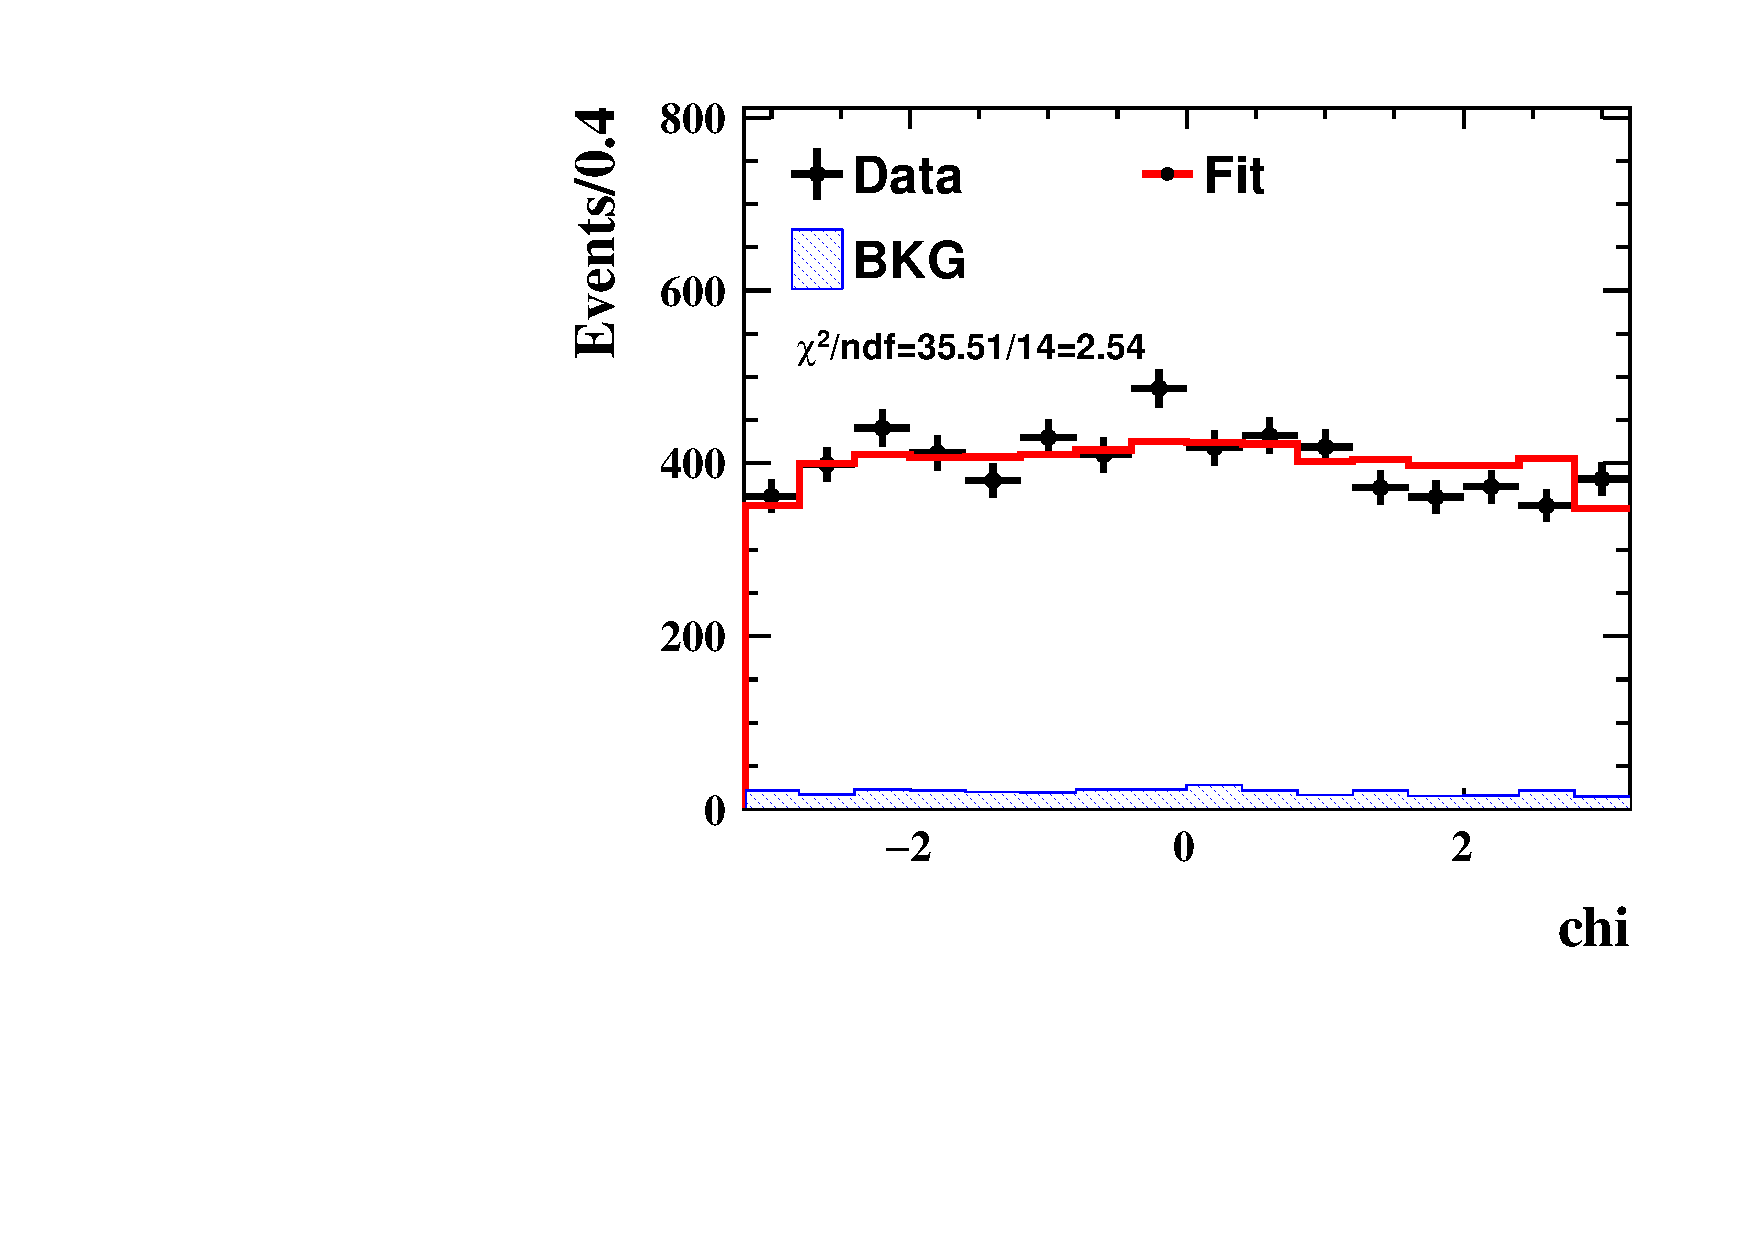
\includegraphics[width=0.24\textwidth]{figure/polarimetery/angular_plots/pkpi_4600_phi2.pdf}
    \caption{Fit results of helicity angles of $\theta_{\lcp}$, $\theta$, $\phi$ and $\chi$ at $\sqrt{s} = 4.599\gev/c^2$.}
\label{fig:fit_angular_s0}
\end{figure}

\begin{figure}[H]\centering
    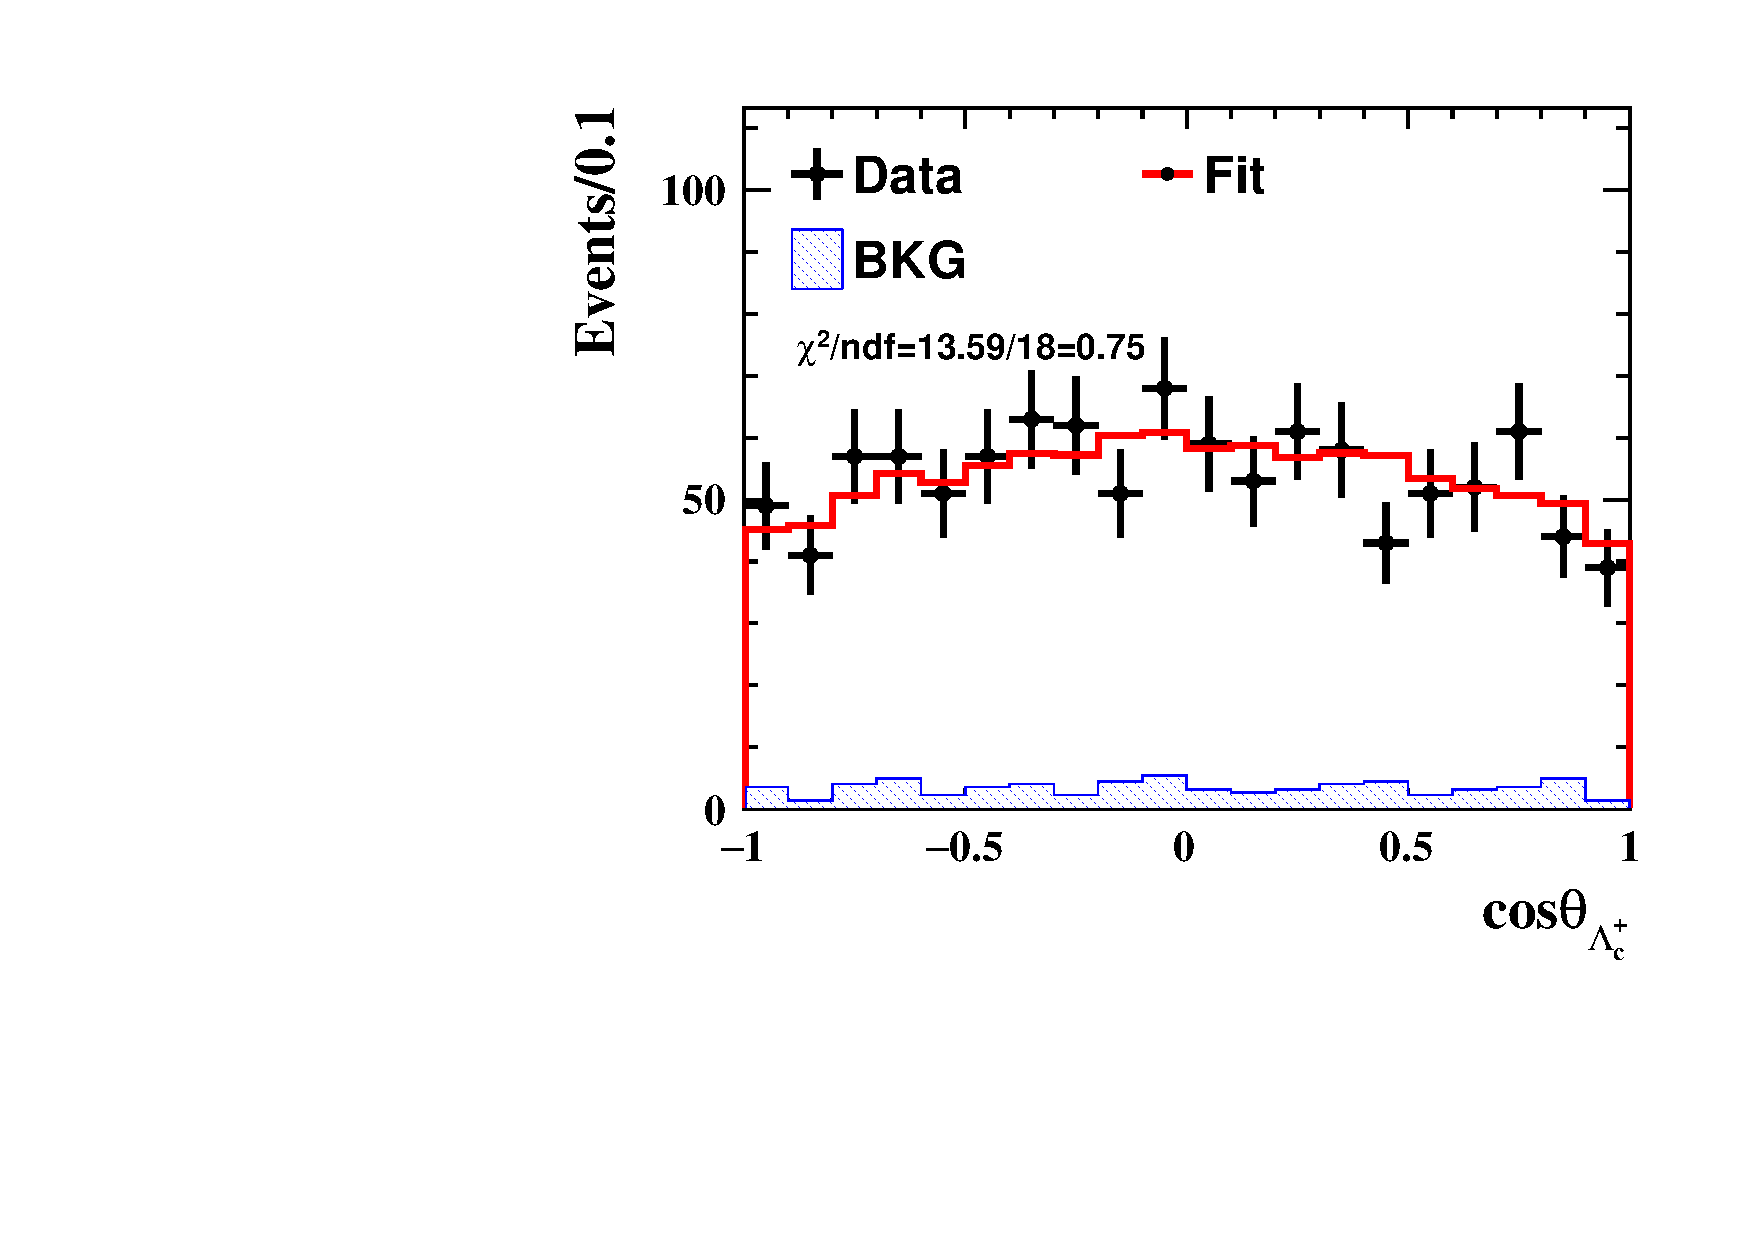
\includegraphics[width=0.24\textwidth]{figure/polarimetery/angular_plots/pkpi_4612_cos_theta0.pdf}
    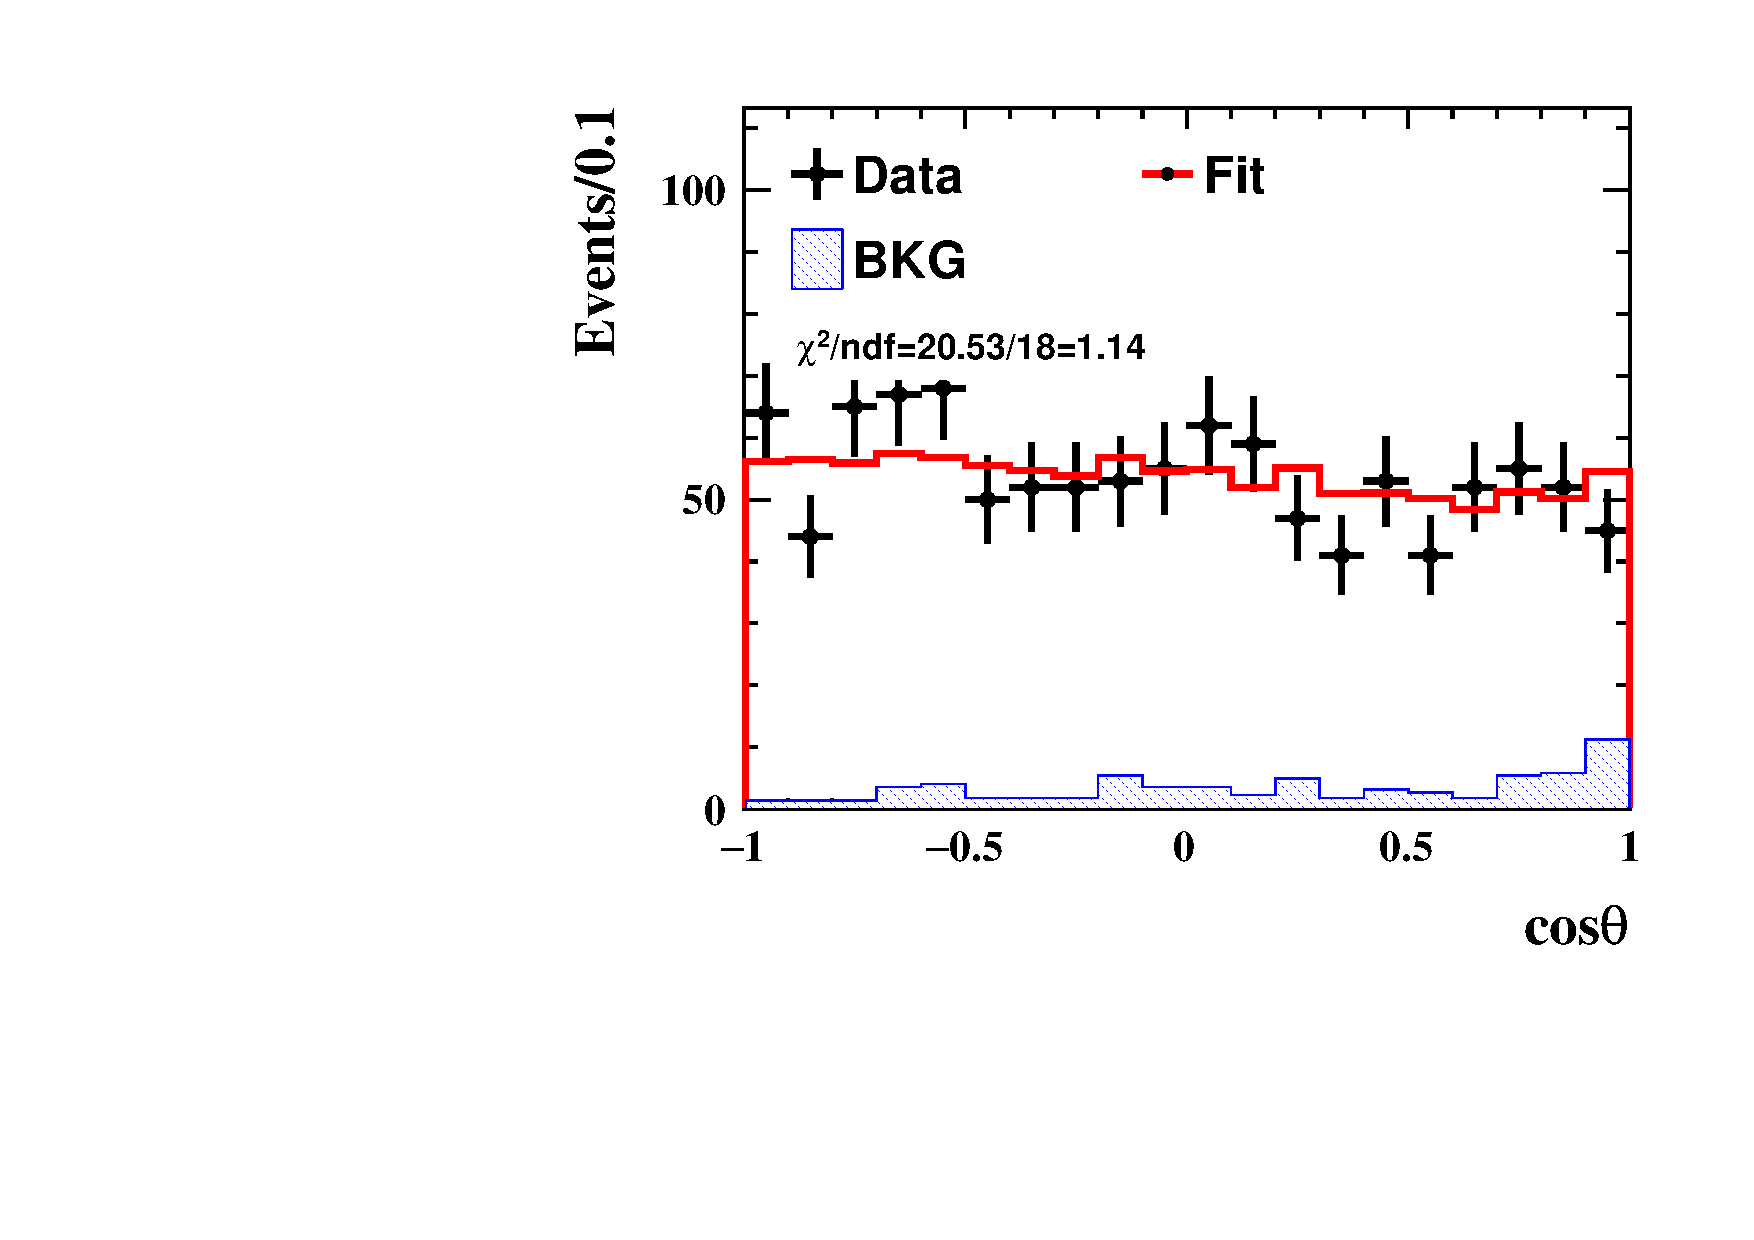
\includegraphics[width=0.24\textwidth]{figure/polarimetery/angular_plots/pkpi_4612_cos_theta1.pdf}
    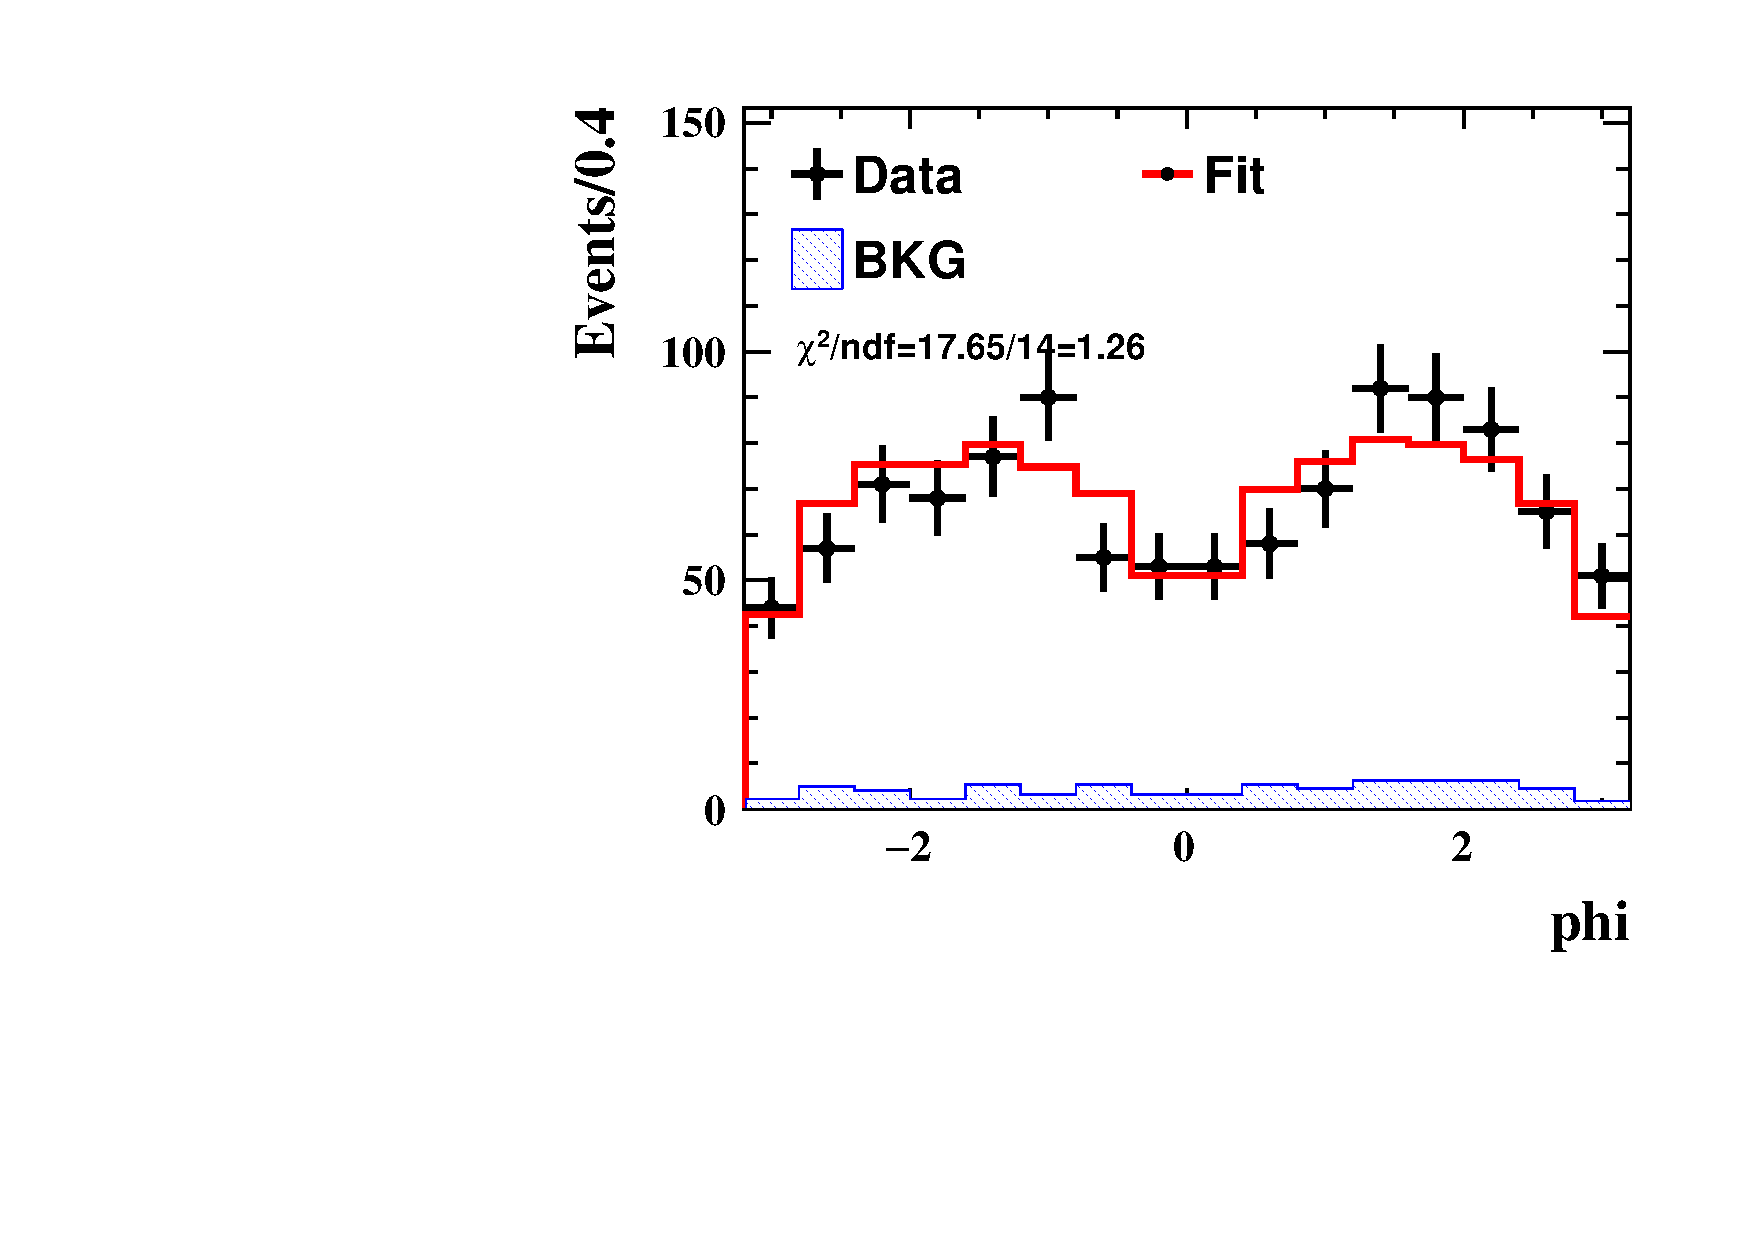
\includegraphics[width=0.24\textwidth]{figure/polarimetery/angular_plots/pkpi_4612_phi1.pdf}
    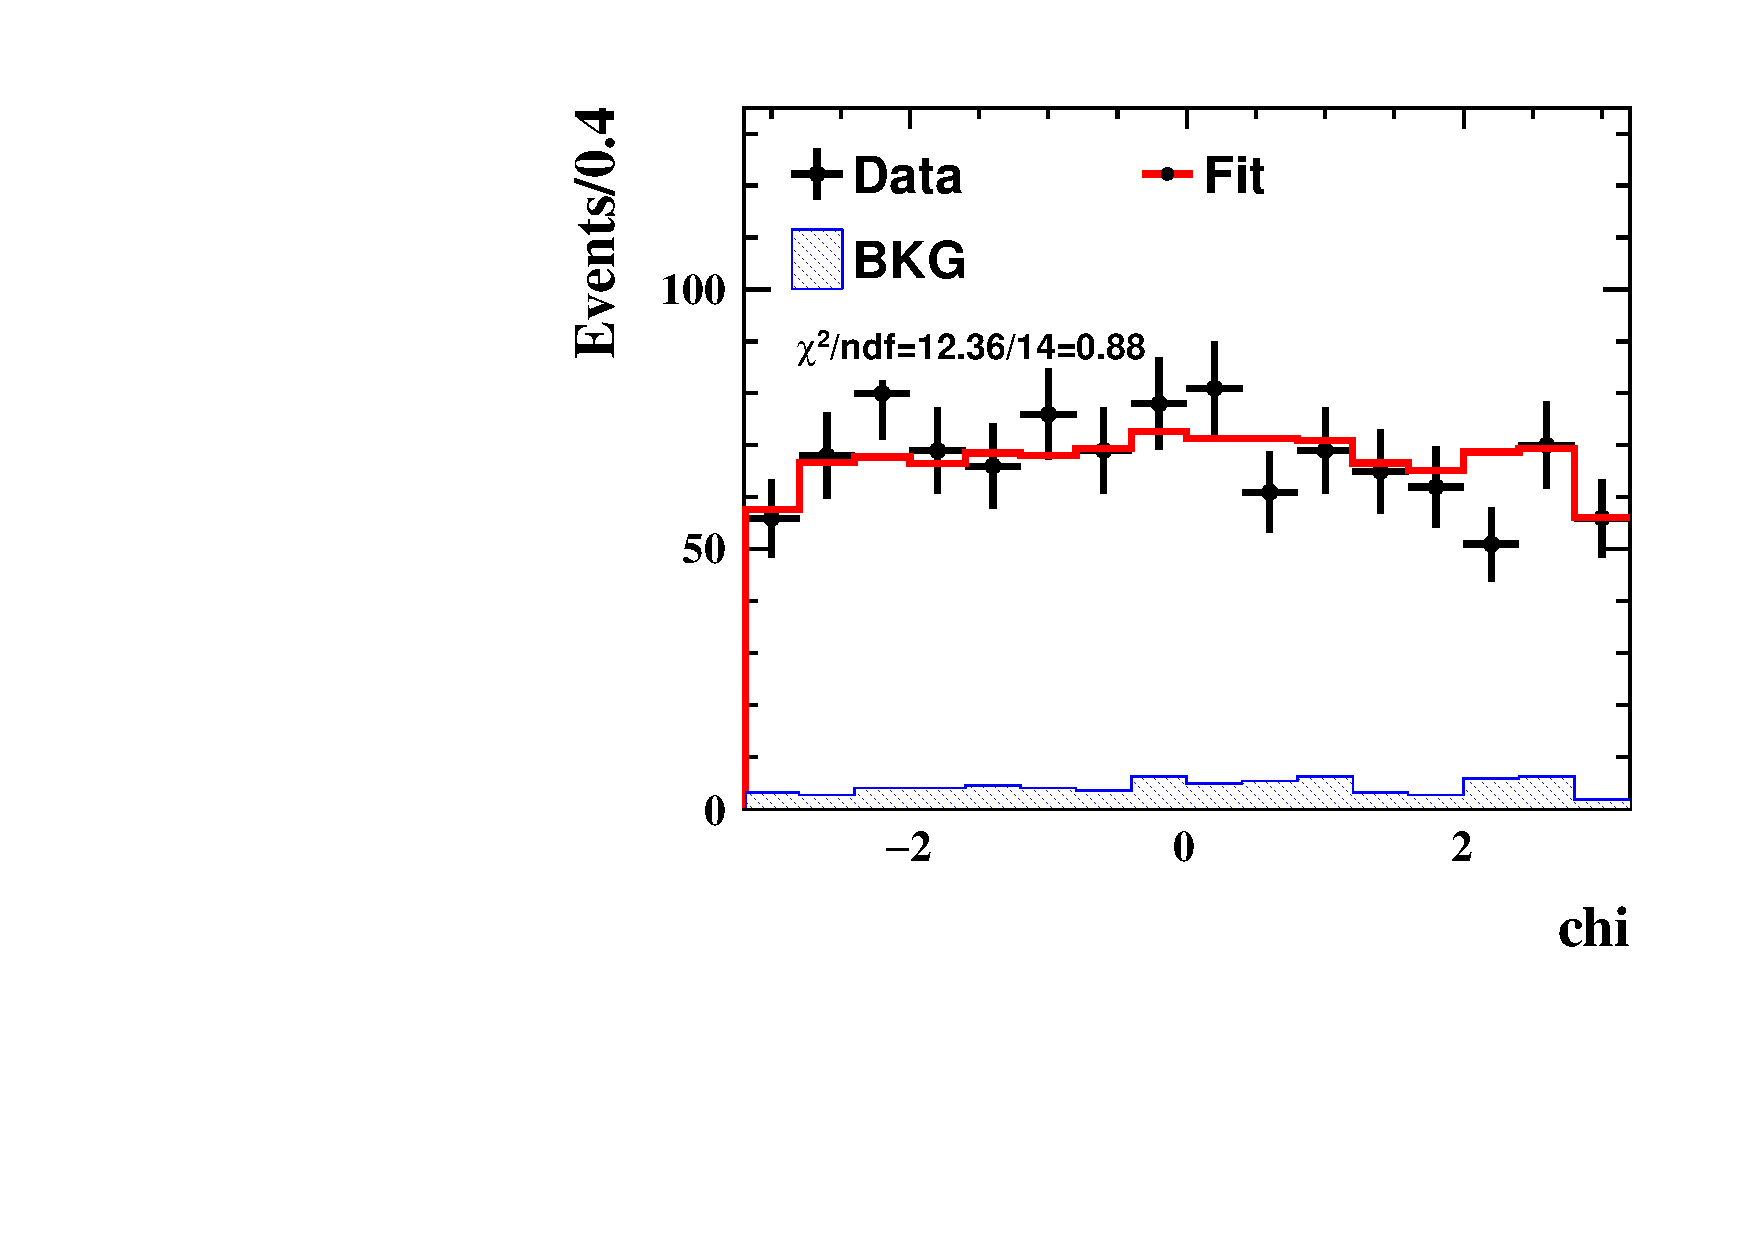
\includegraphics[width=0.24\textwidth]{figure/polarimetery/angular_plots/pkpi_4612_phi2.pdf}
    \caption{Fit results of helicity angles of $\theta_{\lcp}$, $\theta$, $\phi$ and $\chi$ at $\sqrt{s} = 4.612\gev/c^2$.}
\label{fig:fit_angular_s1}
\end{figure}

\begin{figure}[H]\centering
    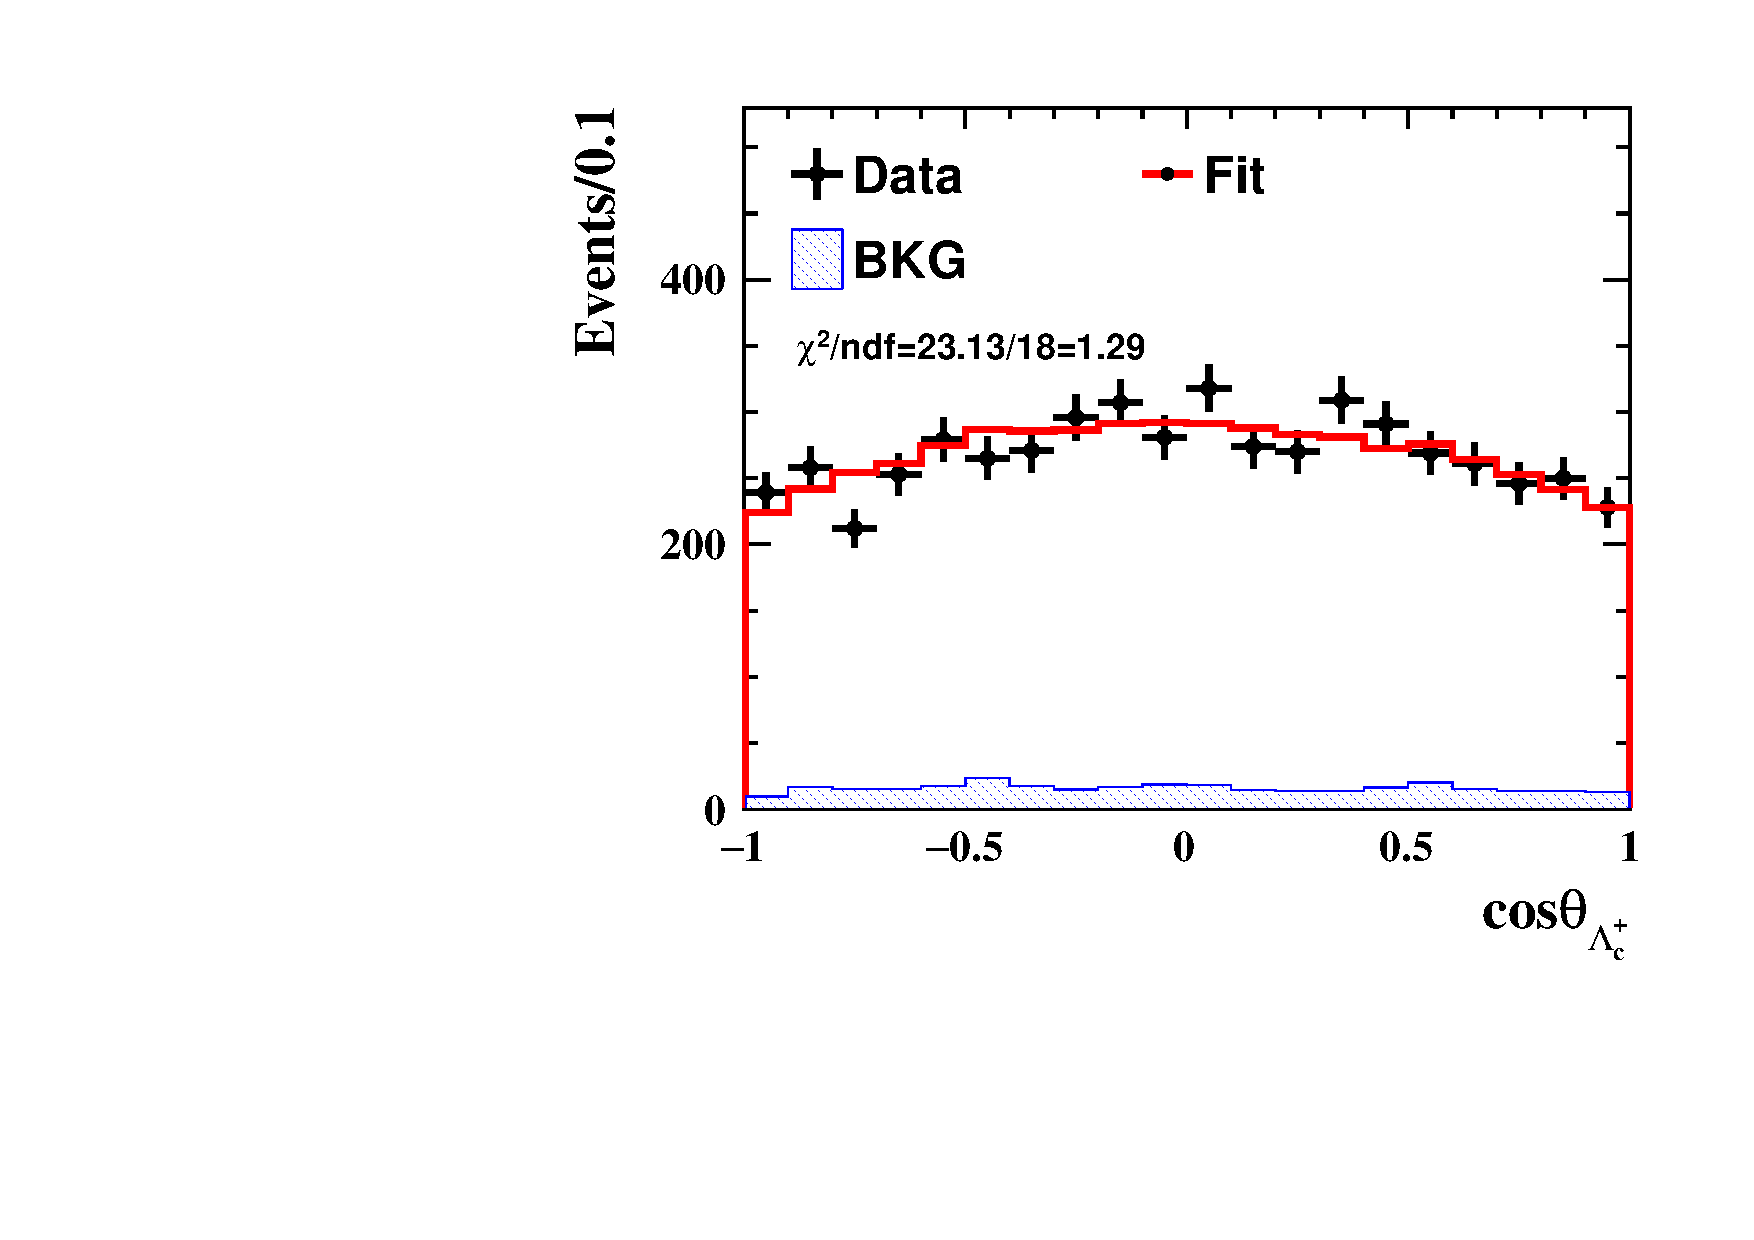
\includegraphics[width=0.24\textwidth]{figure/polarimetery/angular_plots/pkpi_4626_cos_theta0.pdf}
    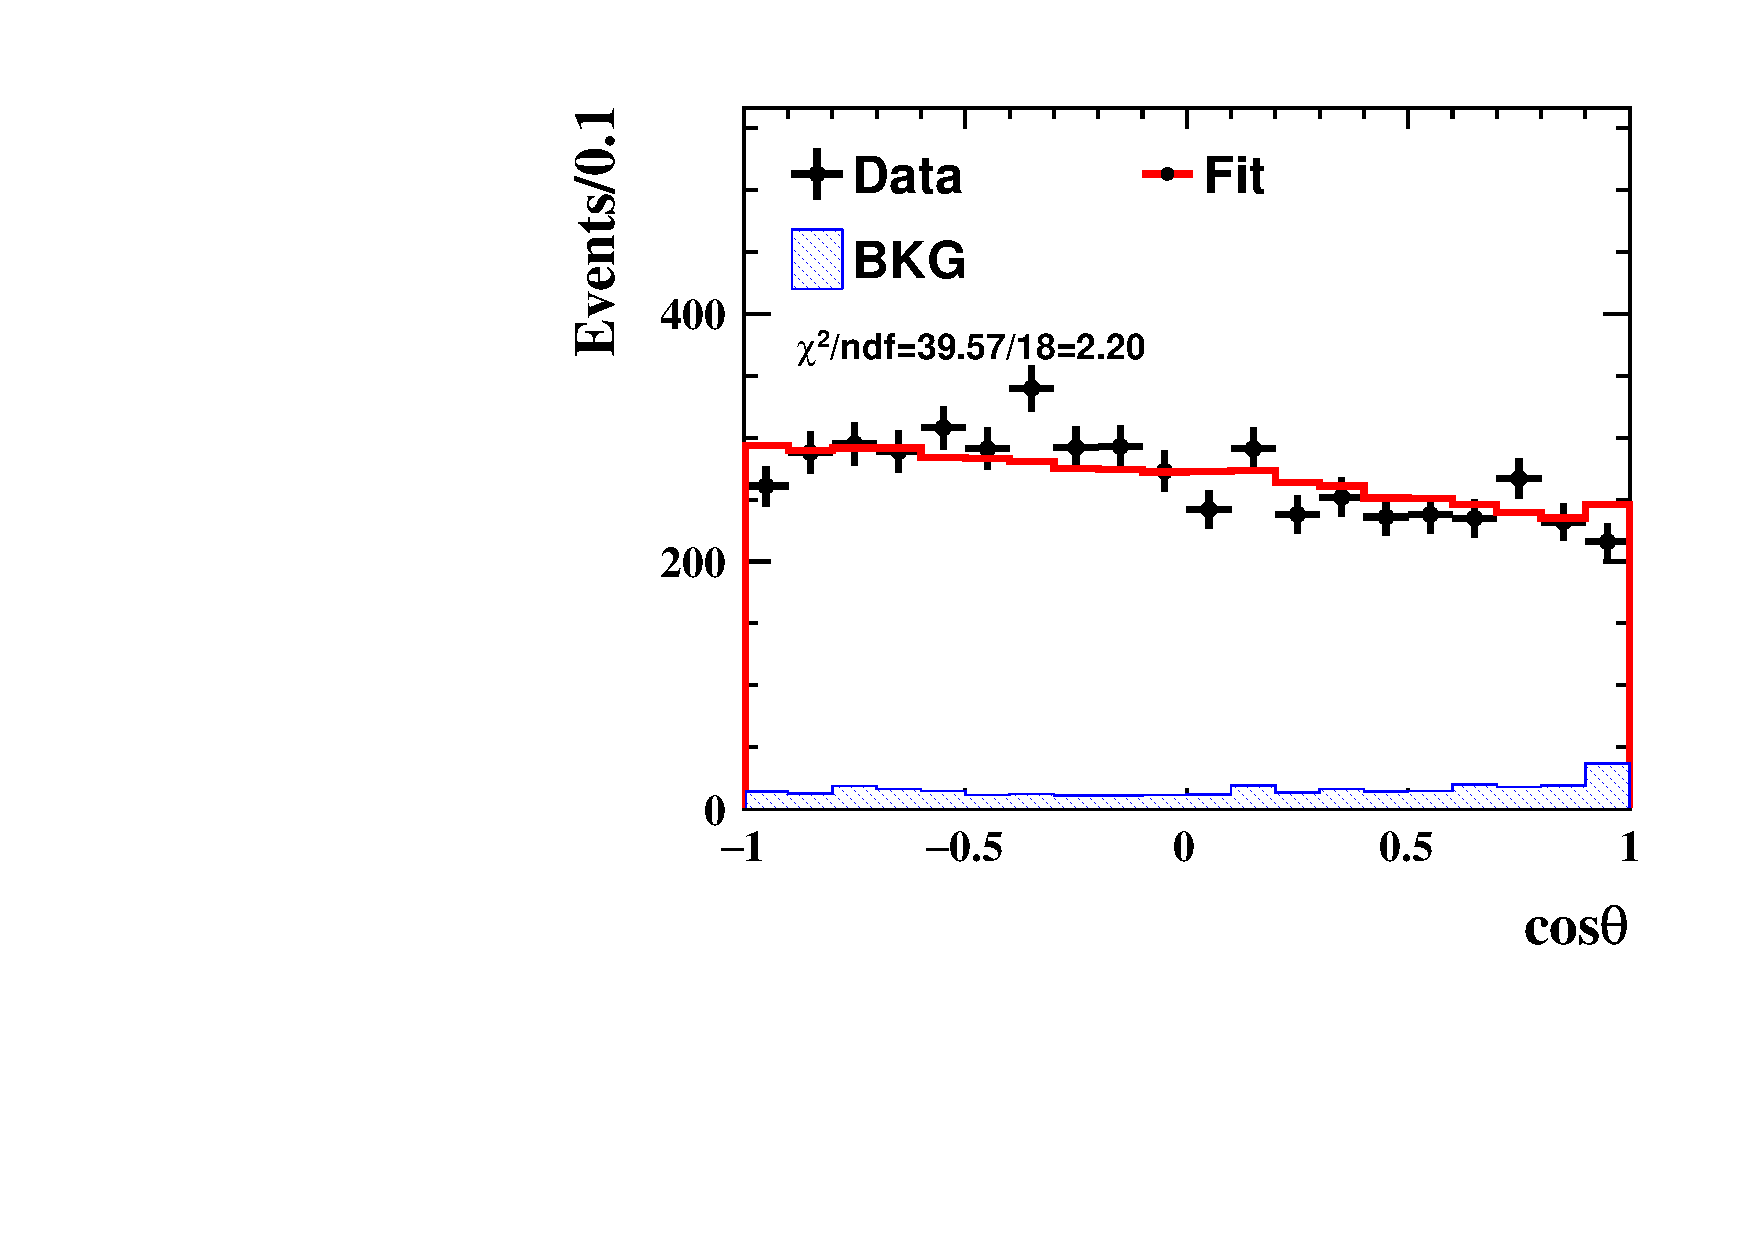
\includegraphics[width=0.24\textwidth]{figure/polarimetery/angular_plots/pkpi_4626_cos_theta1.pdf}
    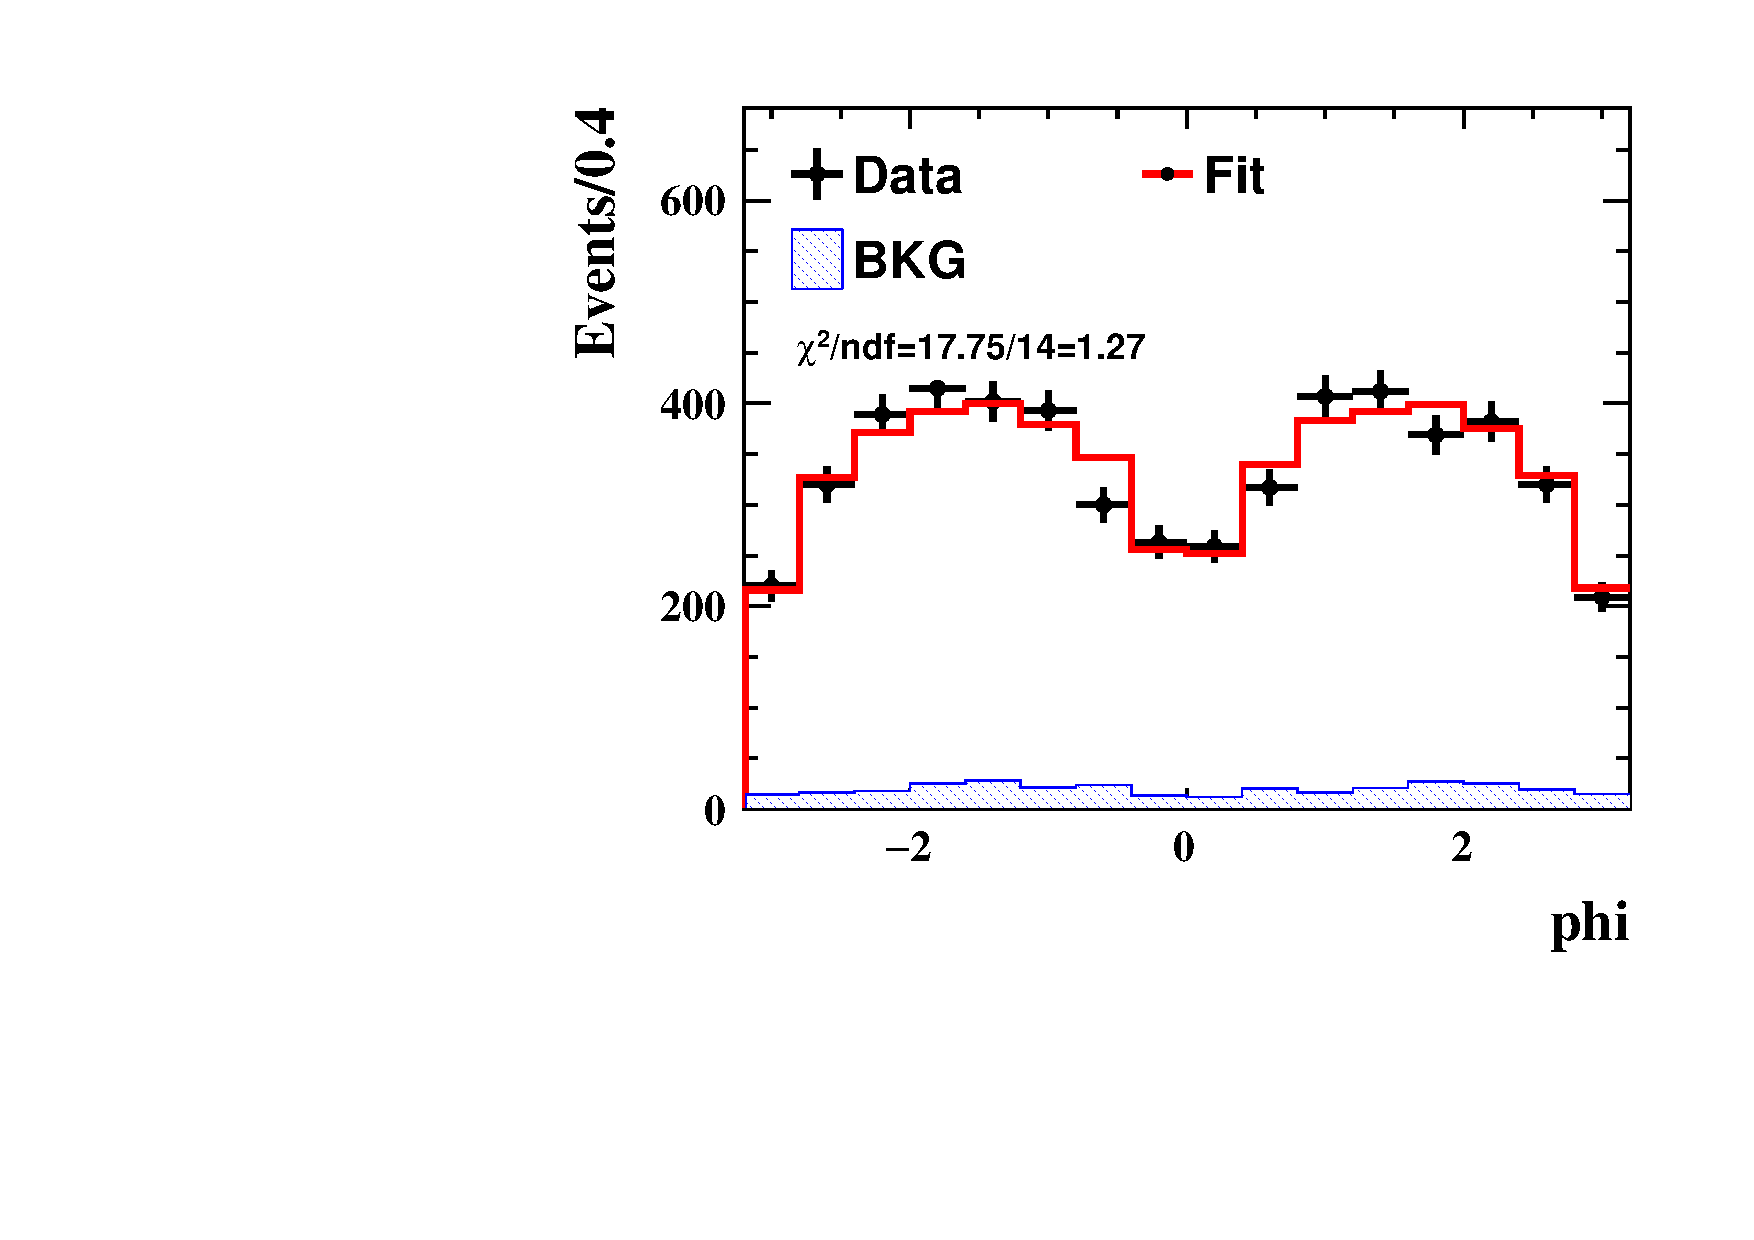
\includegraphics[width=0.24\textwidth]{figure/polarimetery/angular_plots/pkpi_4626_phi1.pdf}
    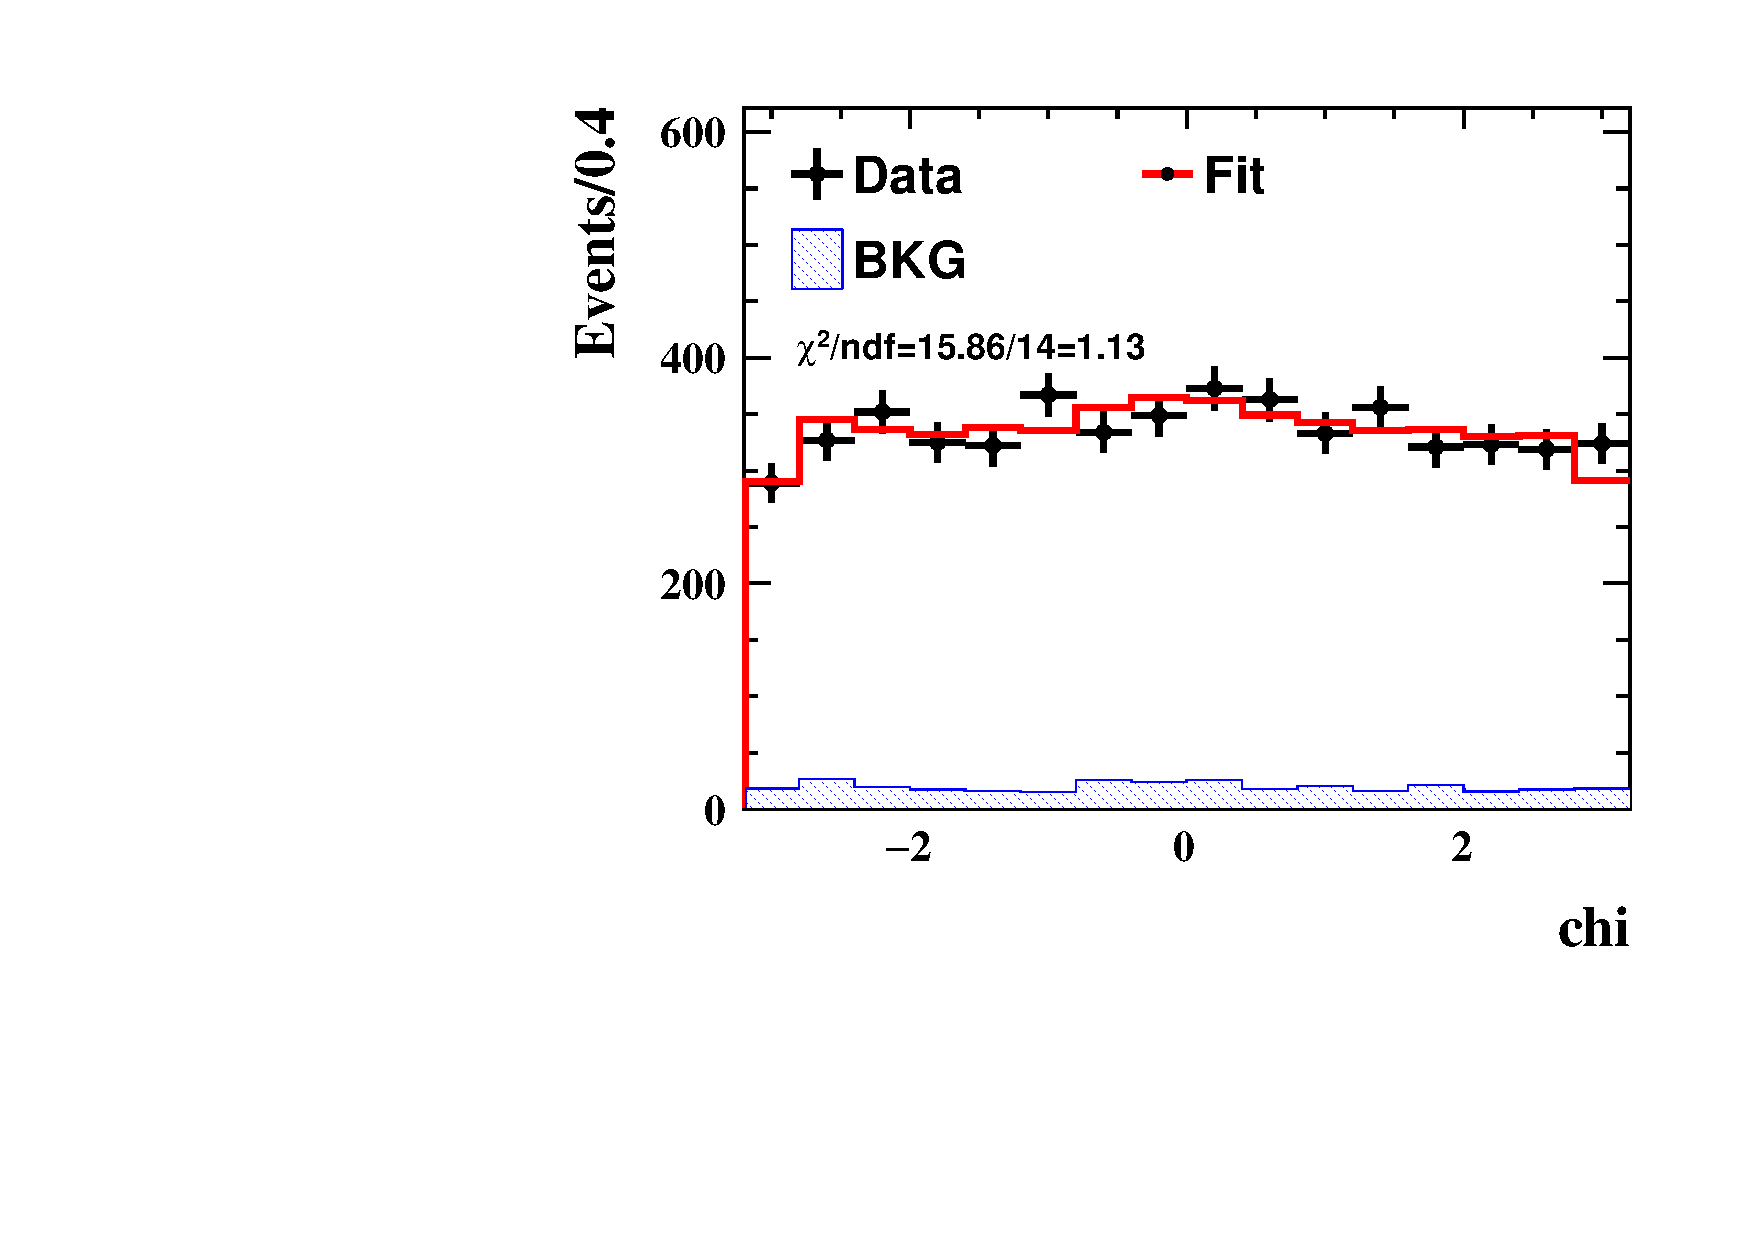
\includegraphics[width=0.24\textwidth]{figure/polarimetery/angular_plots/pkpi_4626_phi2.pdf}
    \caption{Fit results of helicity angles of $\theta_{\lcp}$, $\theta$, $\phi$ and $\chi$ at $\sqrt{s} = 4.628\gev/c^2$.}
\label{fig:fit_angular_s2}
\end{figure}

\begin{figure}[H]\centering
    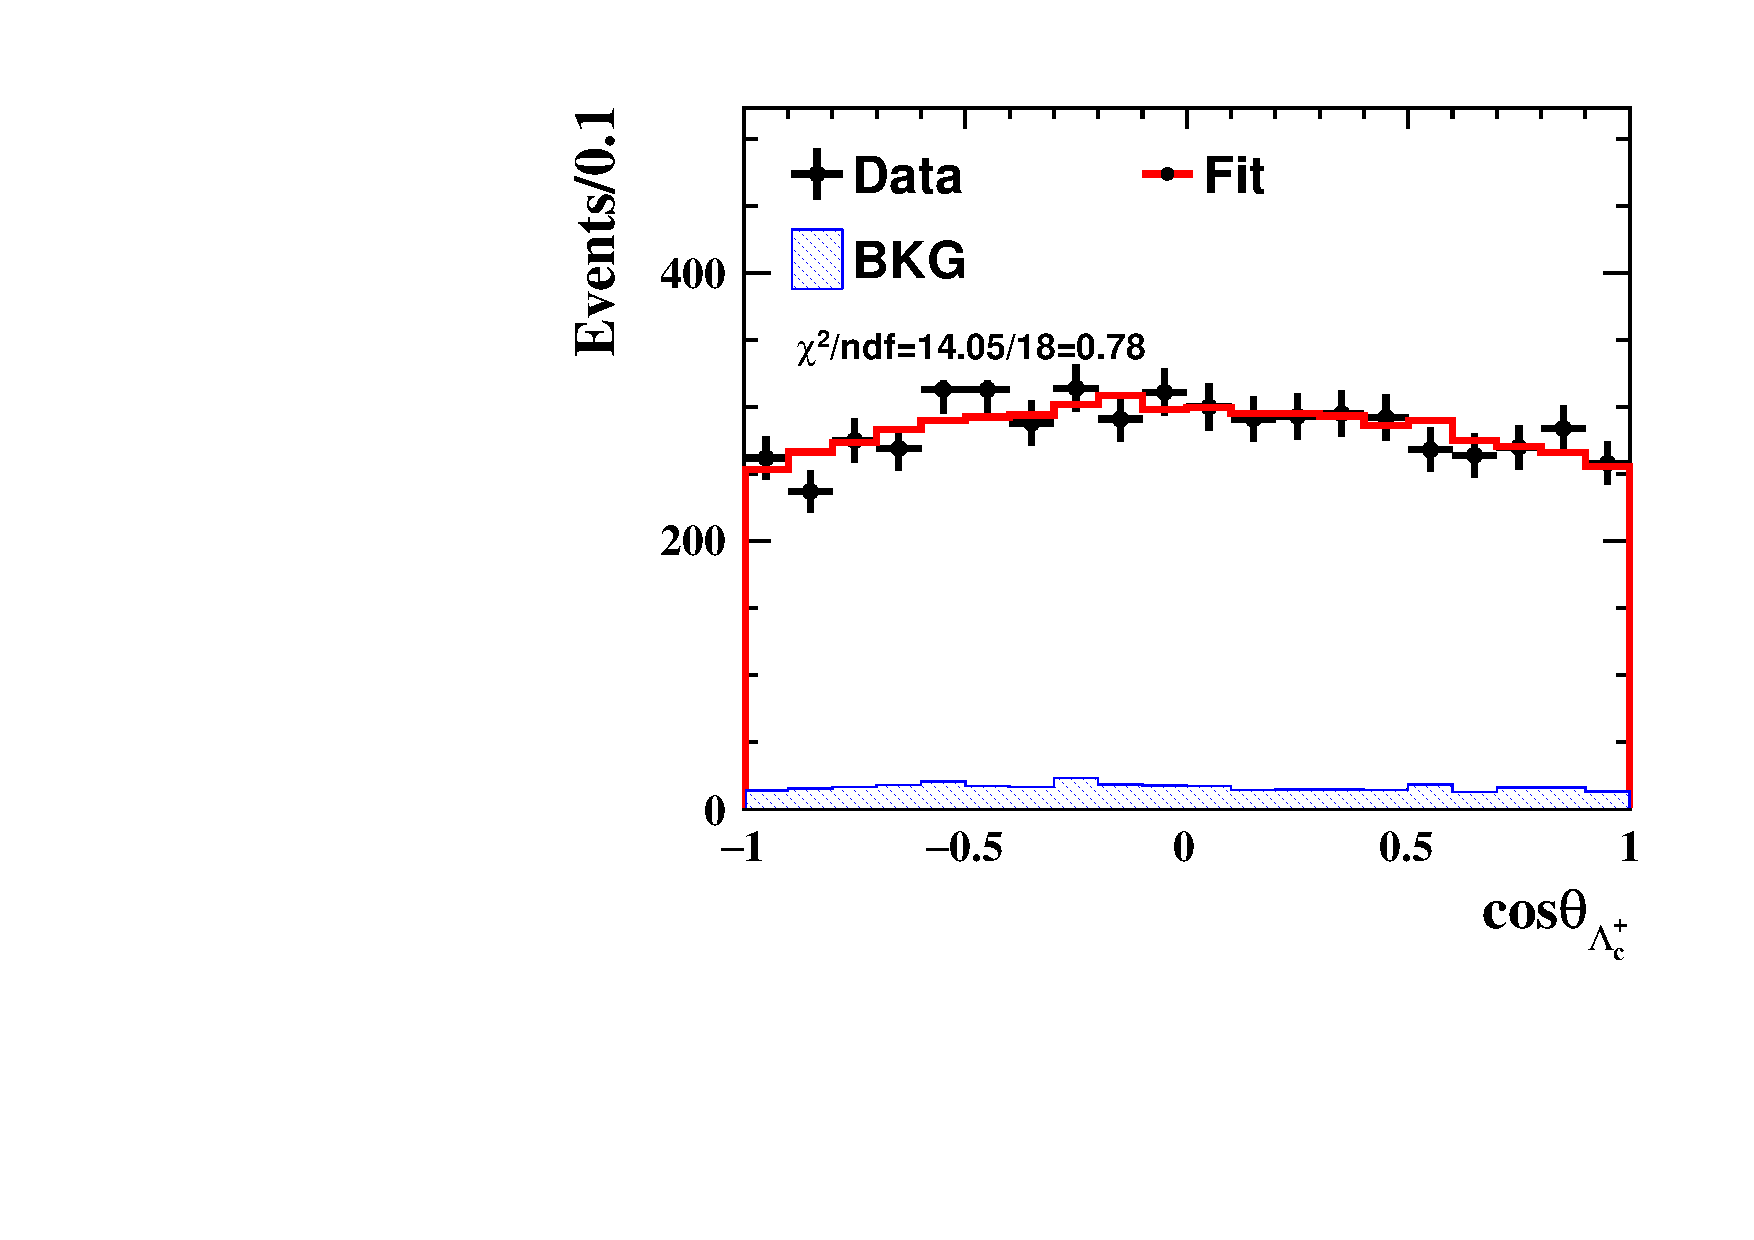
\includegraphics[width=0.24\textwidth]{figure/polarimetery/angular_plots/pkpi_4640_cos_theta0.pdf}
    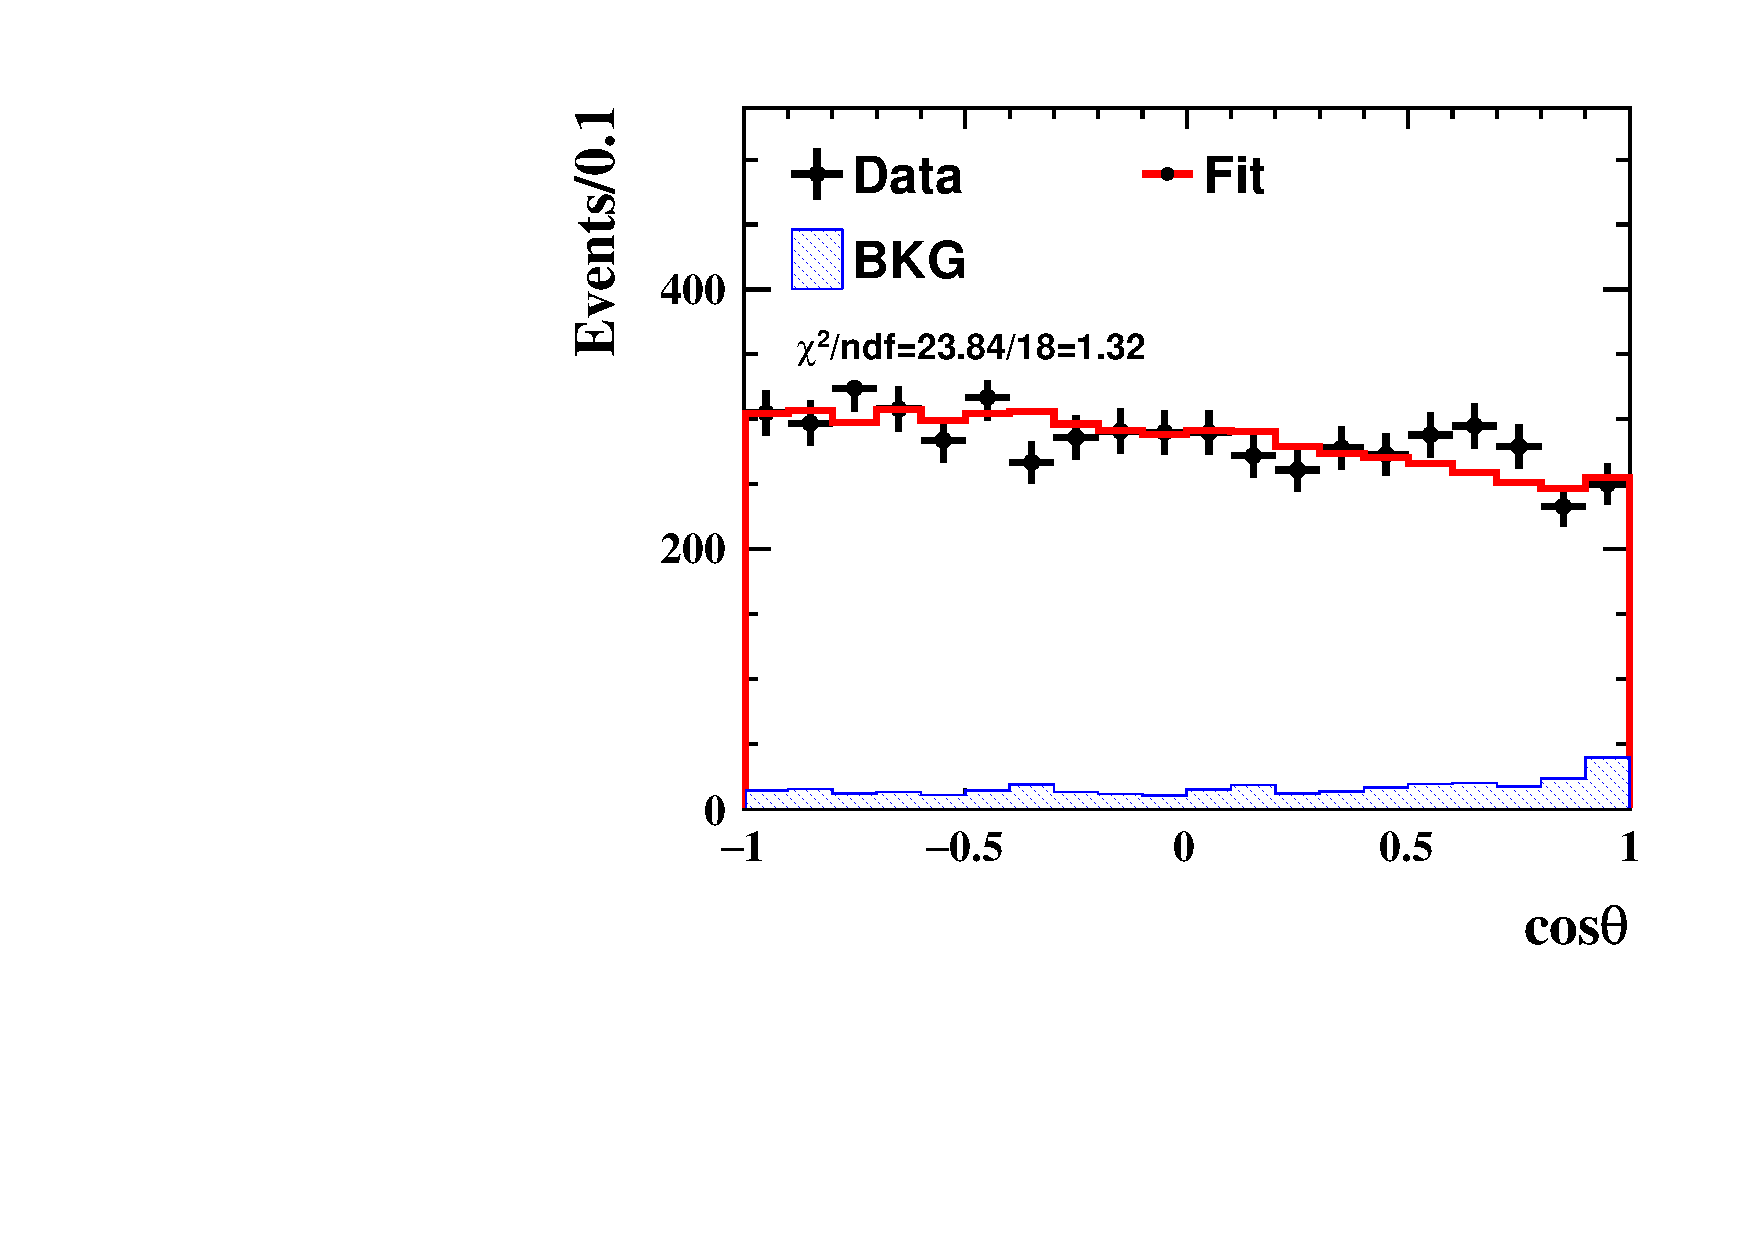
\includegraphics[width=0.24\textwidth]{figure/polarimetery/angular_plots/pkpi_4640_cos_theta1.pdf}
    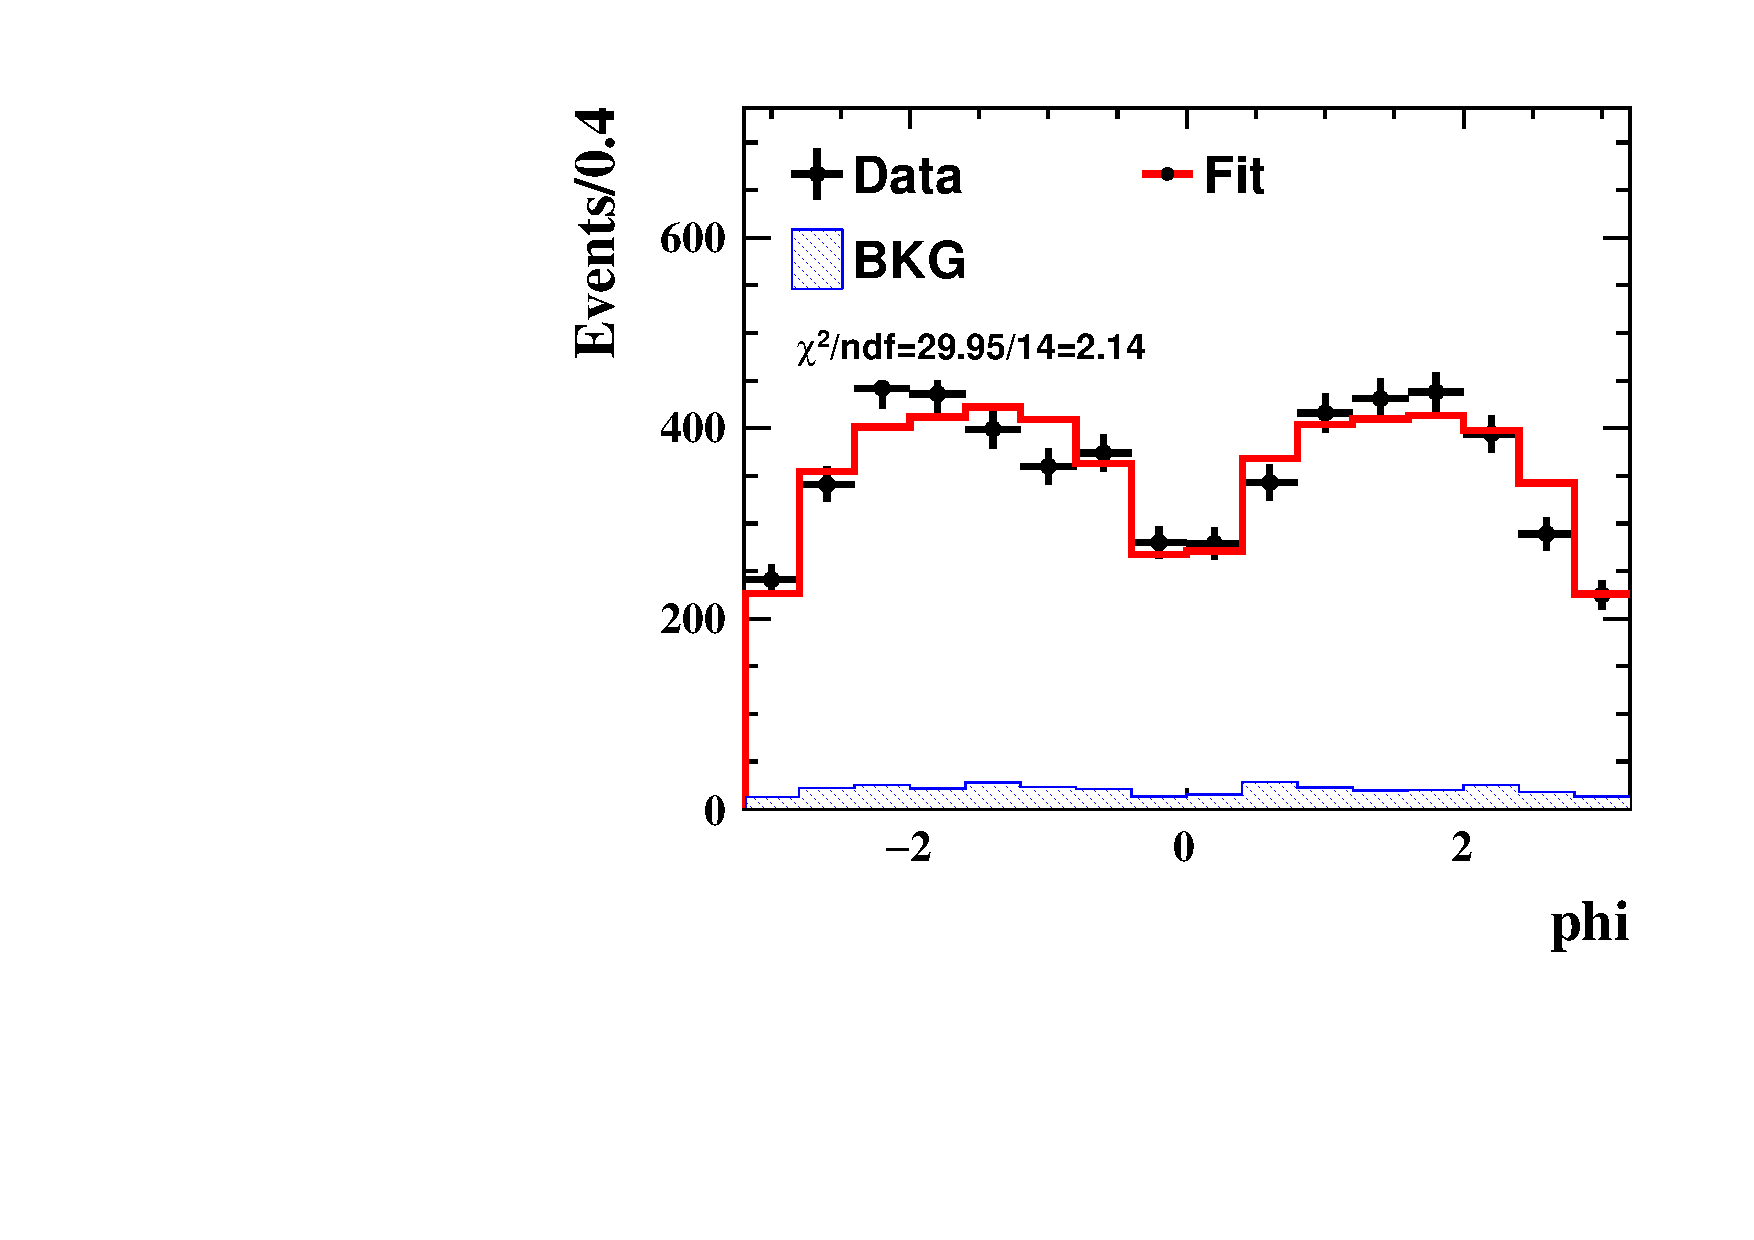
\includegraphics[width=0.24\textwidth]{figure/polarimetery/angular_plots/pkpi_4640_phi1.pdf}
    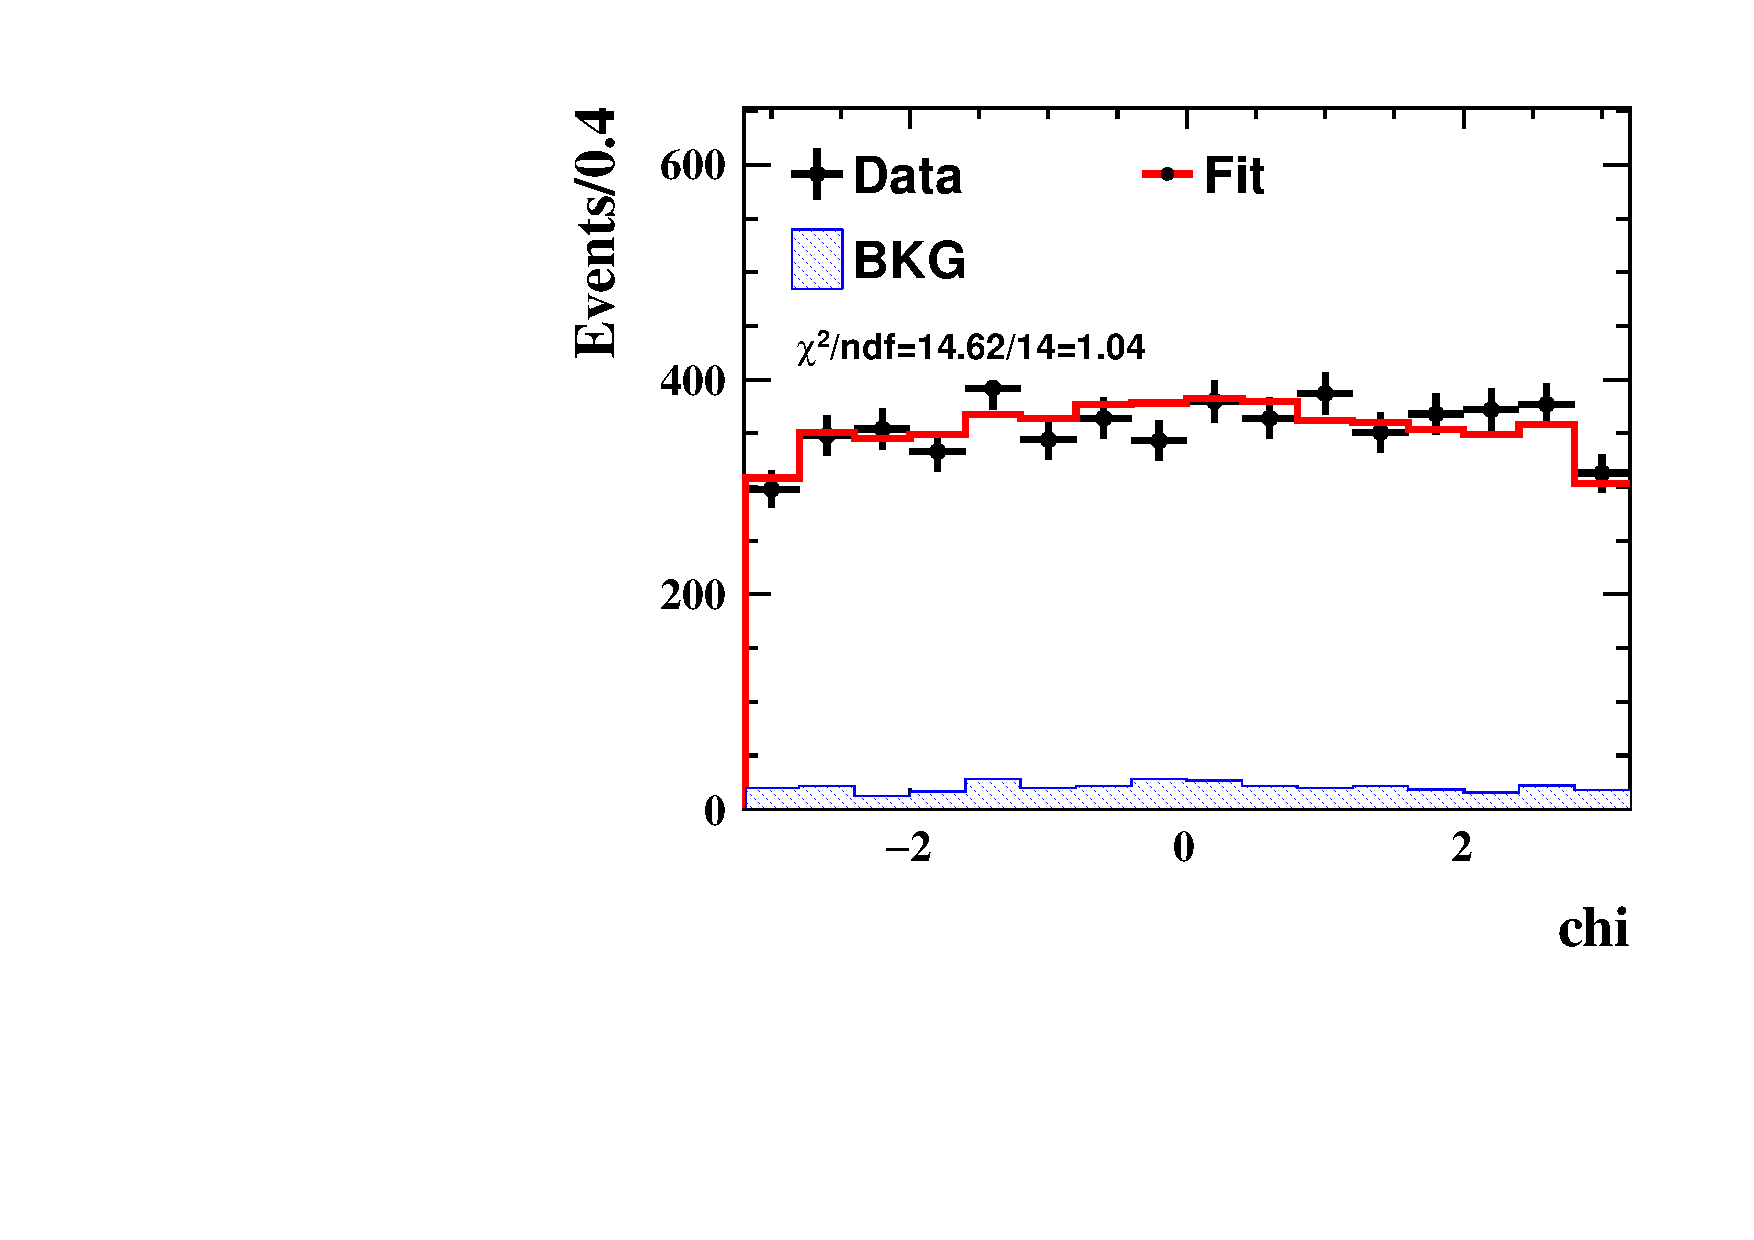
\includegraphics[width=0.24\textwidth]{figure/polarimetery/angular_plots/pkpi_4640_phi2.pdf}
    \caption{Fit results of helicity angles of $\theta_{\lcp}$, $\theta$, $\phi$ and $\chi$ at $\sqrt{s} = 4.641\gev/c^2$.}
\label{fig:fit_angular_s3}
\end{figure}

\begin{figure}[H]\centering
    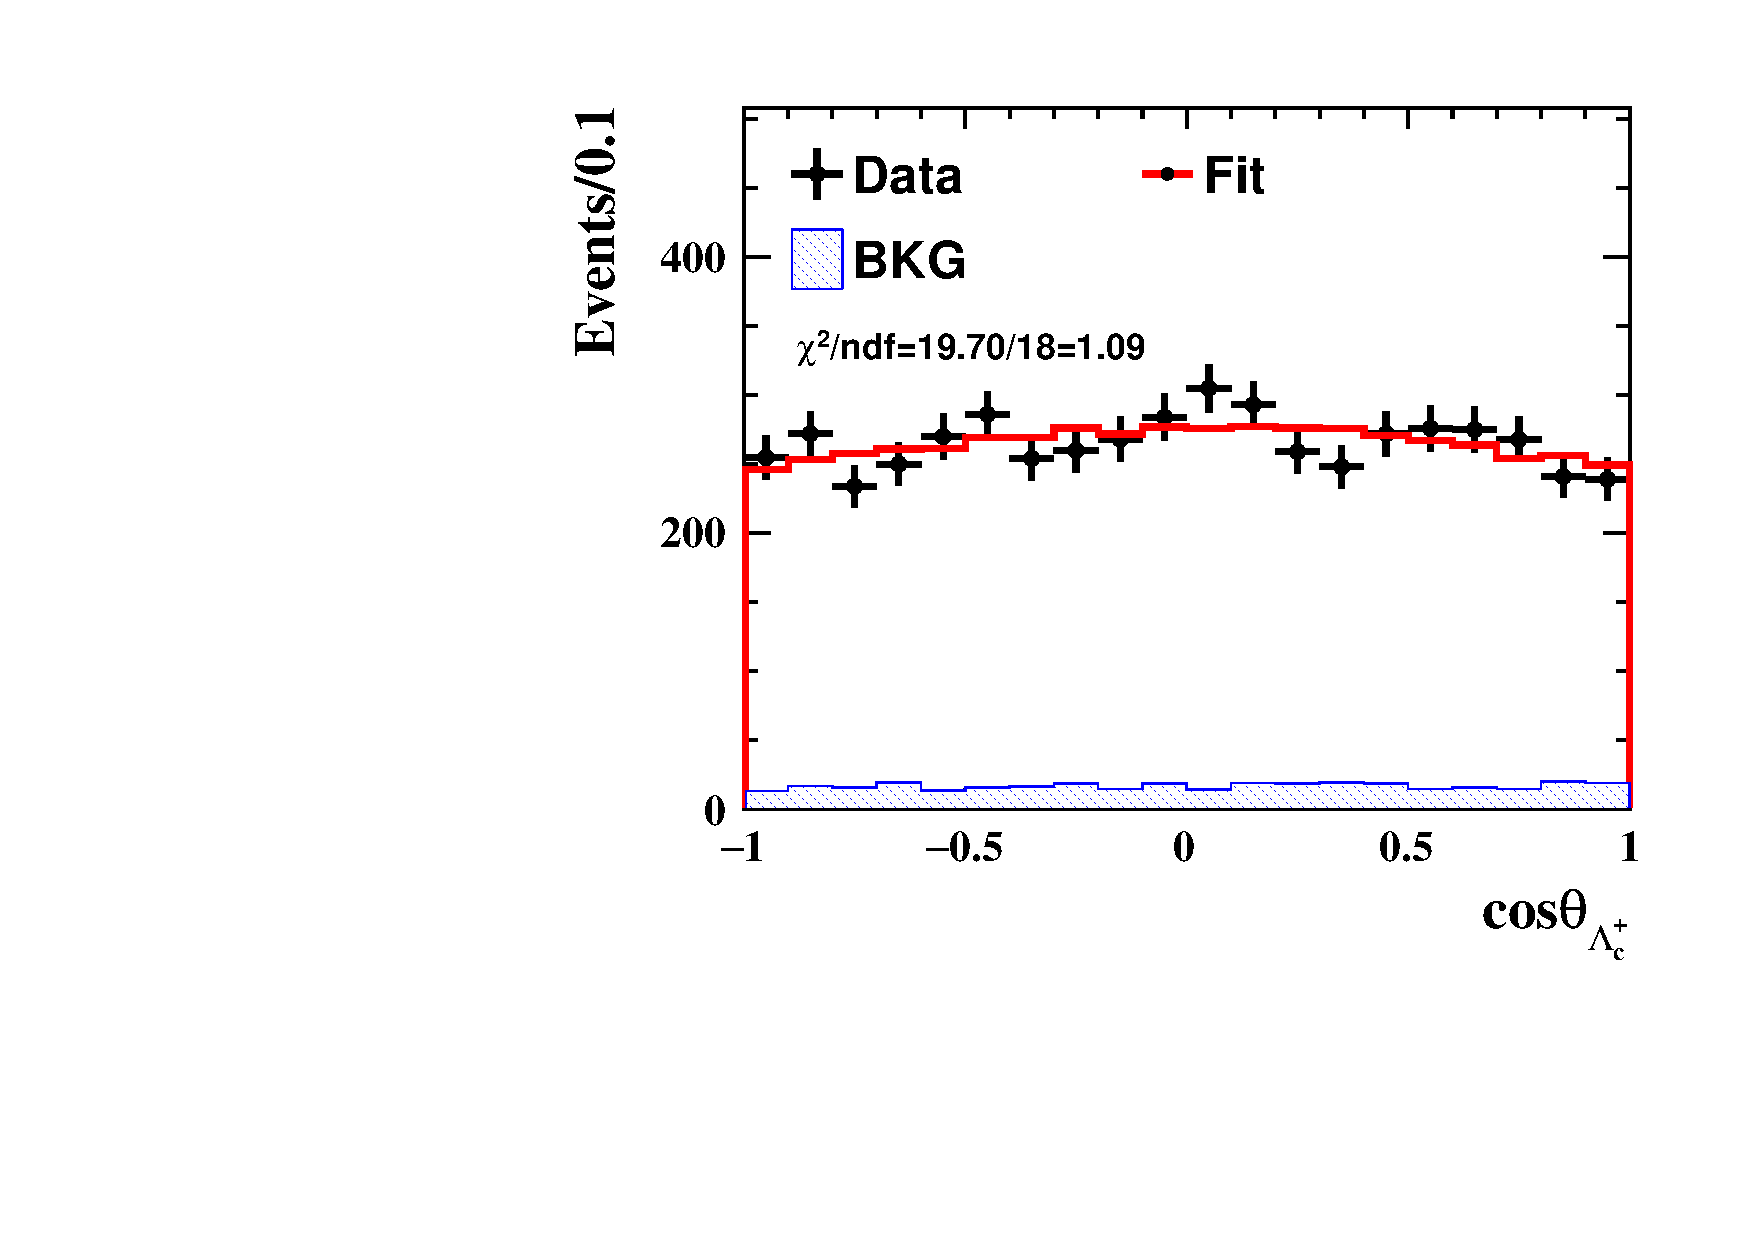
\includegraphics[width=0.24\textwidth]{figure/polarimetery/angular_plots/pkpi_4660_cos_theta0.pdf}
    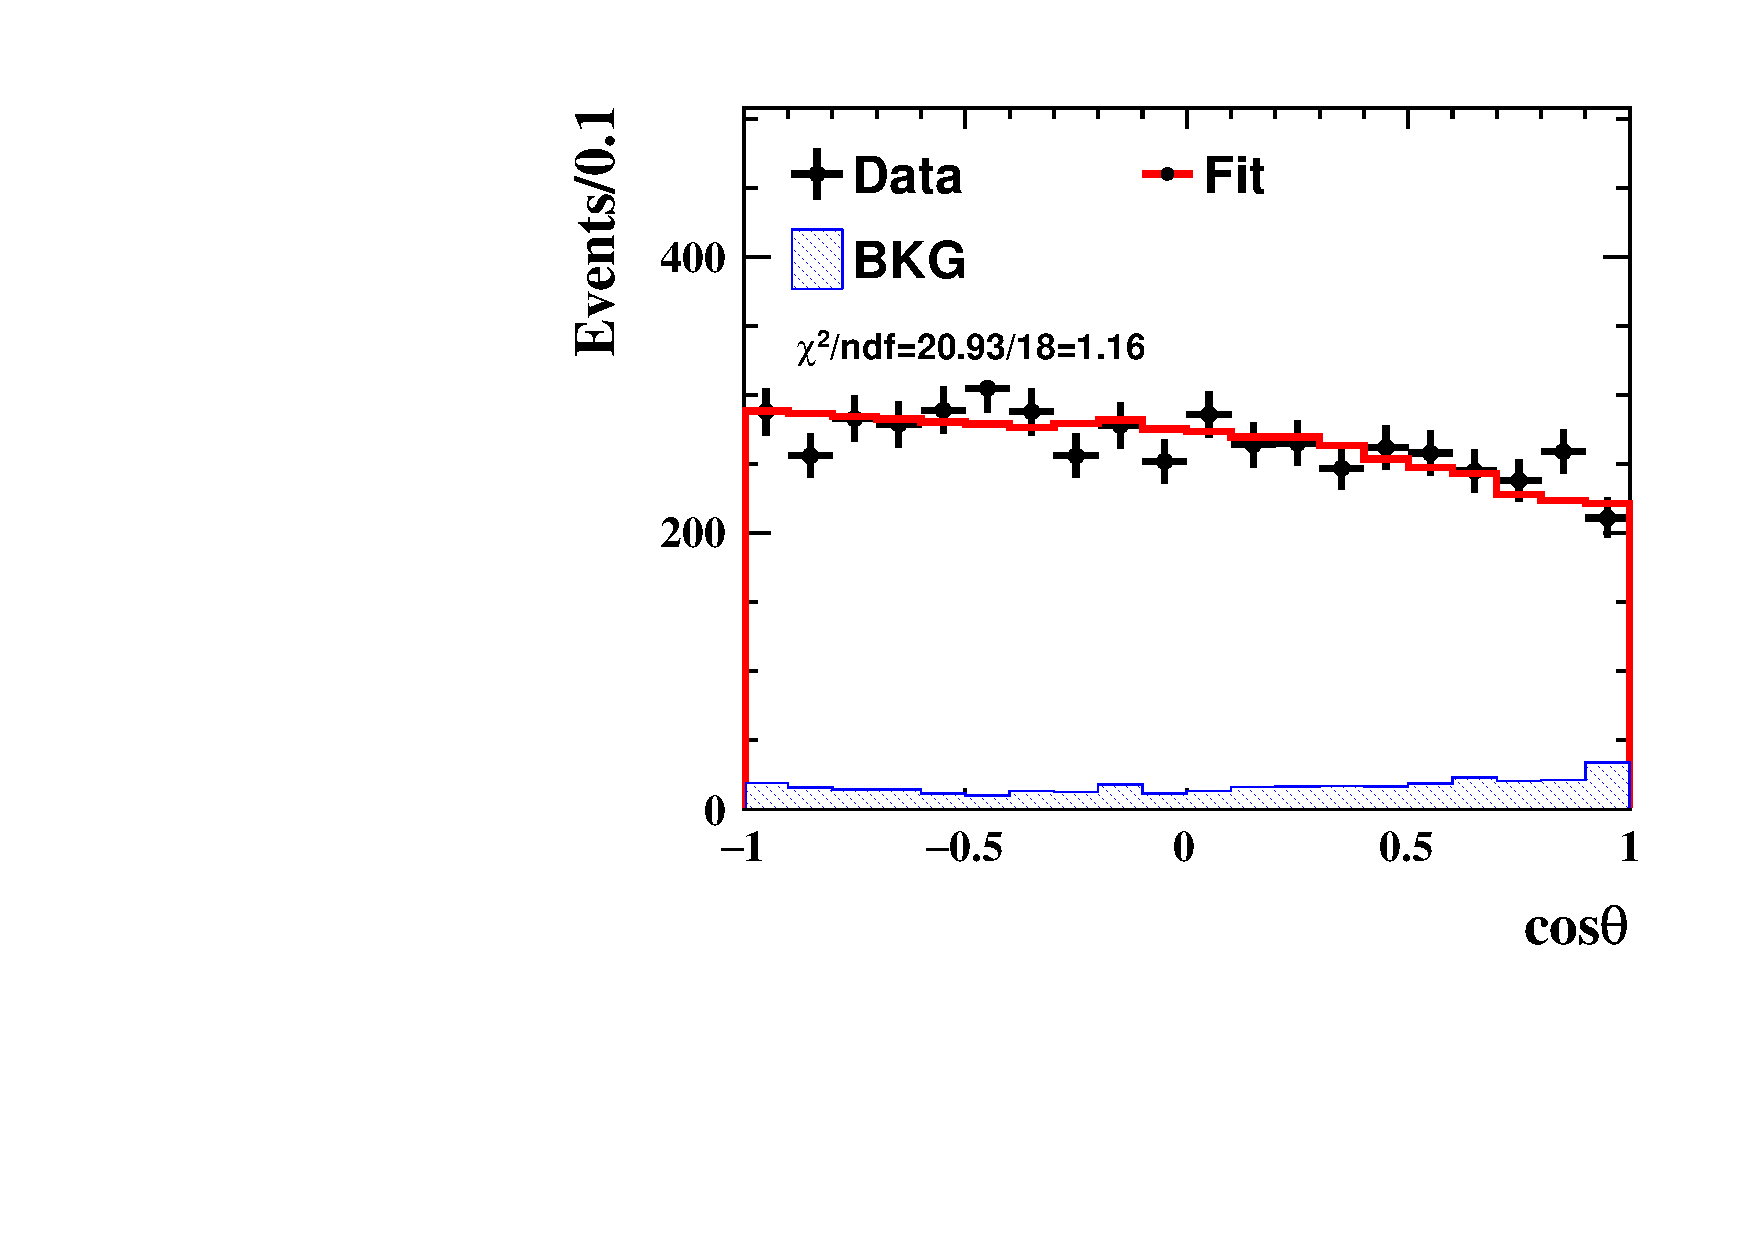
\includegraphics[width=0.24\textwidth]{figure/polarimetery/angular_plots/pkpi_4660_cos_theta1.pdf}
    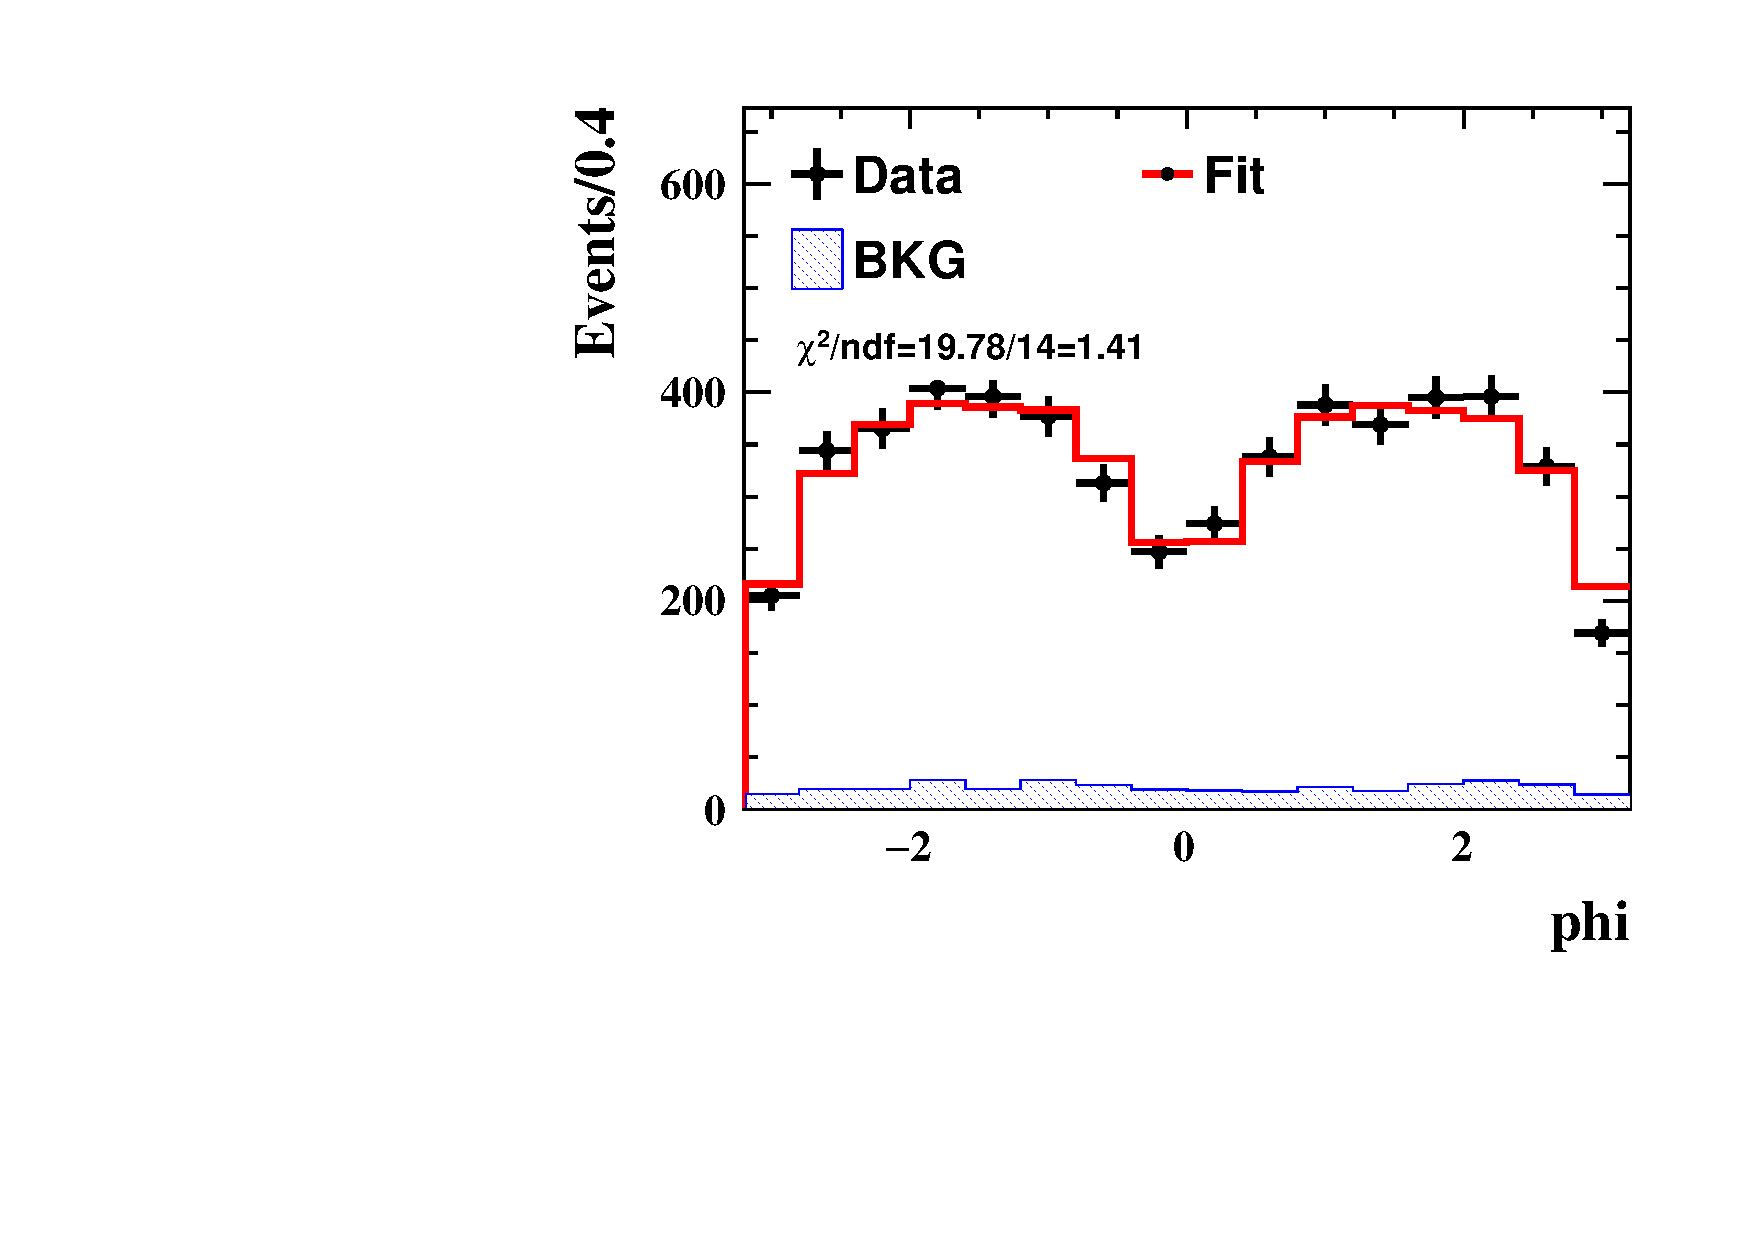
\includegraphics[width=0.24\textwidth]{figure/polarimetery/angular_plots/pkpi_4660_phi1.pdf}
    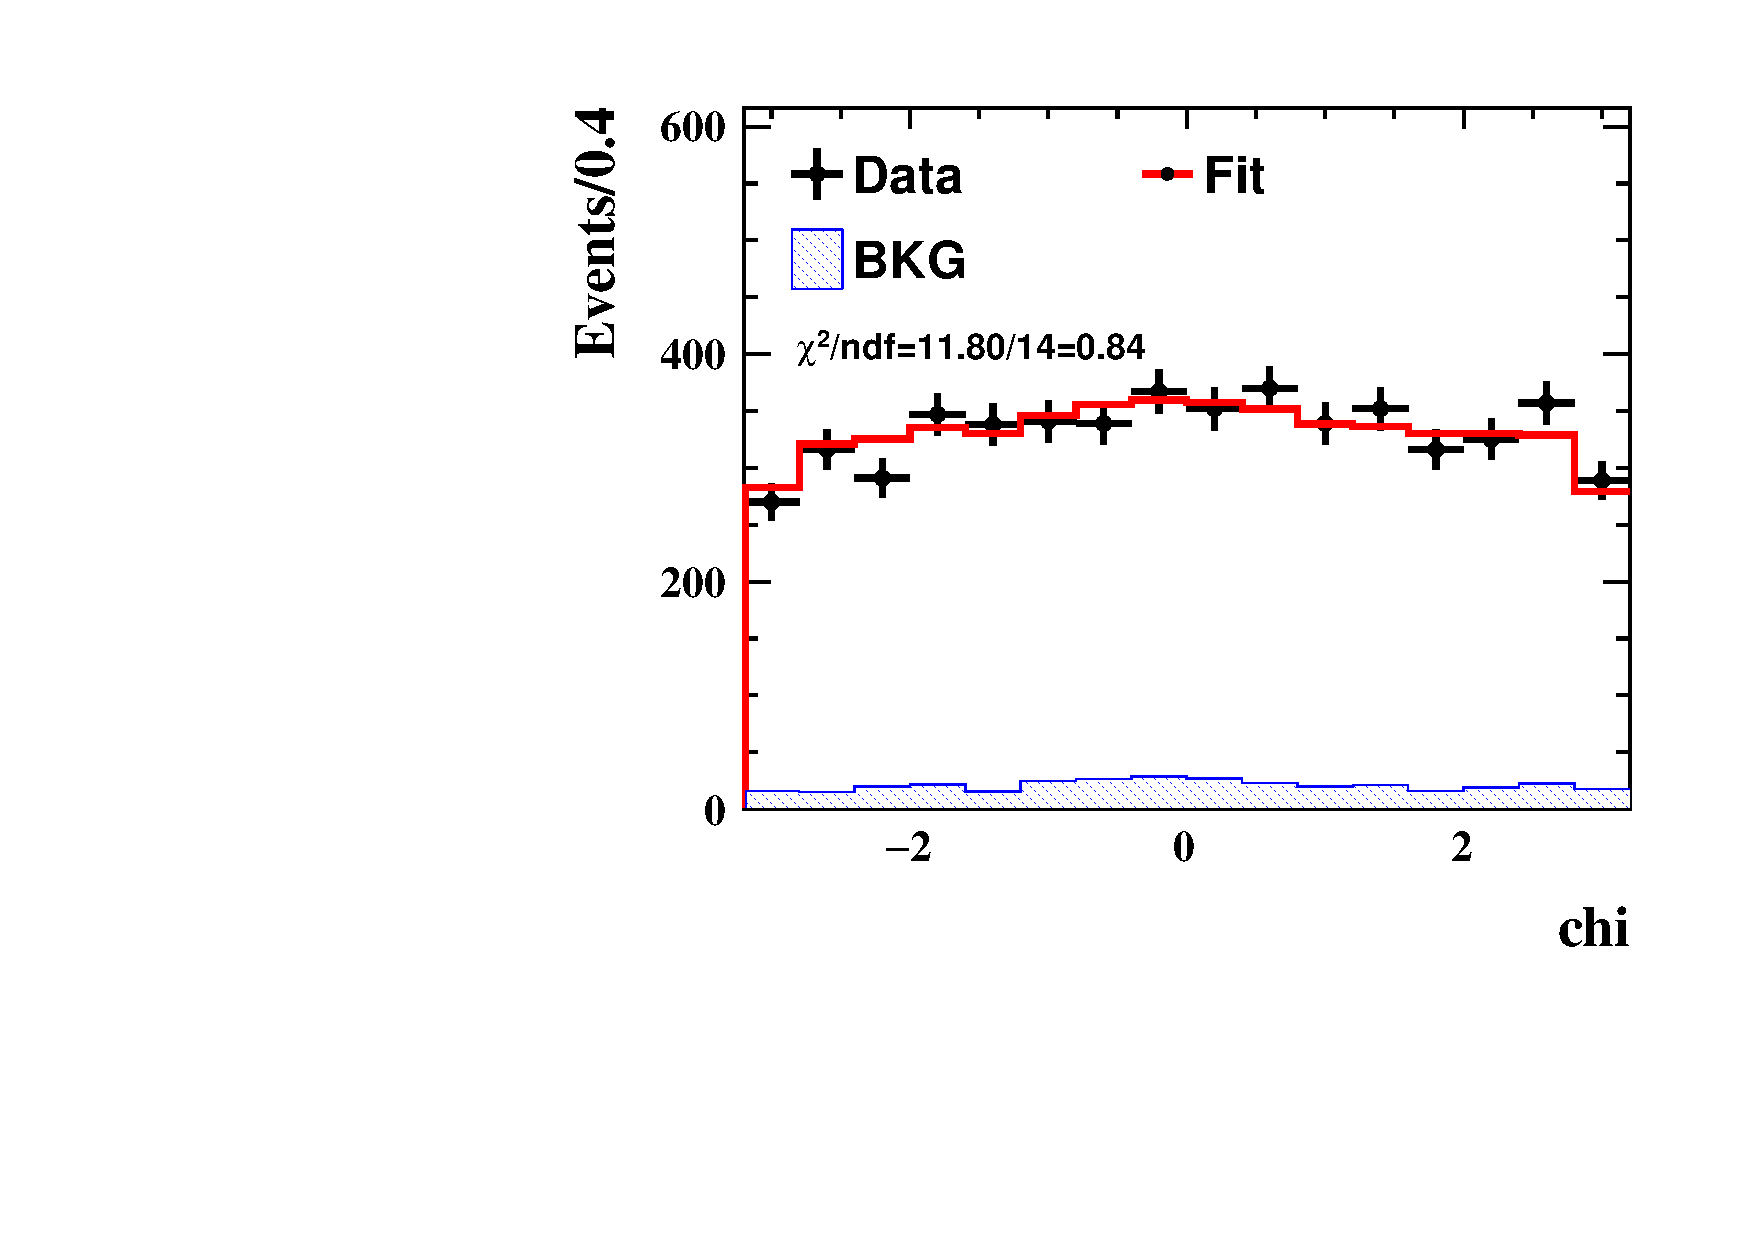
\includegraphics[width=0.24\textwidth]{figure/polarimetery/angular_plots/pkpi_4660_phi2.pdf}
    \caption{Fit results of helicity angles of $\theta_{\lcp}$, $\theta$, $\phi$ and $\chi$ at $\sqrt{s} = 4.661\gev/c^2$.}
\label{fig:fit_angular_s4}
\end{figure}

\begin{figure}[H]\centering
    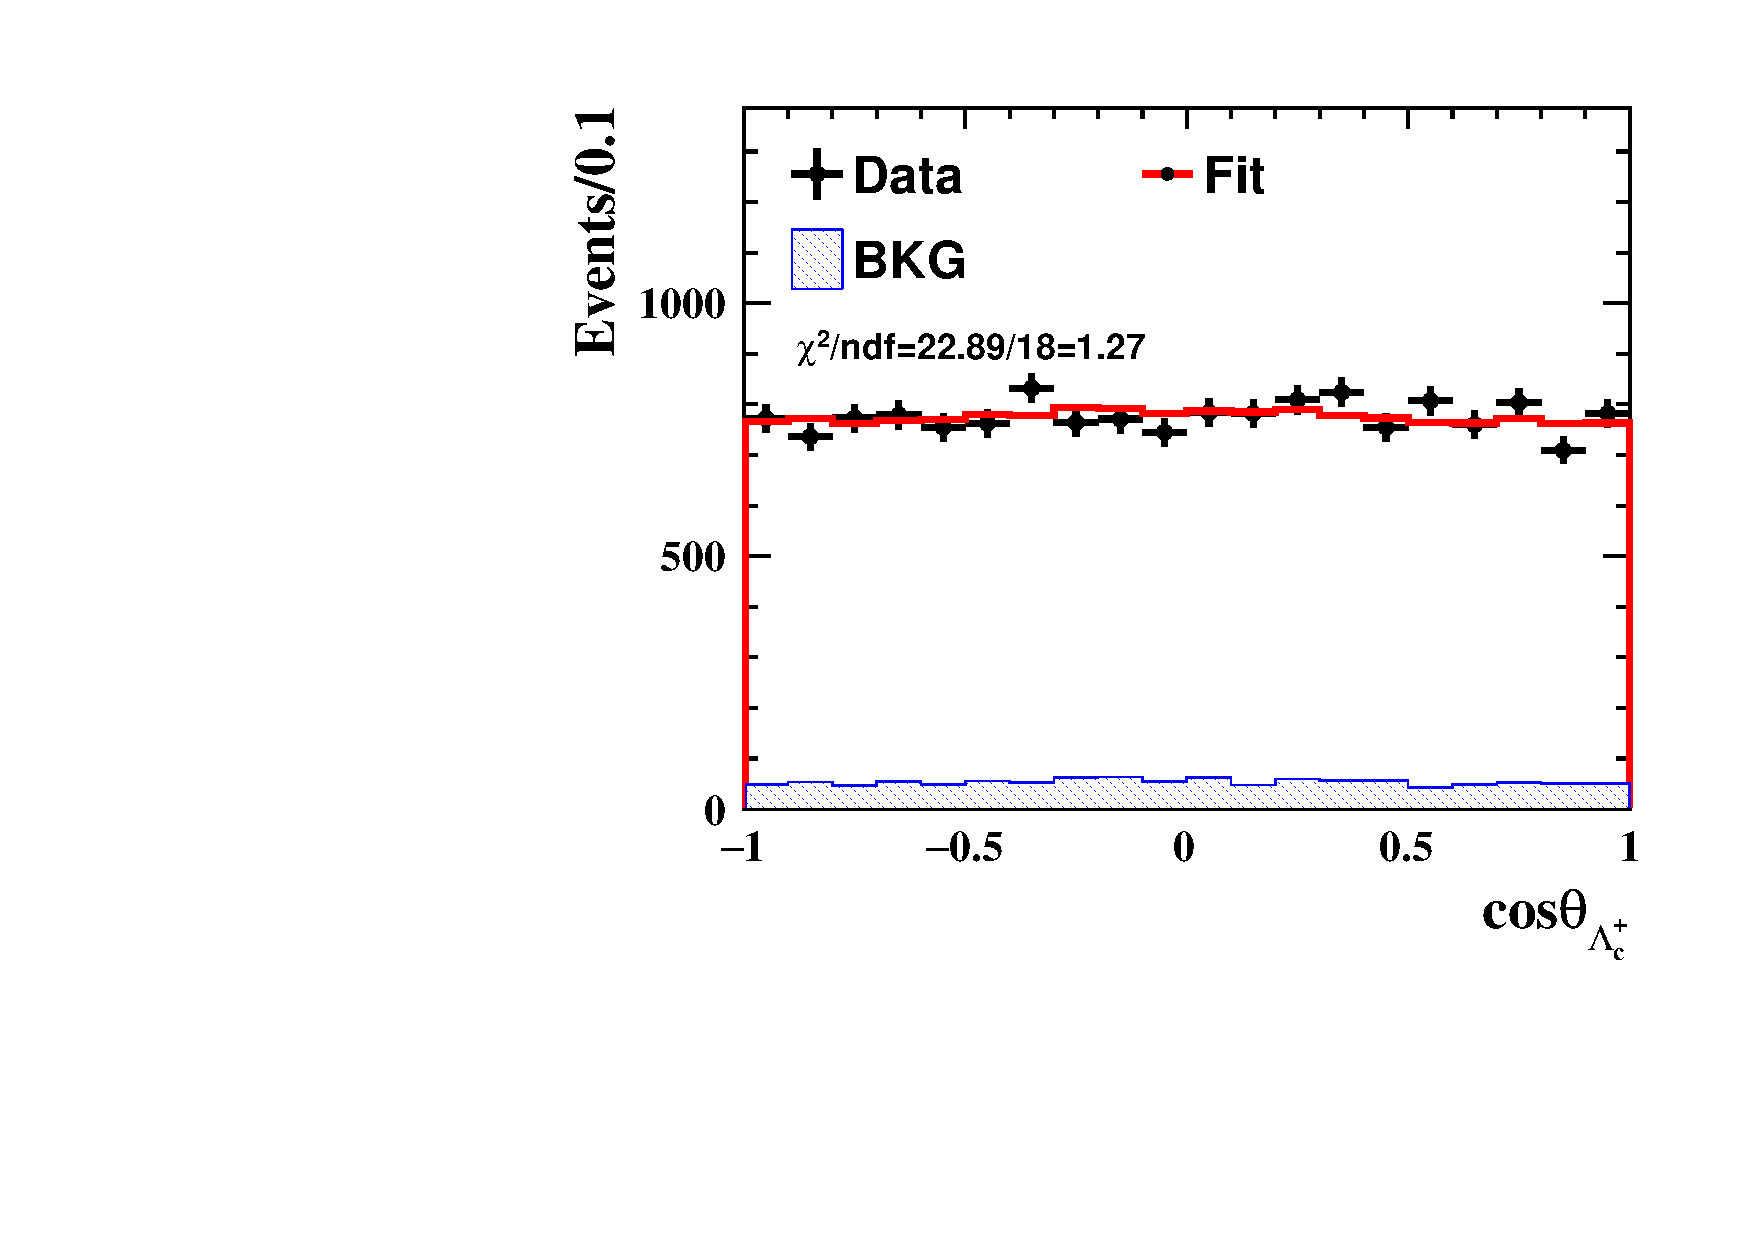
\includegraphics[width=0.24\textwidth]{figure/polarimetery/angular_plots/pkpi_4680_cos_theta0.pdf}
    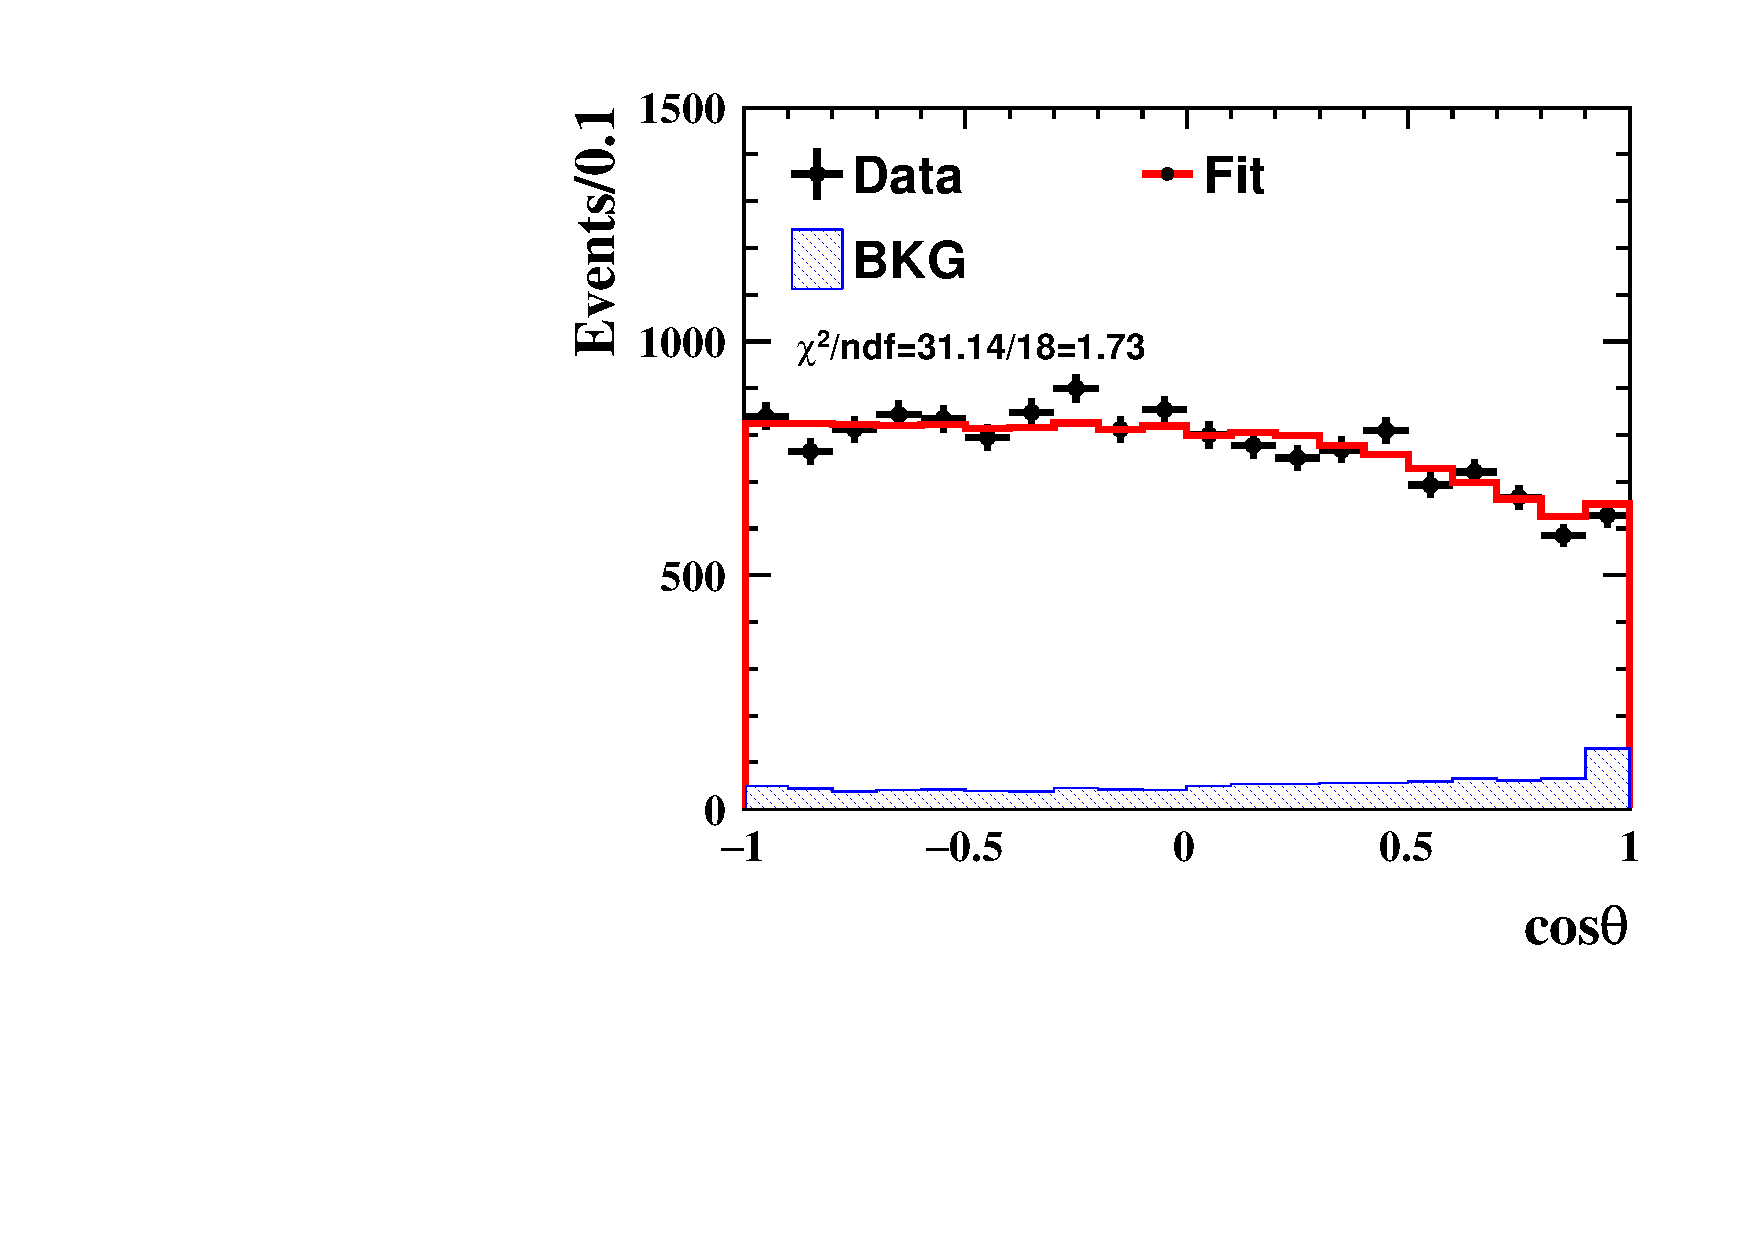
\includegraphics[width=0.24\textwidth]{figure/polarimetery/angular_plots/pkpi_4680_cos_theta1.pdf}
    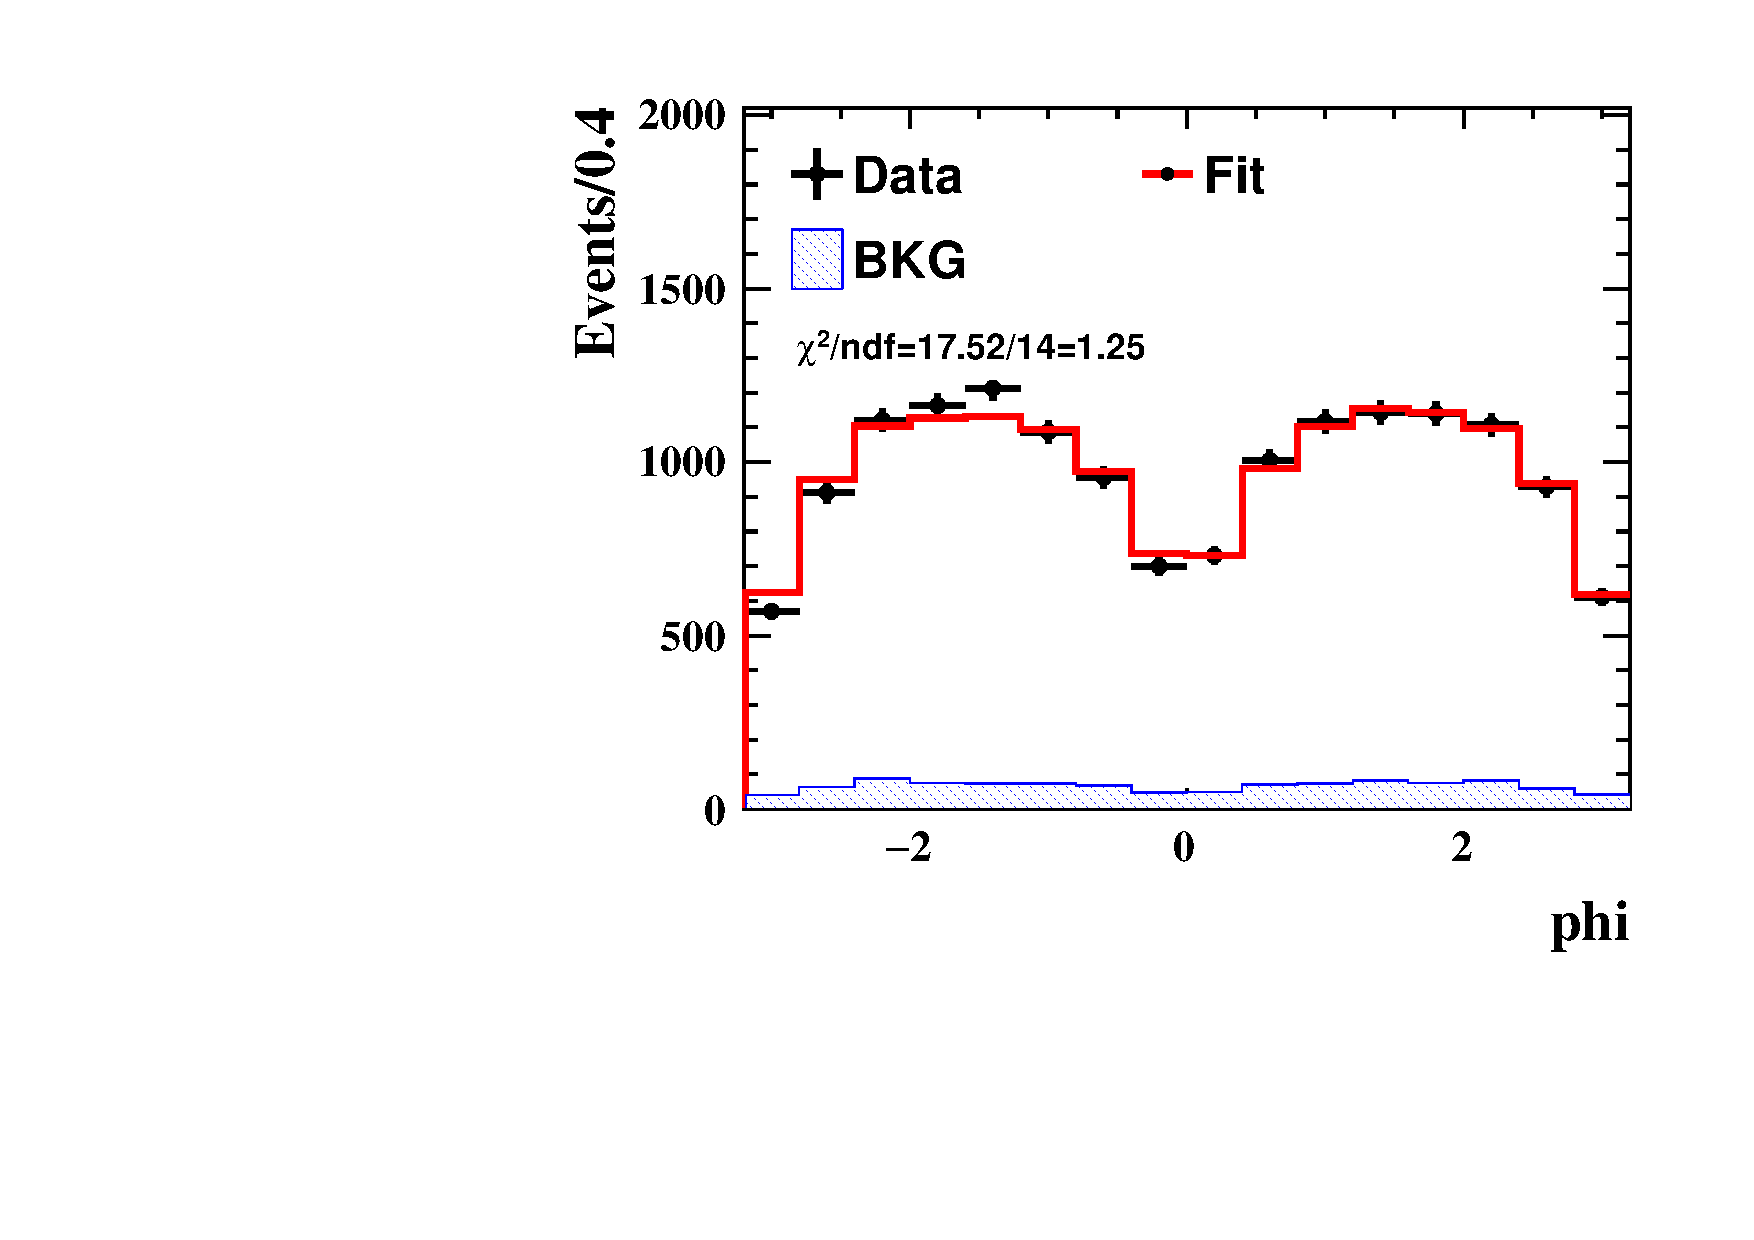
\includegraphics[width=0.24\textwidth]{figure/polarimetery/angular_plots/pkpi_4680_phi1.pdf}
    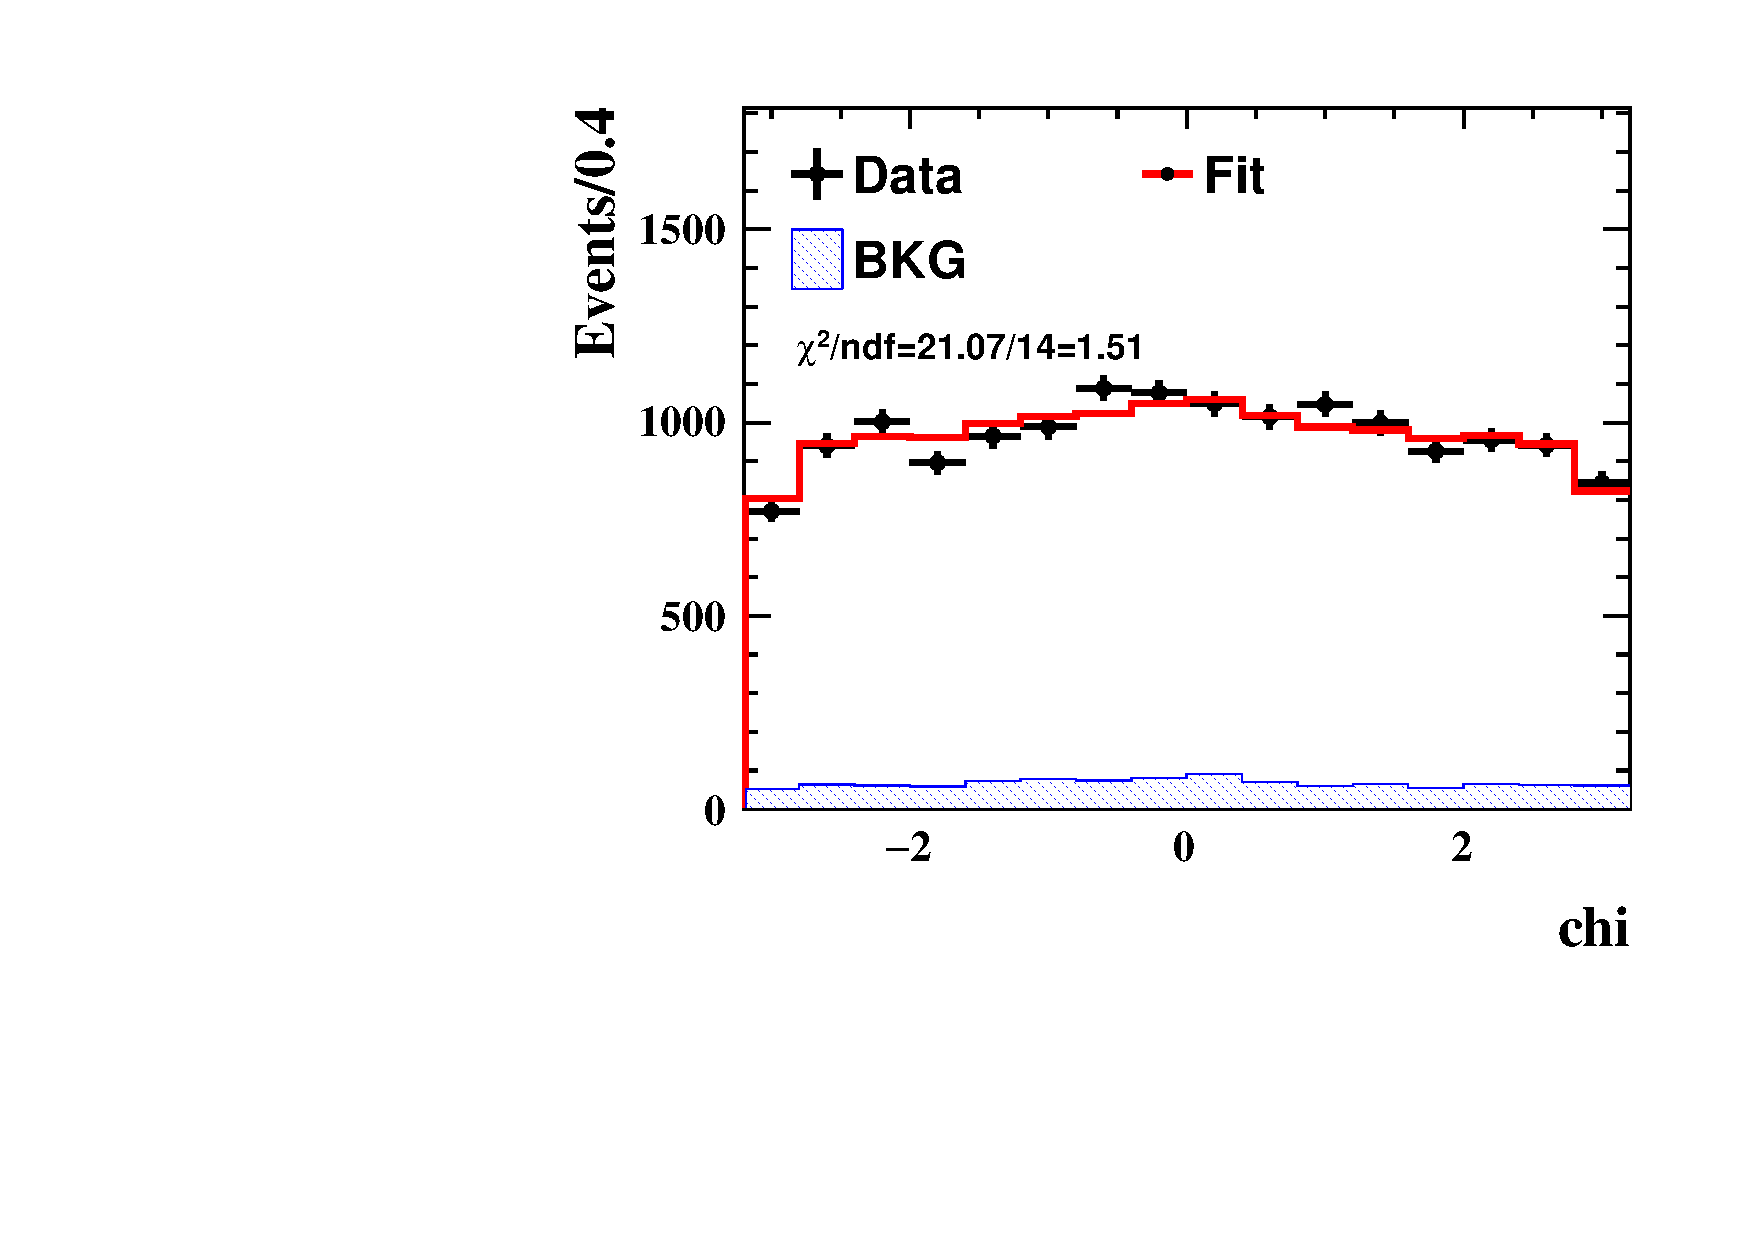
\includegraphics[width=0.24\textwidth]{figure/polarimetery/angular_plots/pkpi_4680_phi2.pdf}
    \caption{Fit results of helicity angles of $\theta_{\lcp}$, $\theta$, $\phi$ and $\chi$ at $\sqrt{s} = 4.682\gev/c^2$.}
\label{fig:fit_angular_s5}
\end{figure}

\begin{figure}[H]\centering
    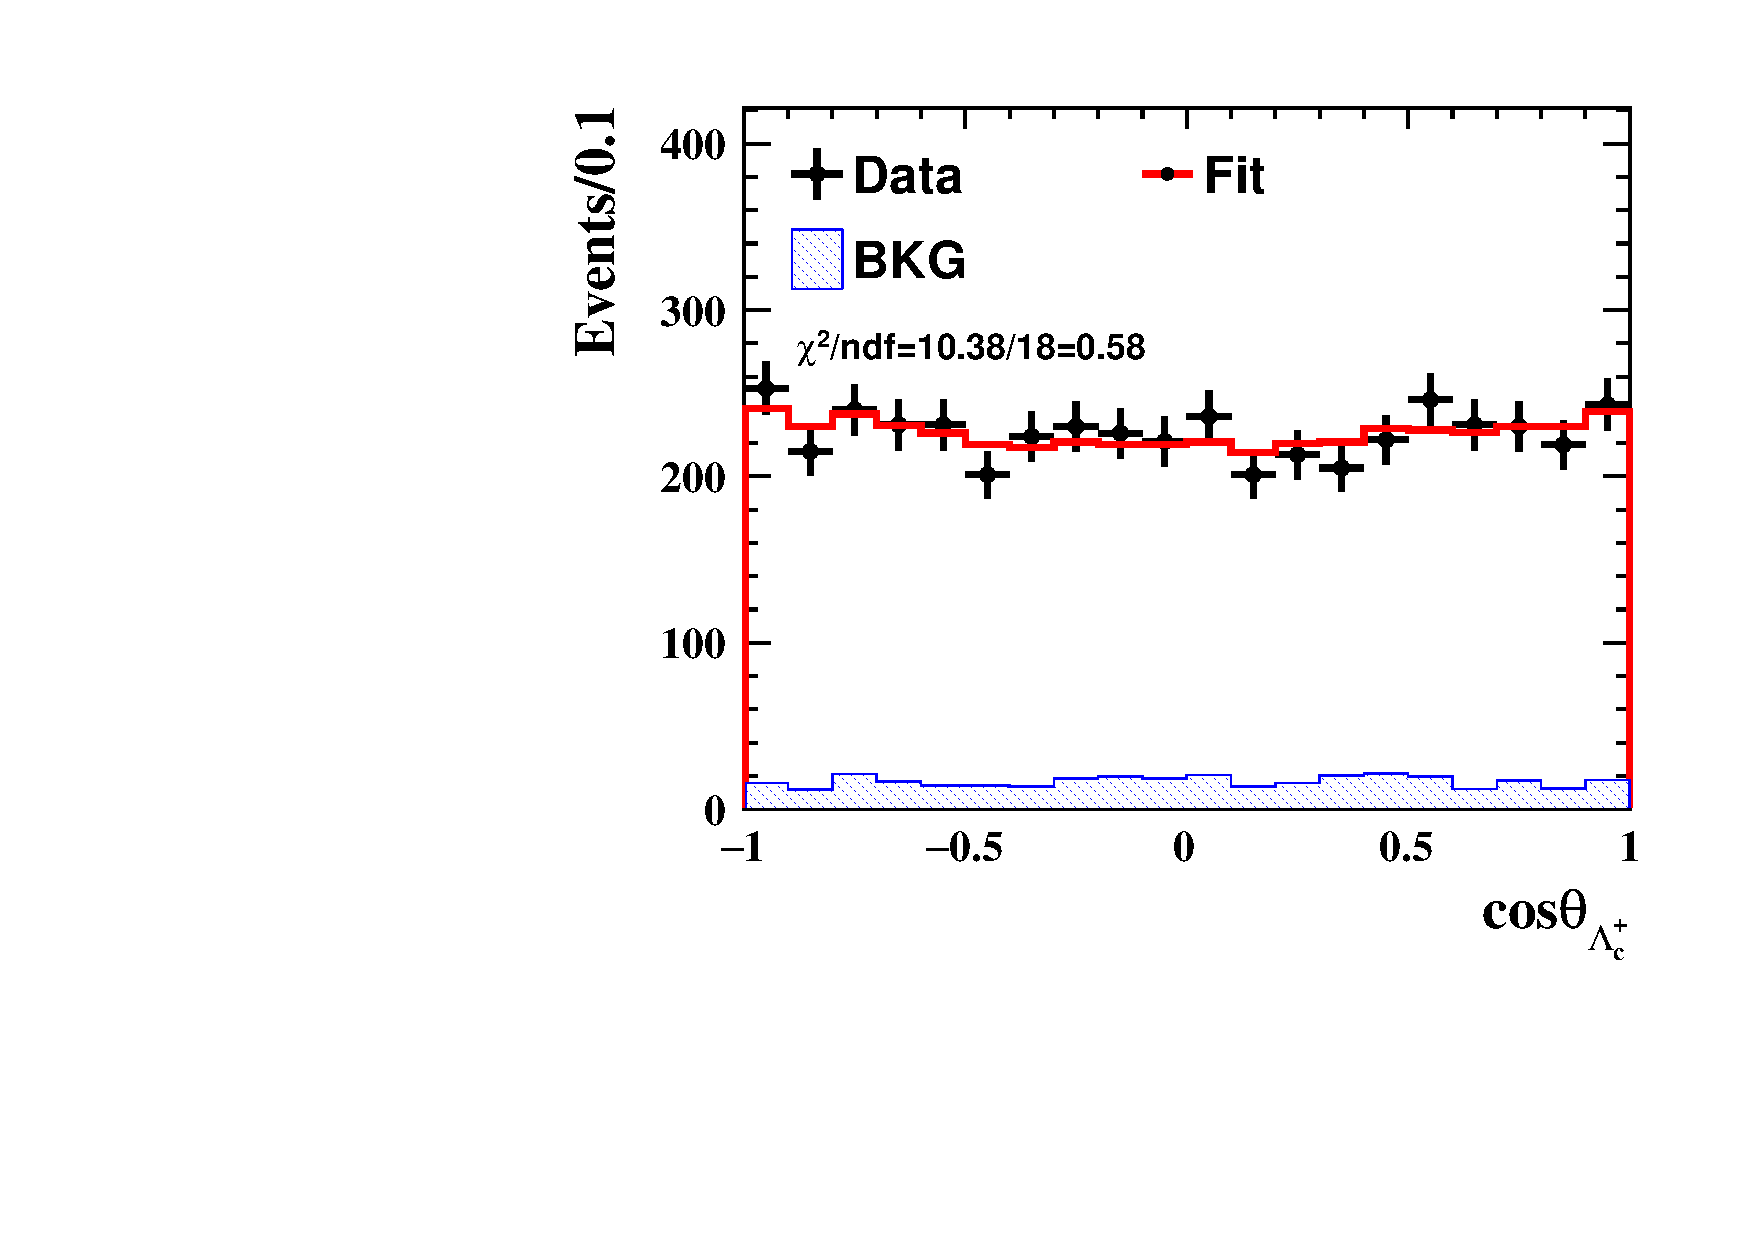
\includegraphics[width=0.24\textwidth]{figure/polarimetery/angular_plots/pkpi_4700_cos_theta0.pdf}
    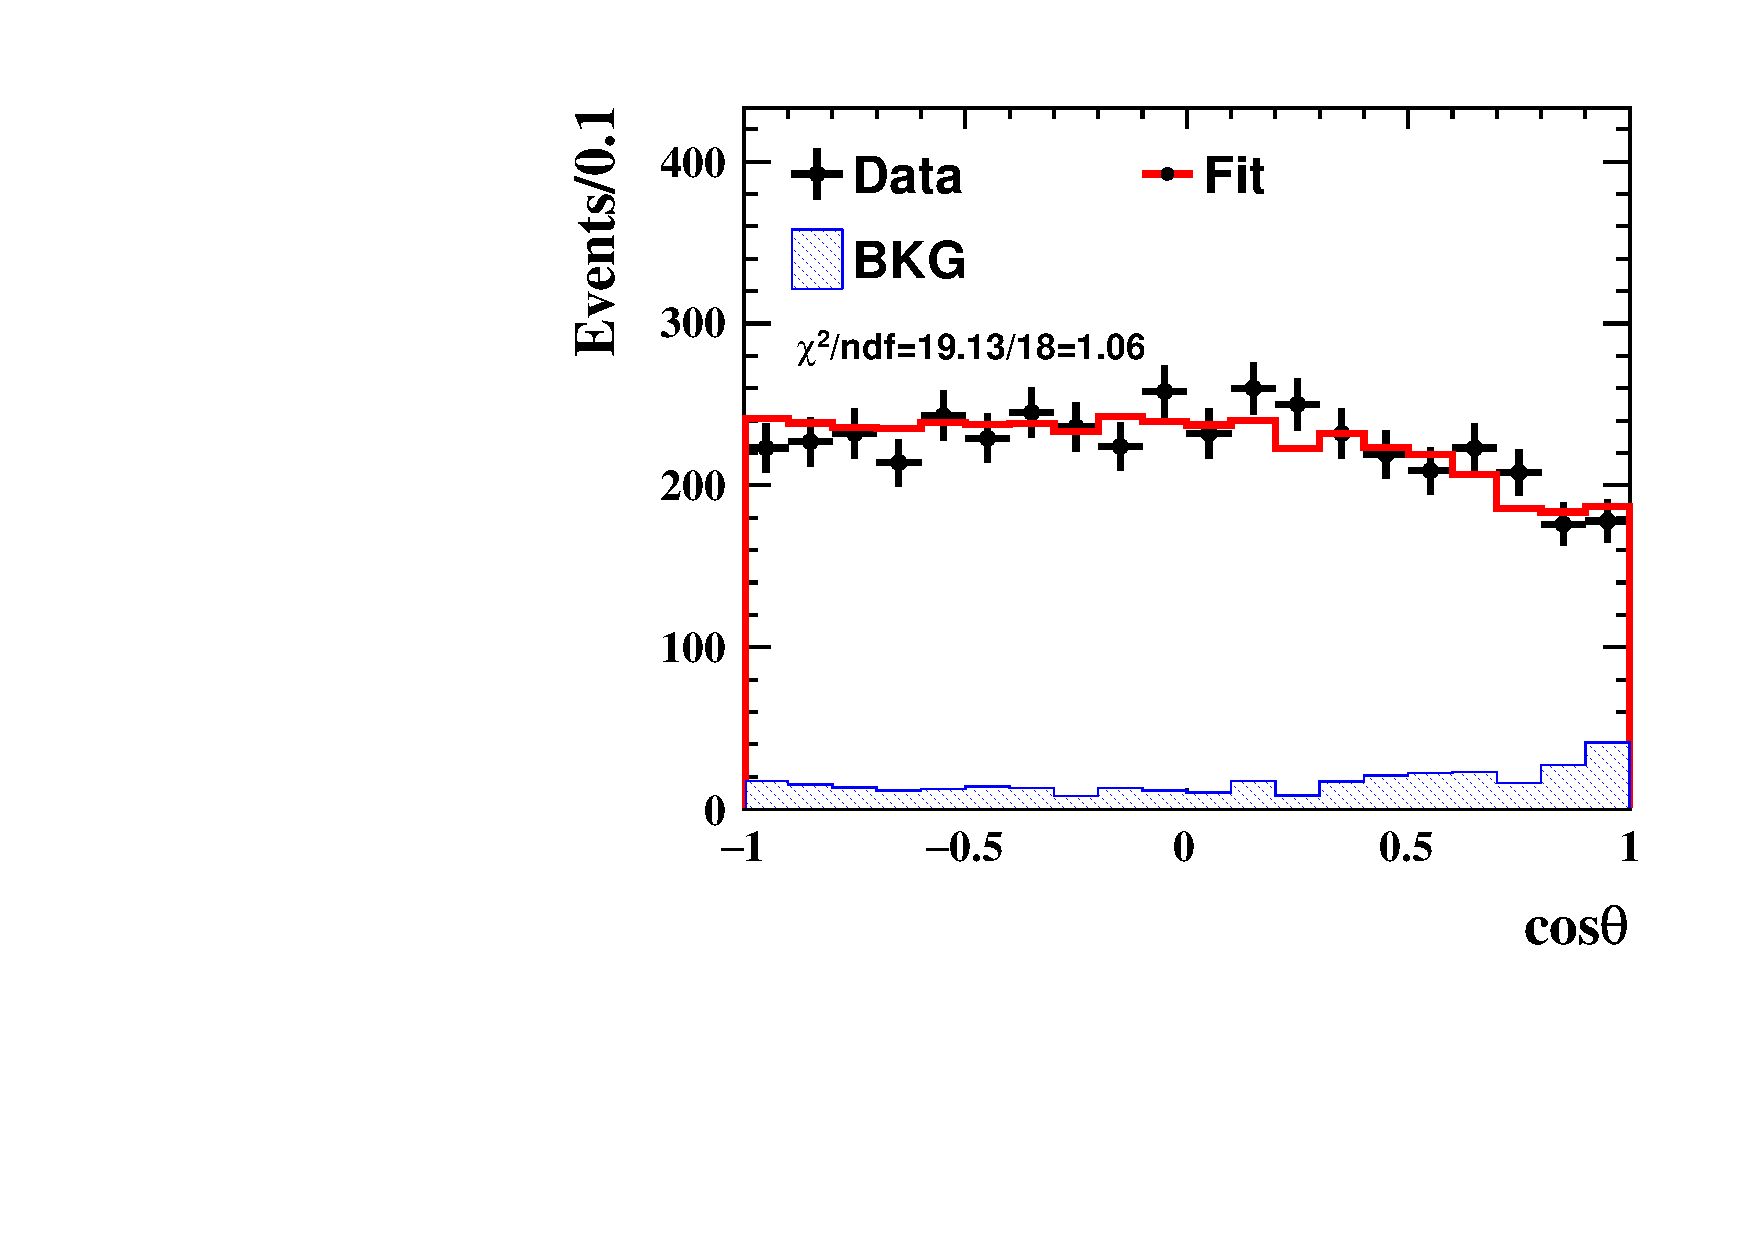
\includegraphics[width=0.24\textwidth]{figure/polarimetery/angular_plots/pkpi_4700_cos_theta1.pdf}
    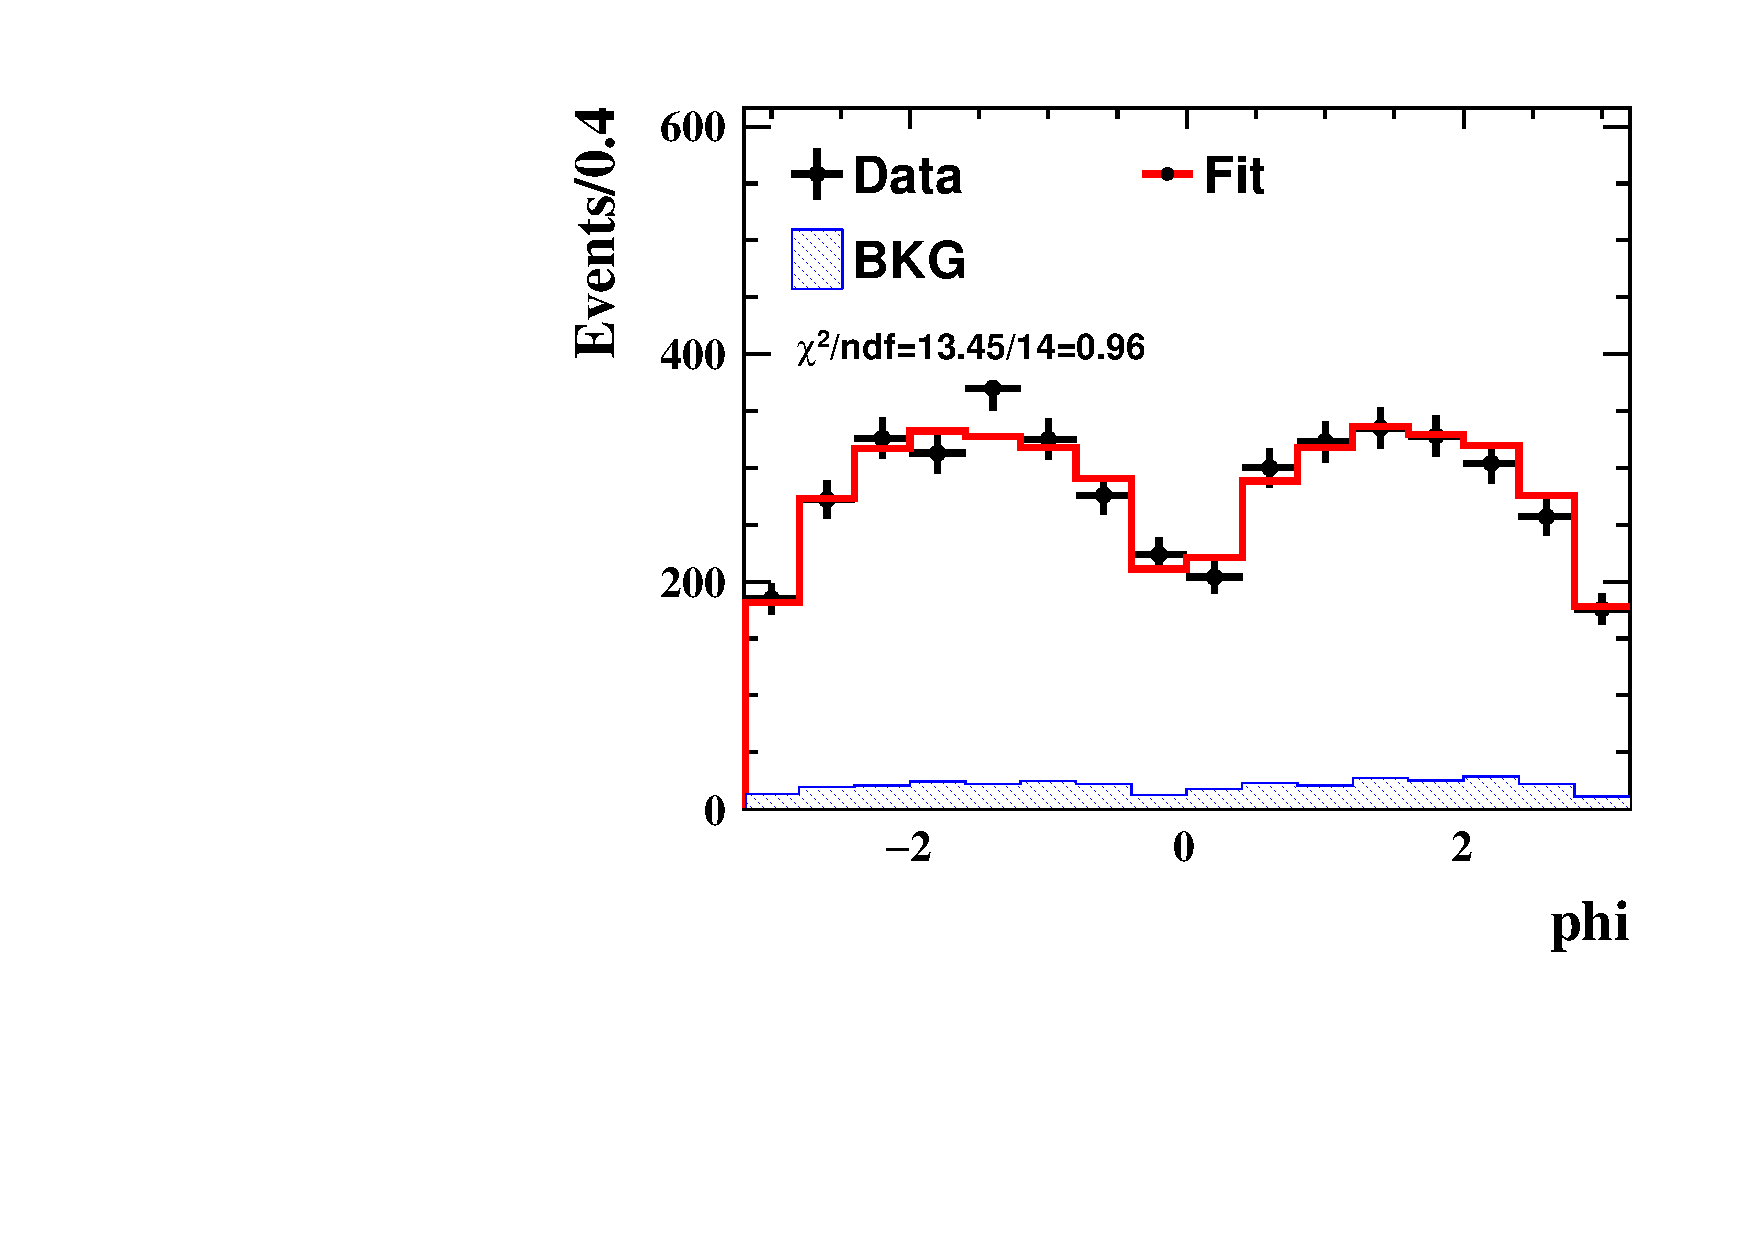
\includegraphics[width=0.24\textwidth]{figure/polarimetery/angular_plots/pkpi_4700_phi1.pdf}
    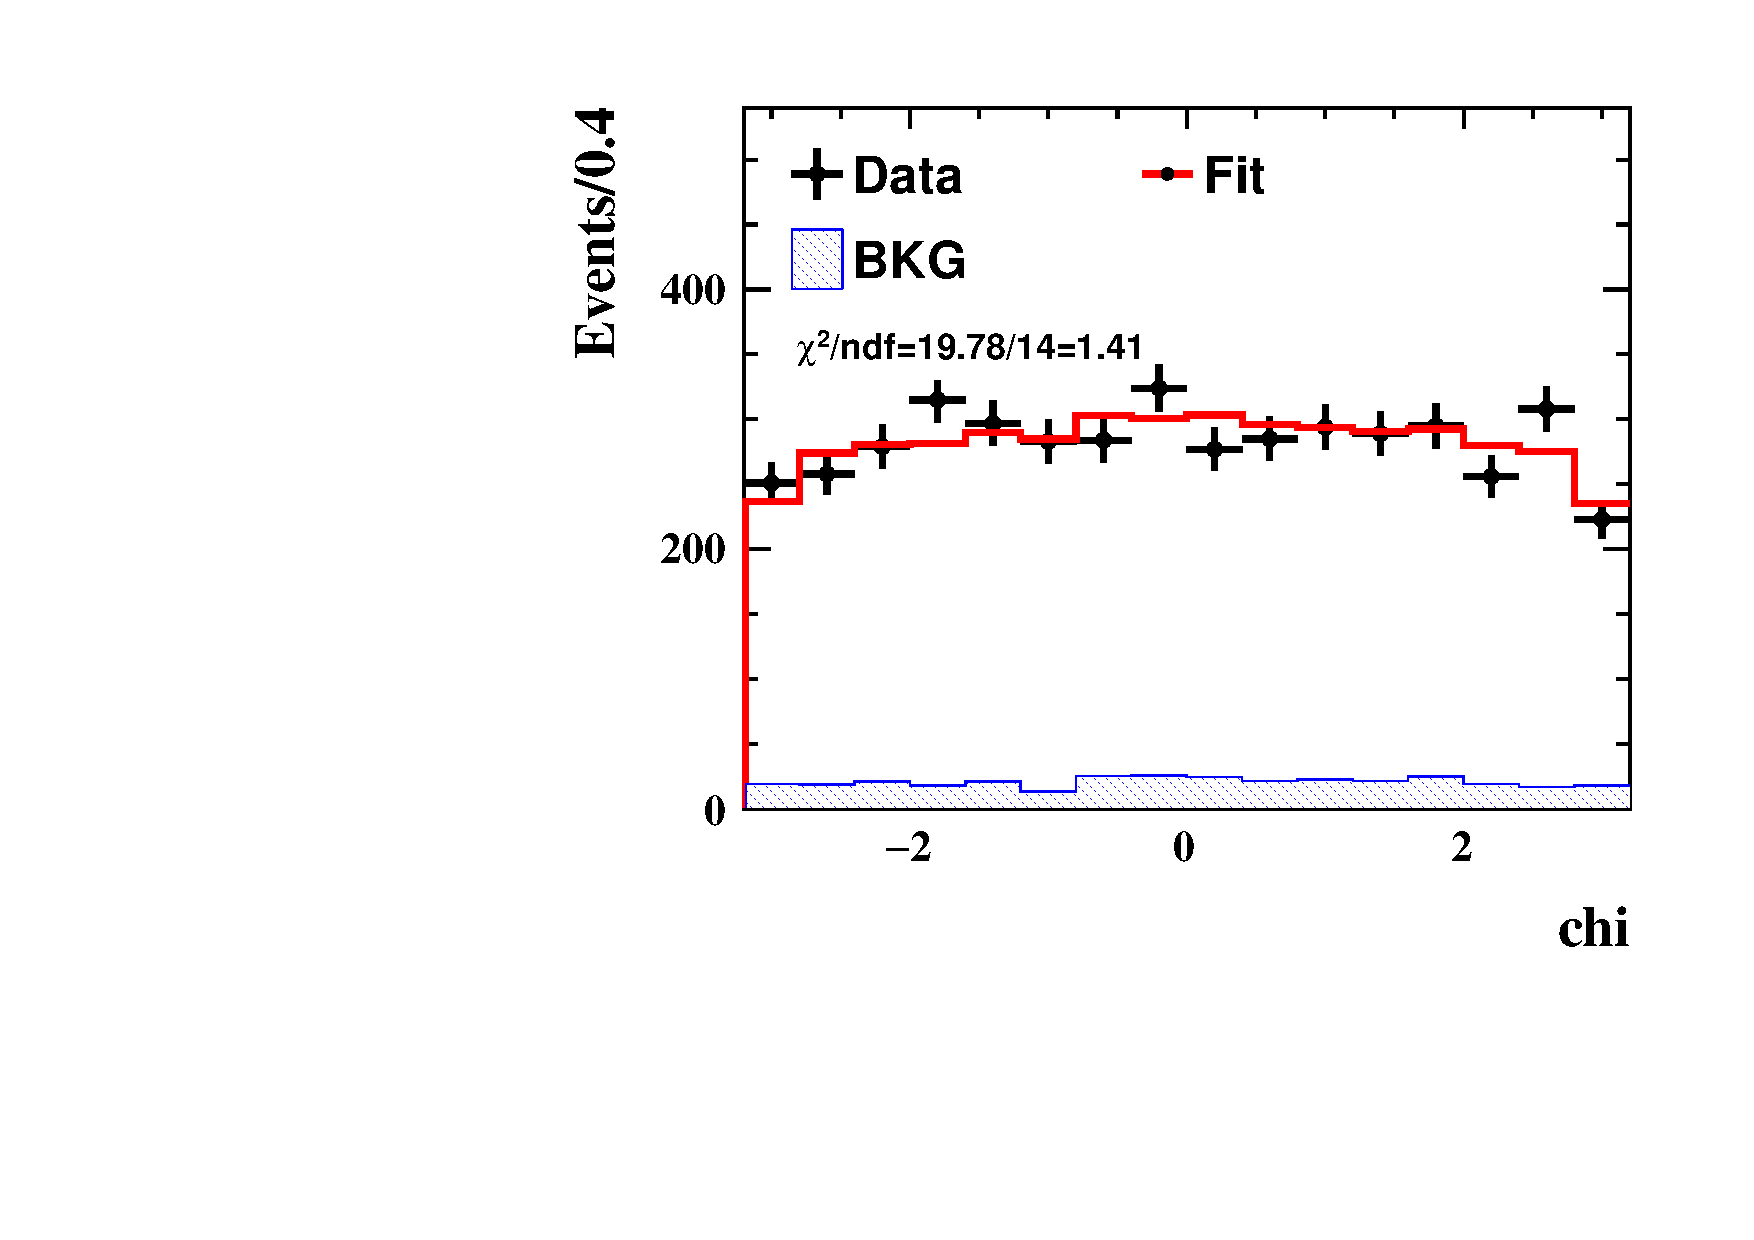
\includegraphics[width=0.24\textwidth]{figure/polarimetery/angular_plots/pkpi_4700_phi2.pdf}
    \caption{Fit results of helicity angles of $\theta_{\lcp}$, $\theta$, $\phi$ and $\chi$ at $\sqrt{s} = 4.699\gev/c^2$.}
\label{fig:fit_angular_s6}
\end{figure}

\begin{figure}[H]\centering
    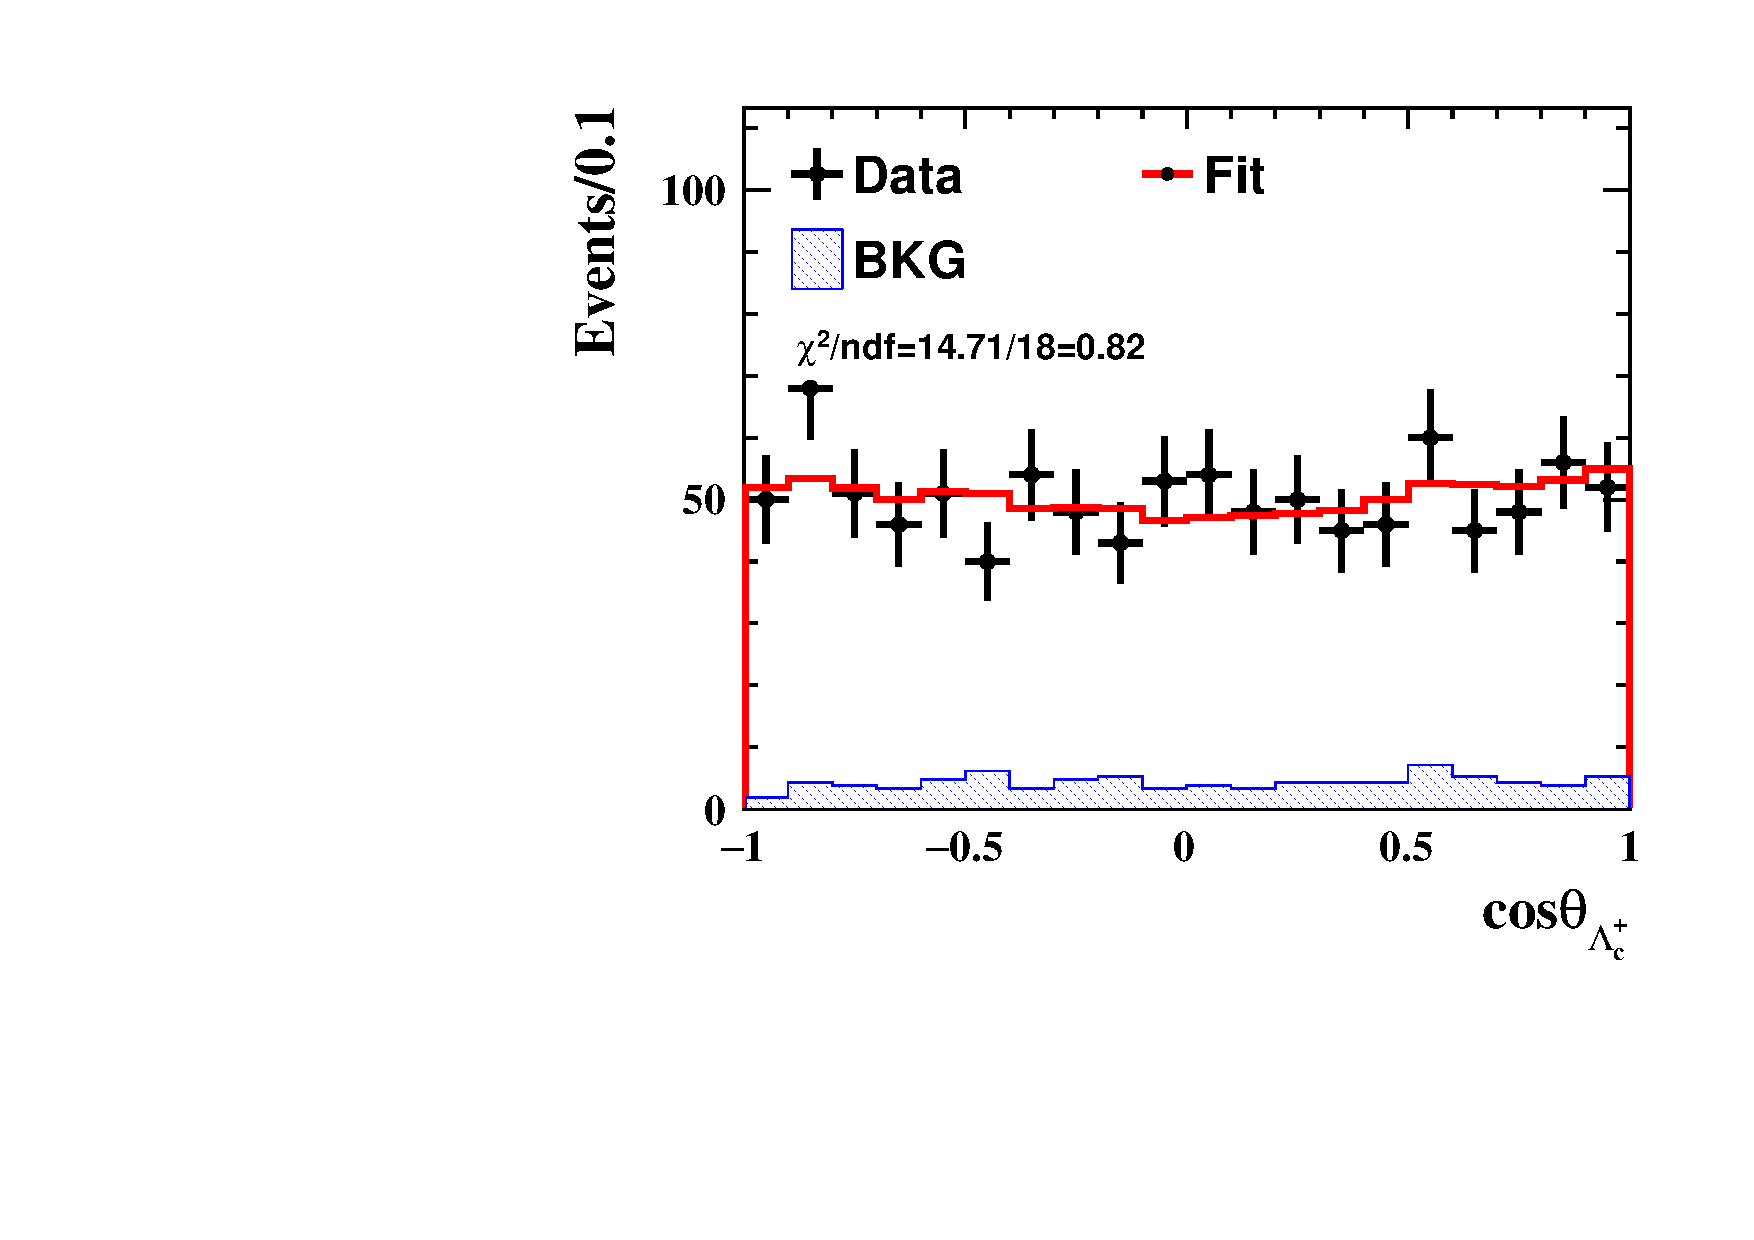
\includegraphics[width=0.24\textwidth]{figure/polarimetery/angular_plots/pkpi_4740_cos_theta0.pdf}
    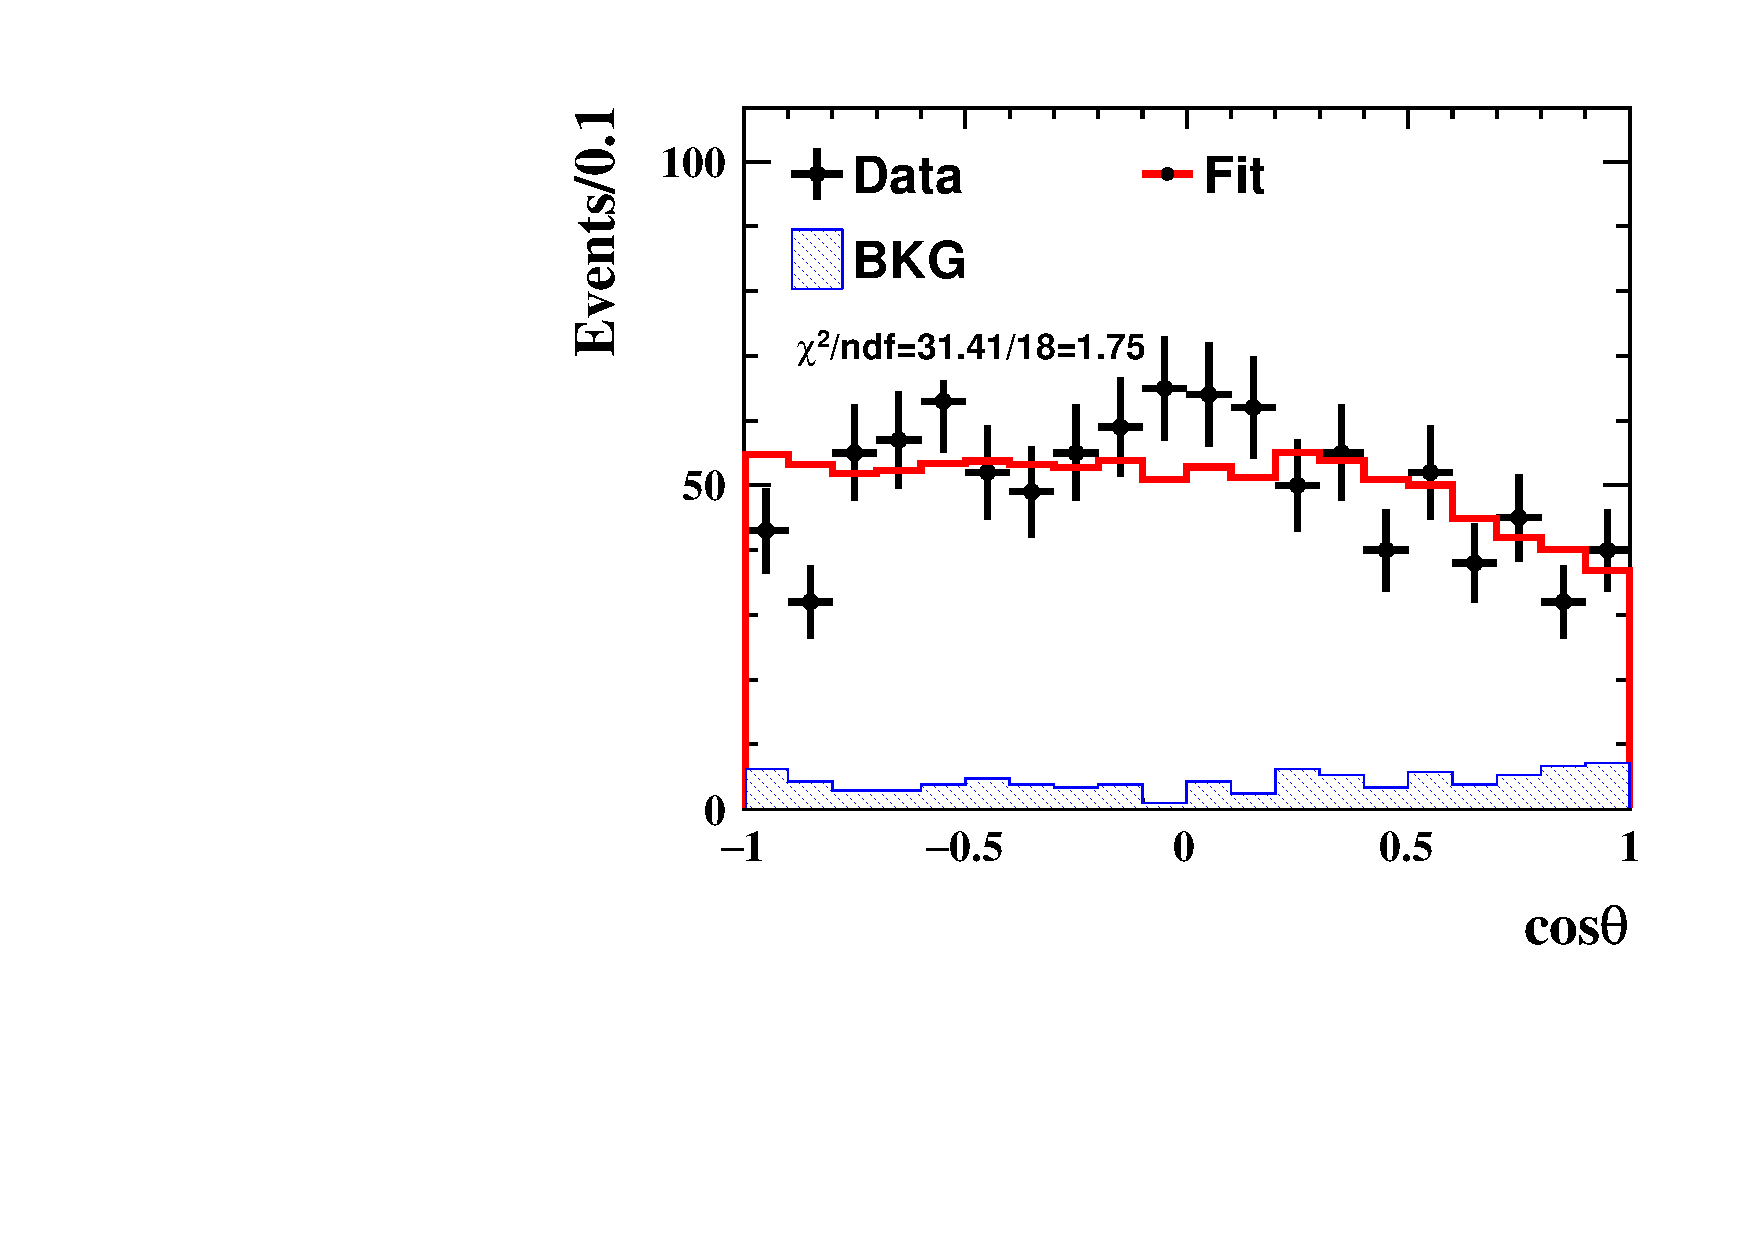
\includegraphics[width=0.24\textwidth]{figure/polarimetery/angular_plots/pkpi_4740_cos_theta1.pdf}
    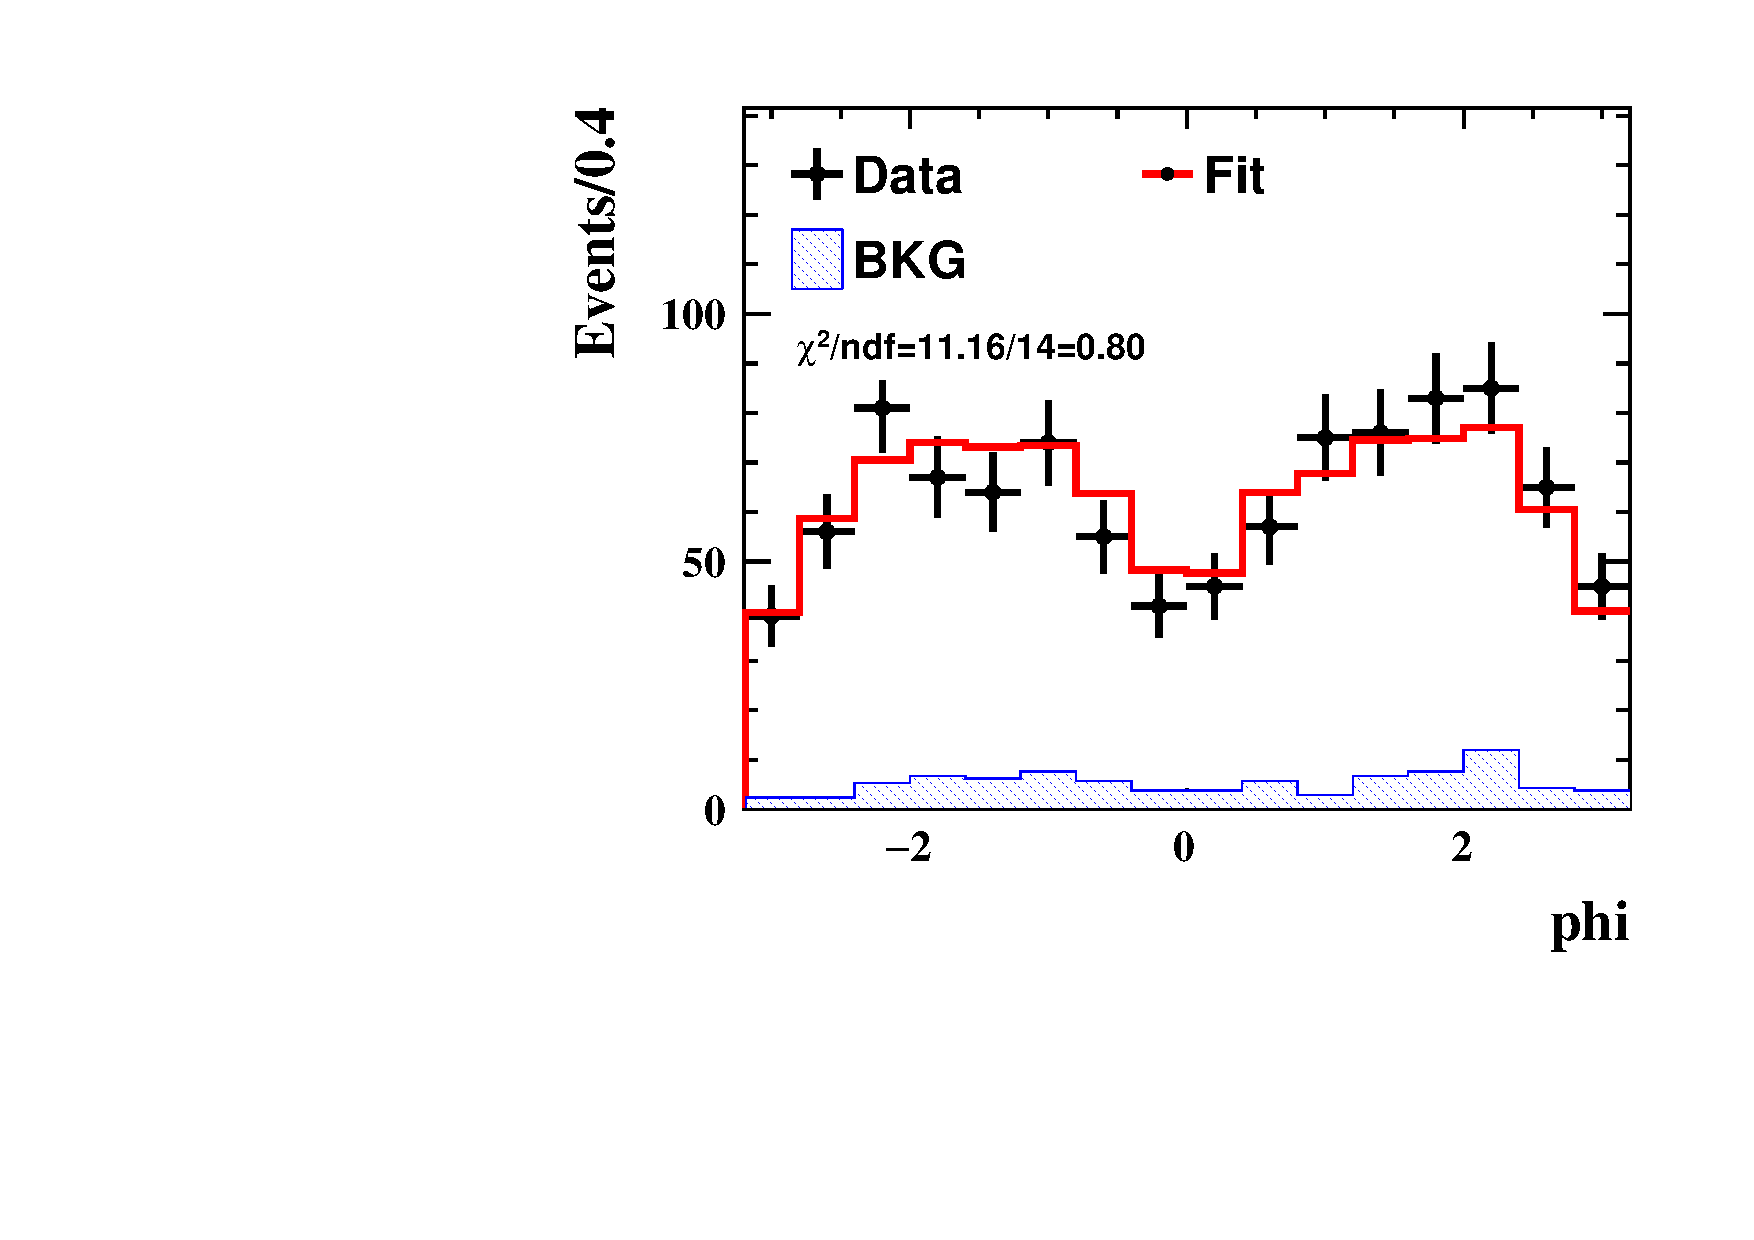
\includegraphics[width=0.24\textwidth]{figure/polarimetery/angular_plots/pkpi_4740_phi1.pdf}
    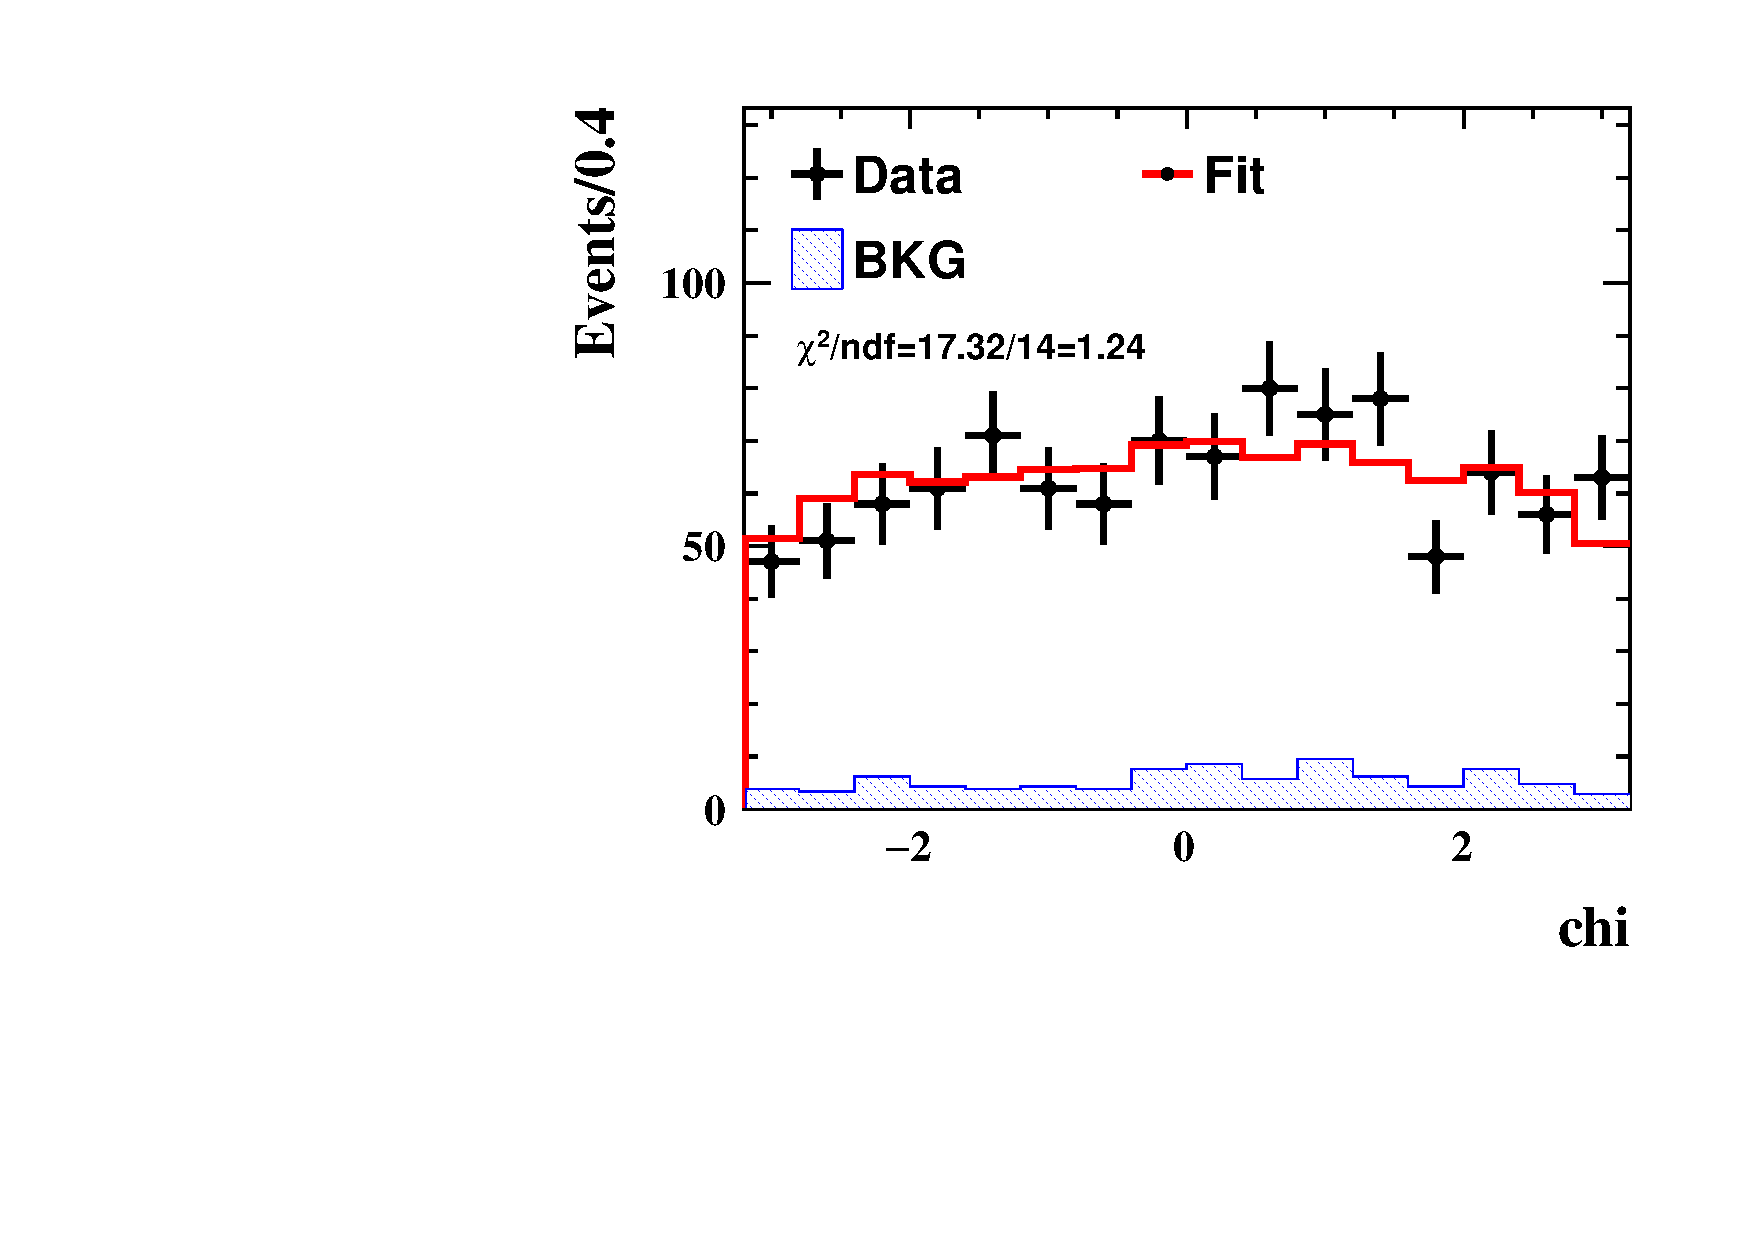
\includegraphics[width=0.24\textwidth]{figure/polarimetery/angular_plots/pkpi_4740_phi2.pdf}
    \caption{Fit results of helicity angles of $\theta_{\lcp}$, $\theta$, $\phi$ and $\chi$ at $\sqrt{s} = 4.740\gev/c^2$.}
\label{fig:fit_angular_s7}
\end{figure}

\begin{figure}[H]\centering
    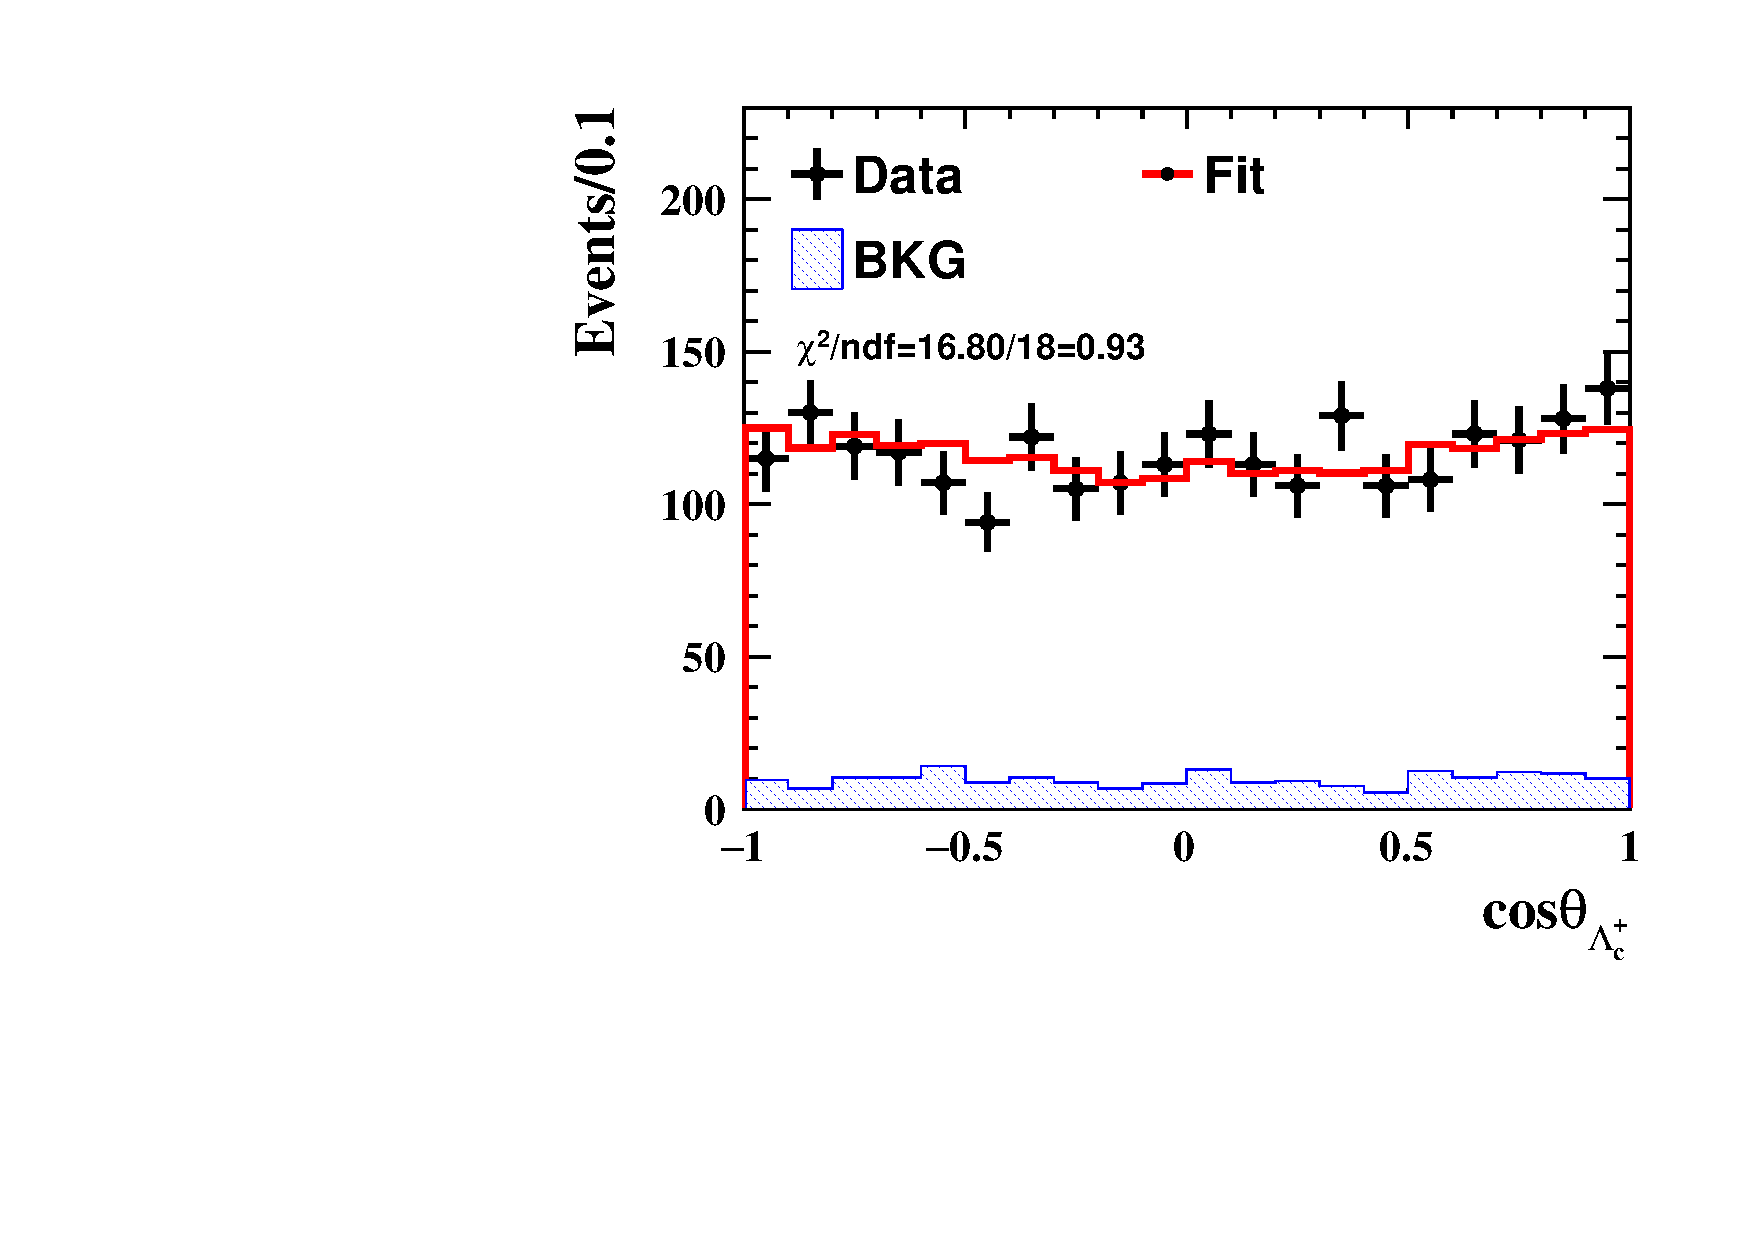
\includegraphics[width=0.24\textwidth]{figure/polarimetery/angular_plots/pkpi_4750_cos_theta0.pdf}
    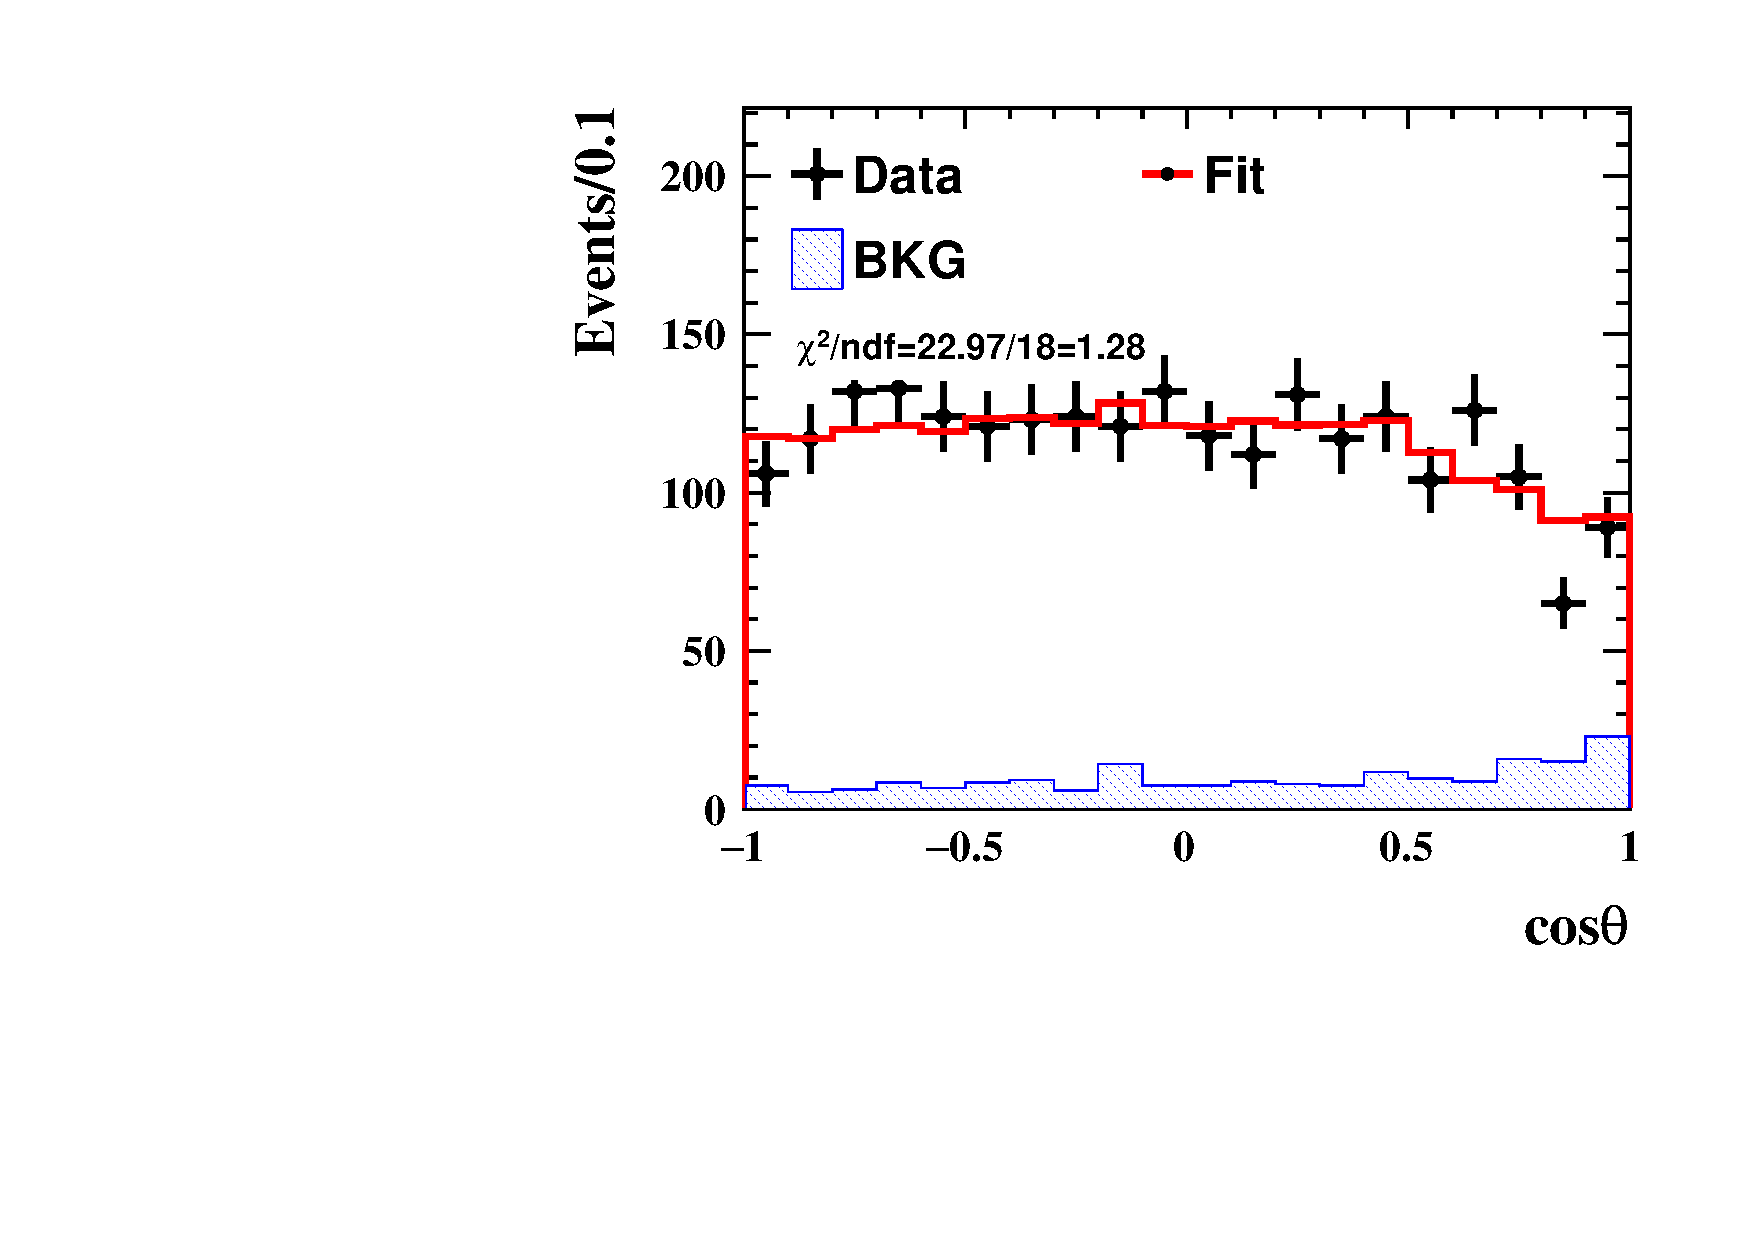
\includegraphics[width=0.24\textwidth]{figure/polarimetery/angular_plots/pkpi_4750_cos_theta1.pdf}
    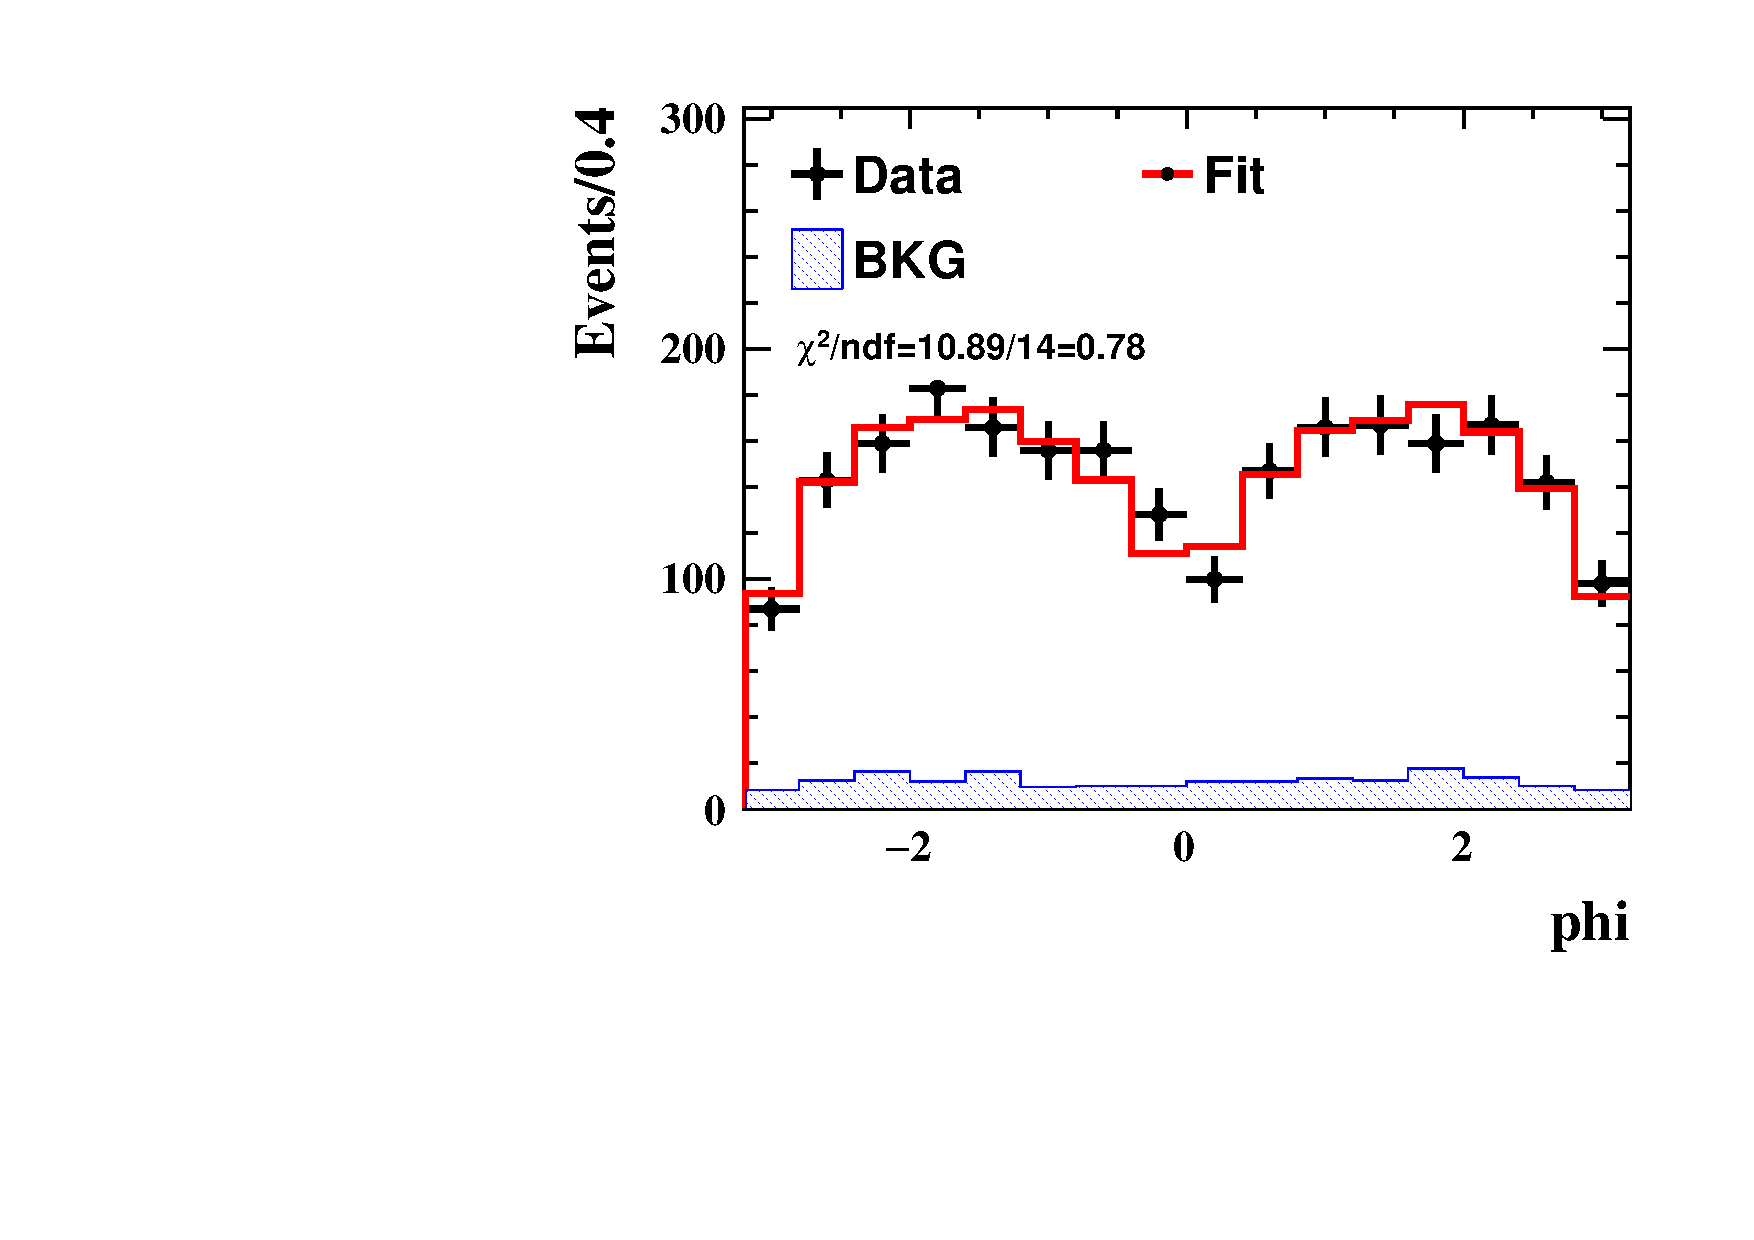
\includegraphics[width=0.24\textwidth]{figure/polarimetery/angular_plots/pkpi_4750_phi1.pdf}
    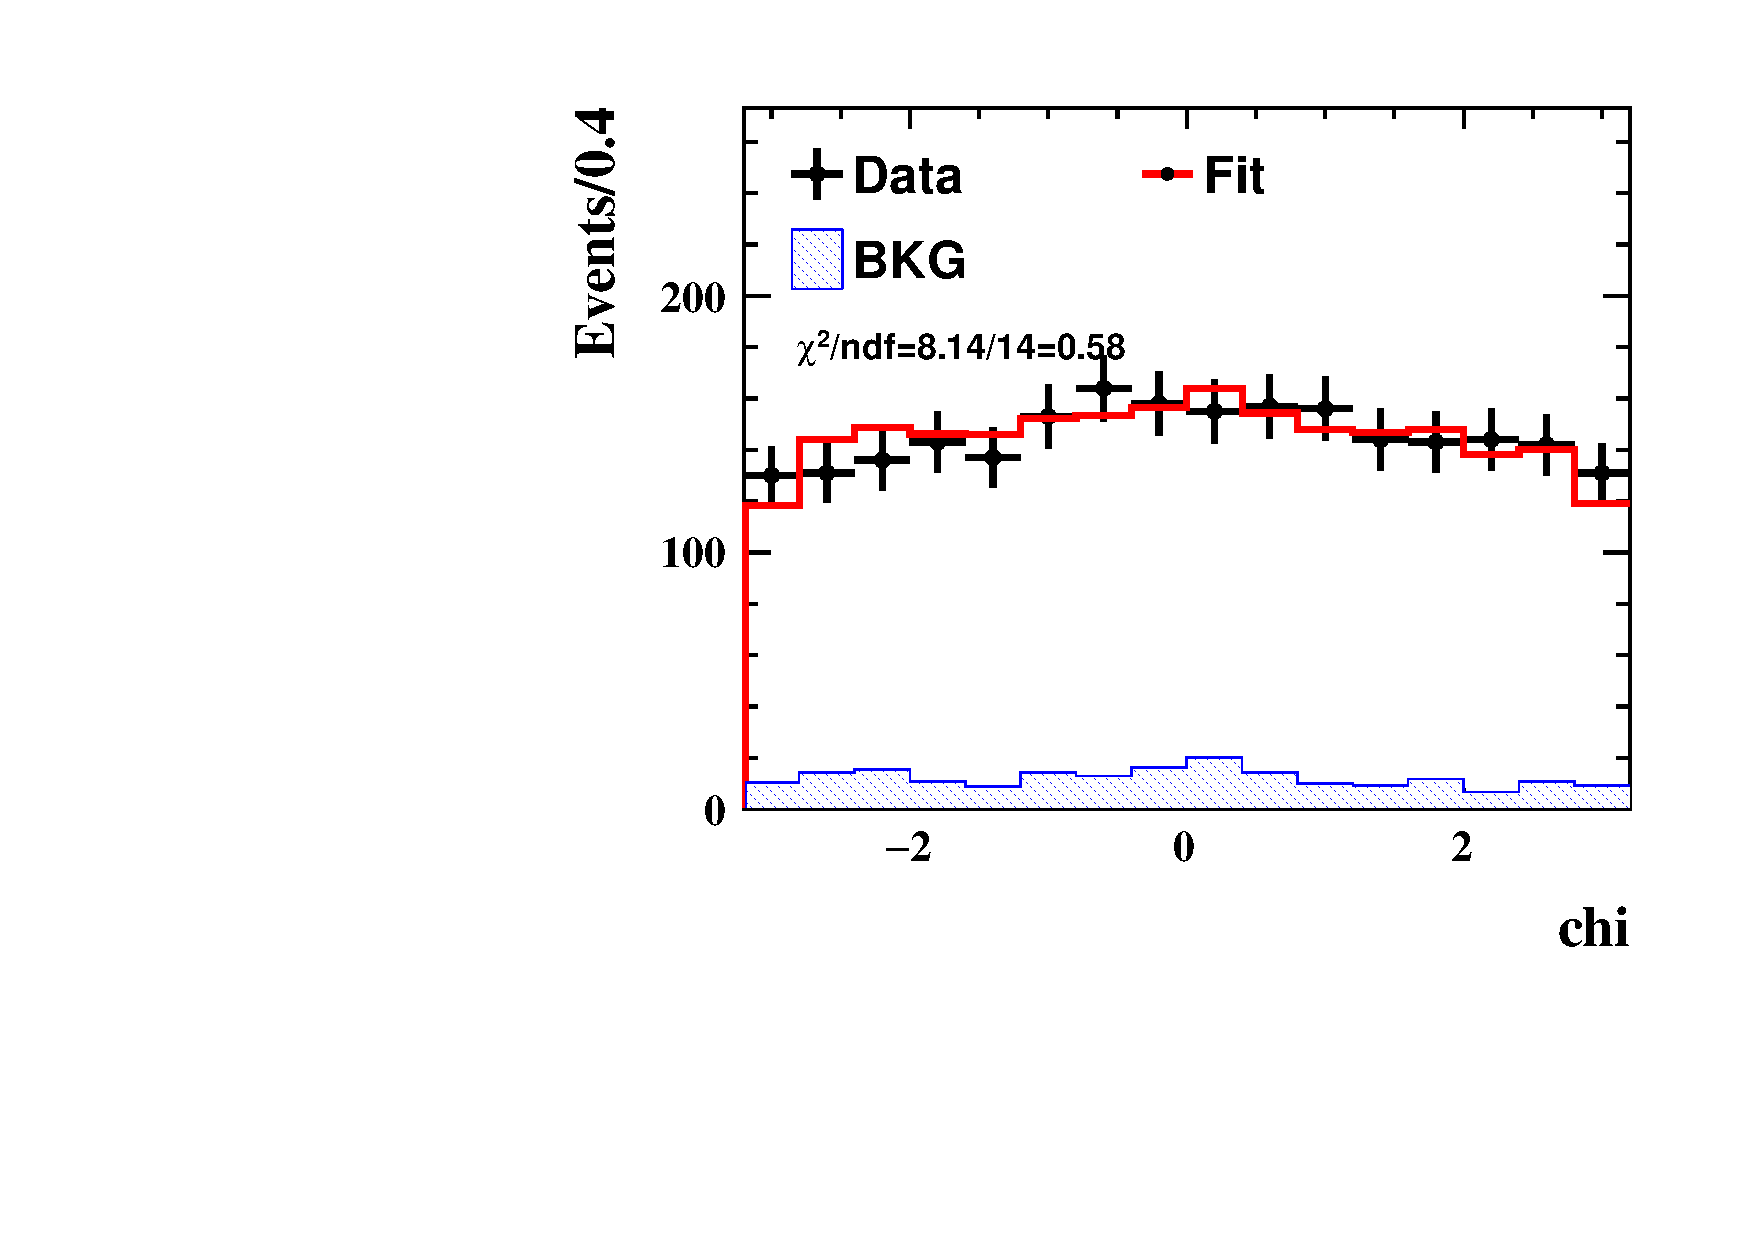
\includegraphics[width=0.24\textwidth]{figure/polarimetery/angular_plots/pkpi_4750_phi2.pdf}
    \caption{Fit results of helicity angles of $\theta_{\lcp}$, $\theta$, $\phi$ and $\chi$ at $\sqrt{s} = 4.750\gev/c^2$.}
\label{fig:fit_angular_s8}
\end{figure}

\begin{figure}[H]\centering
    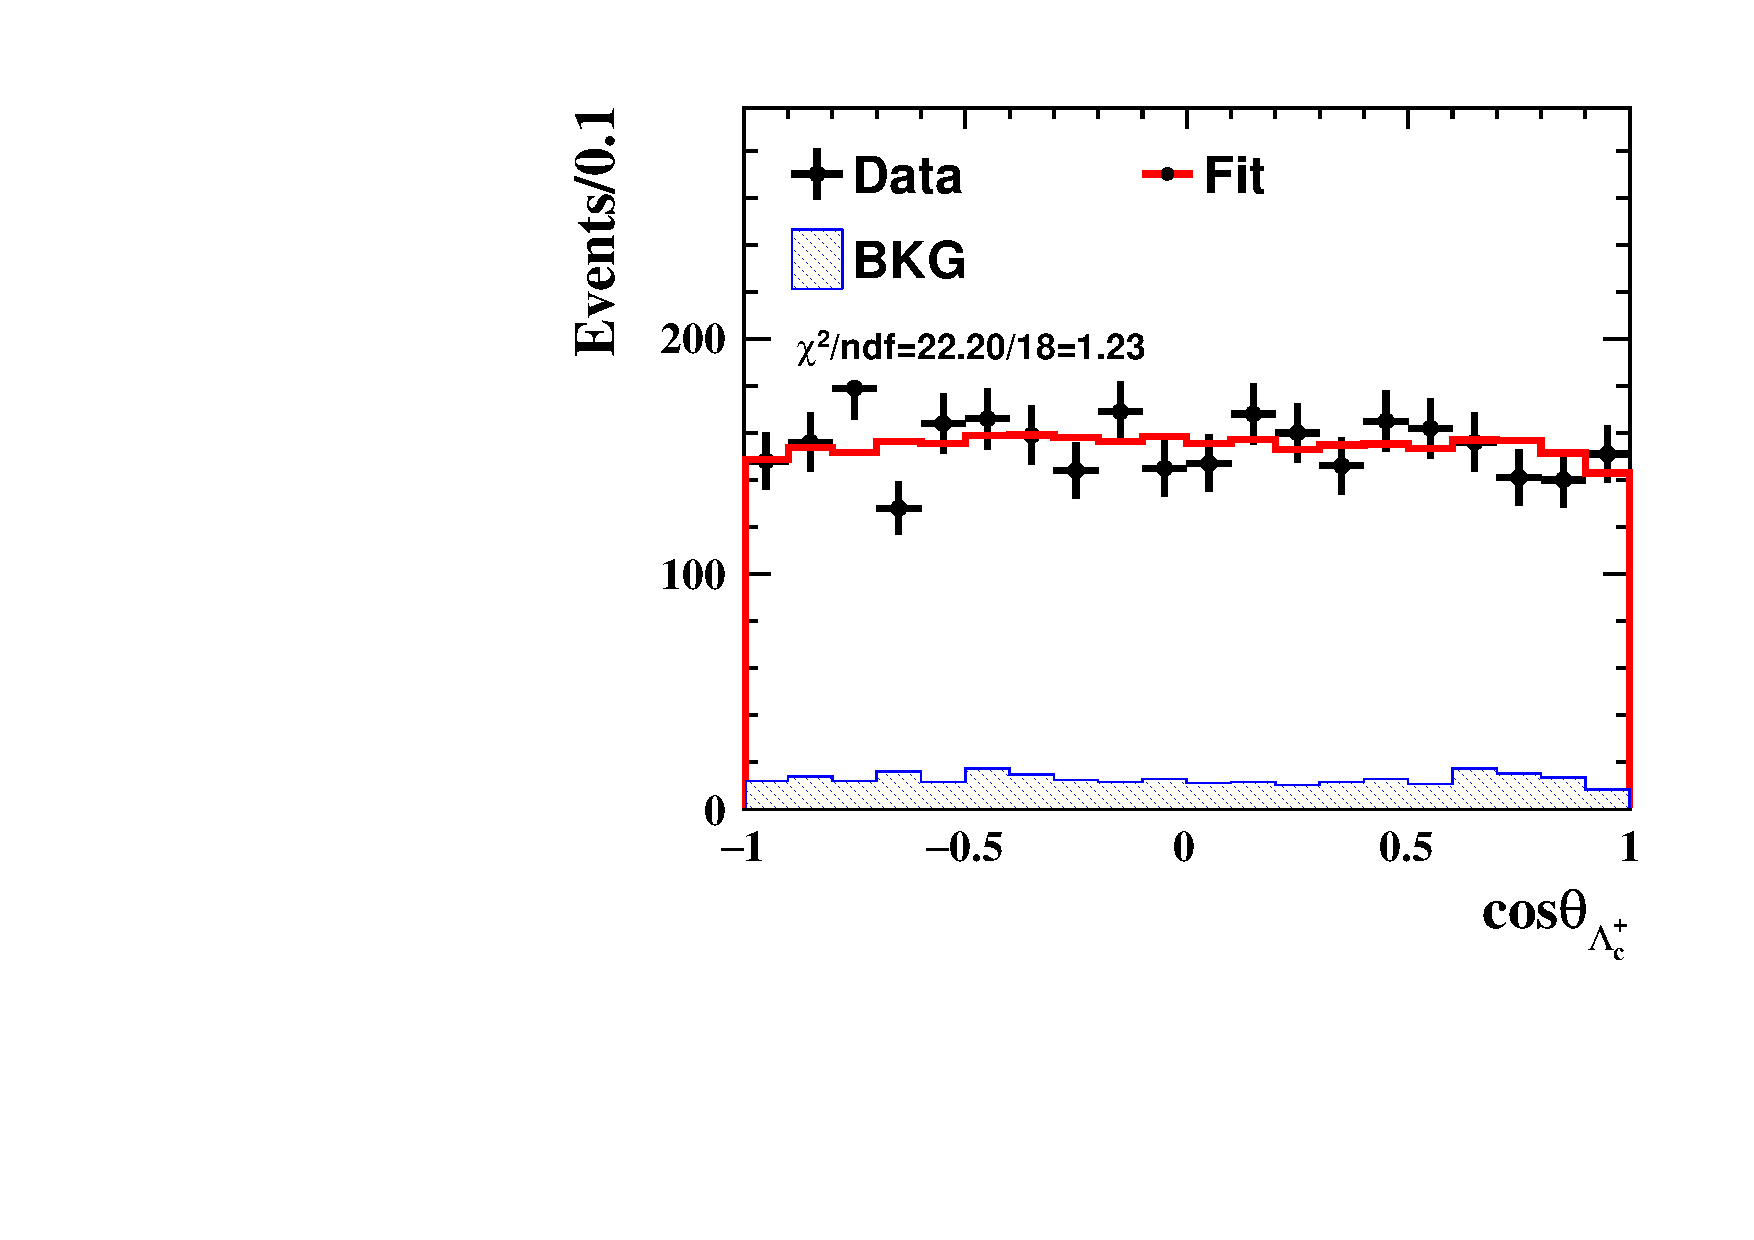
\includegraphics[width=0.24\textwidth]{figure/polarimetery/angular_plots/pkpi_4780_cos_theta0.pdf}
    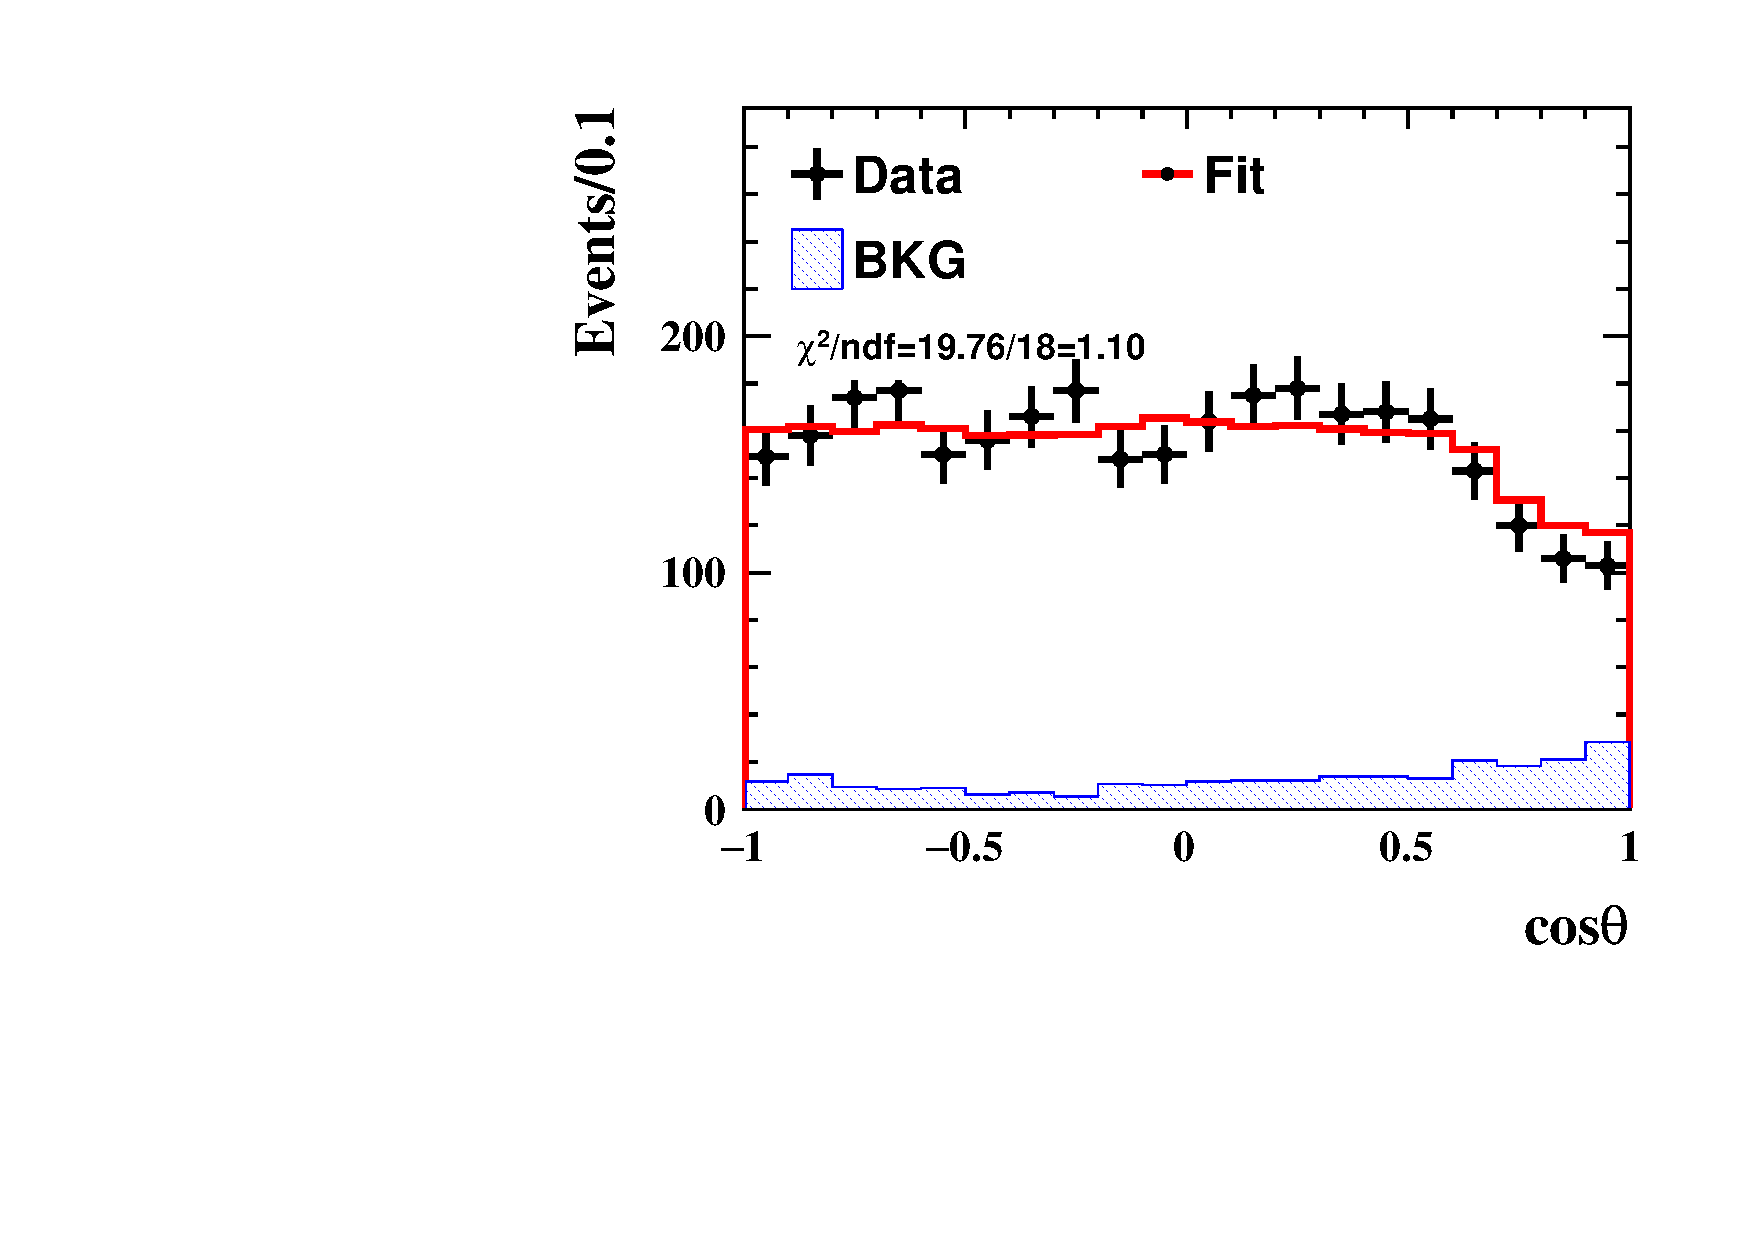
\includegraphics[width=0.24\textwidth]{figure/polarimetery/angular_plots/pkpi_4780_cos_theta1.pdf}
    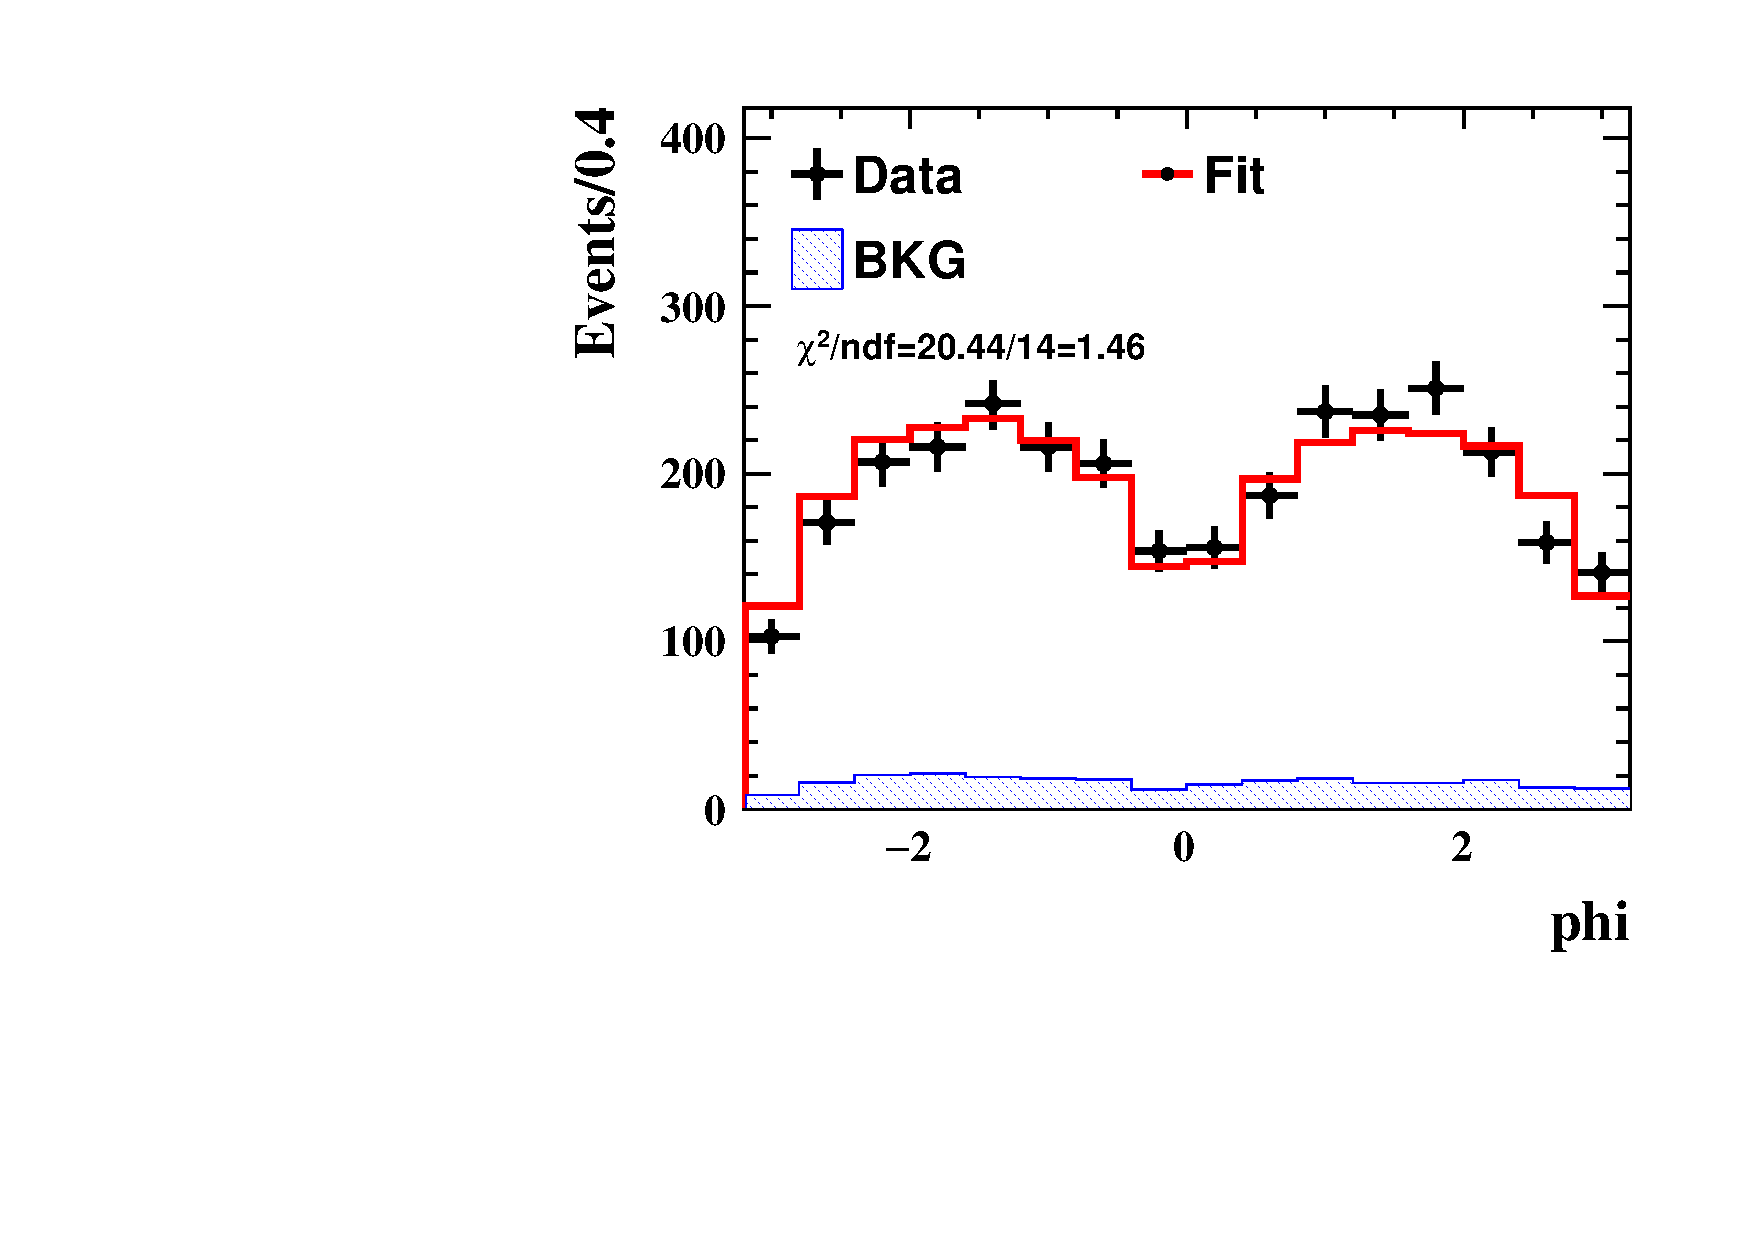
\includegraphics[width=0.24\textwidth]{figure/polarimetery/angular_plots/pkpi_4780_phi1.pdf}
    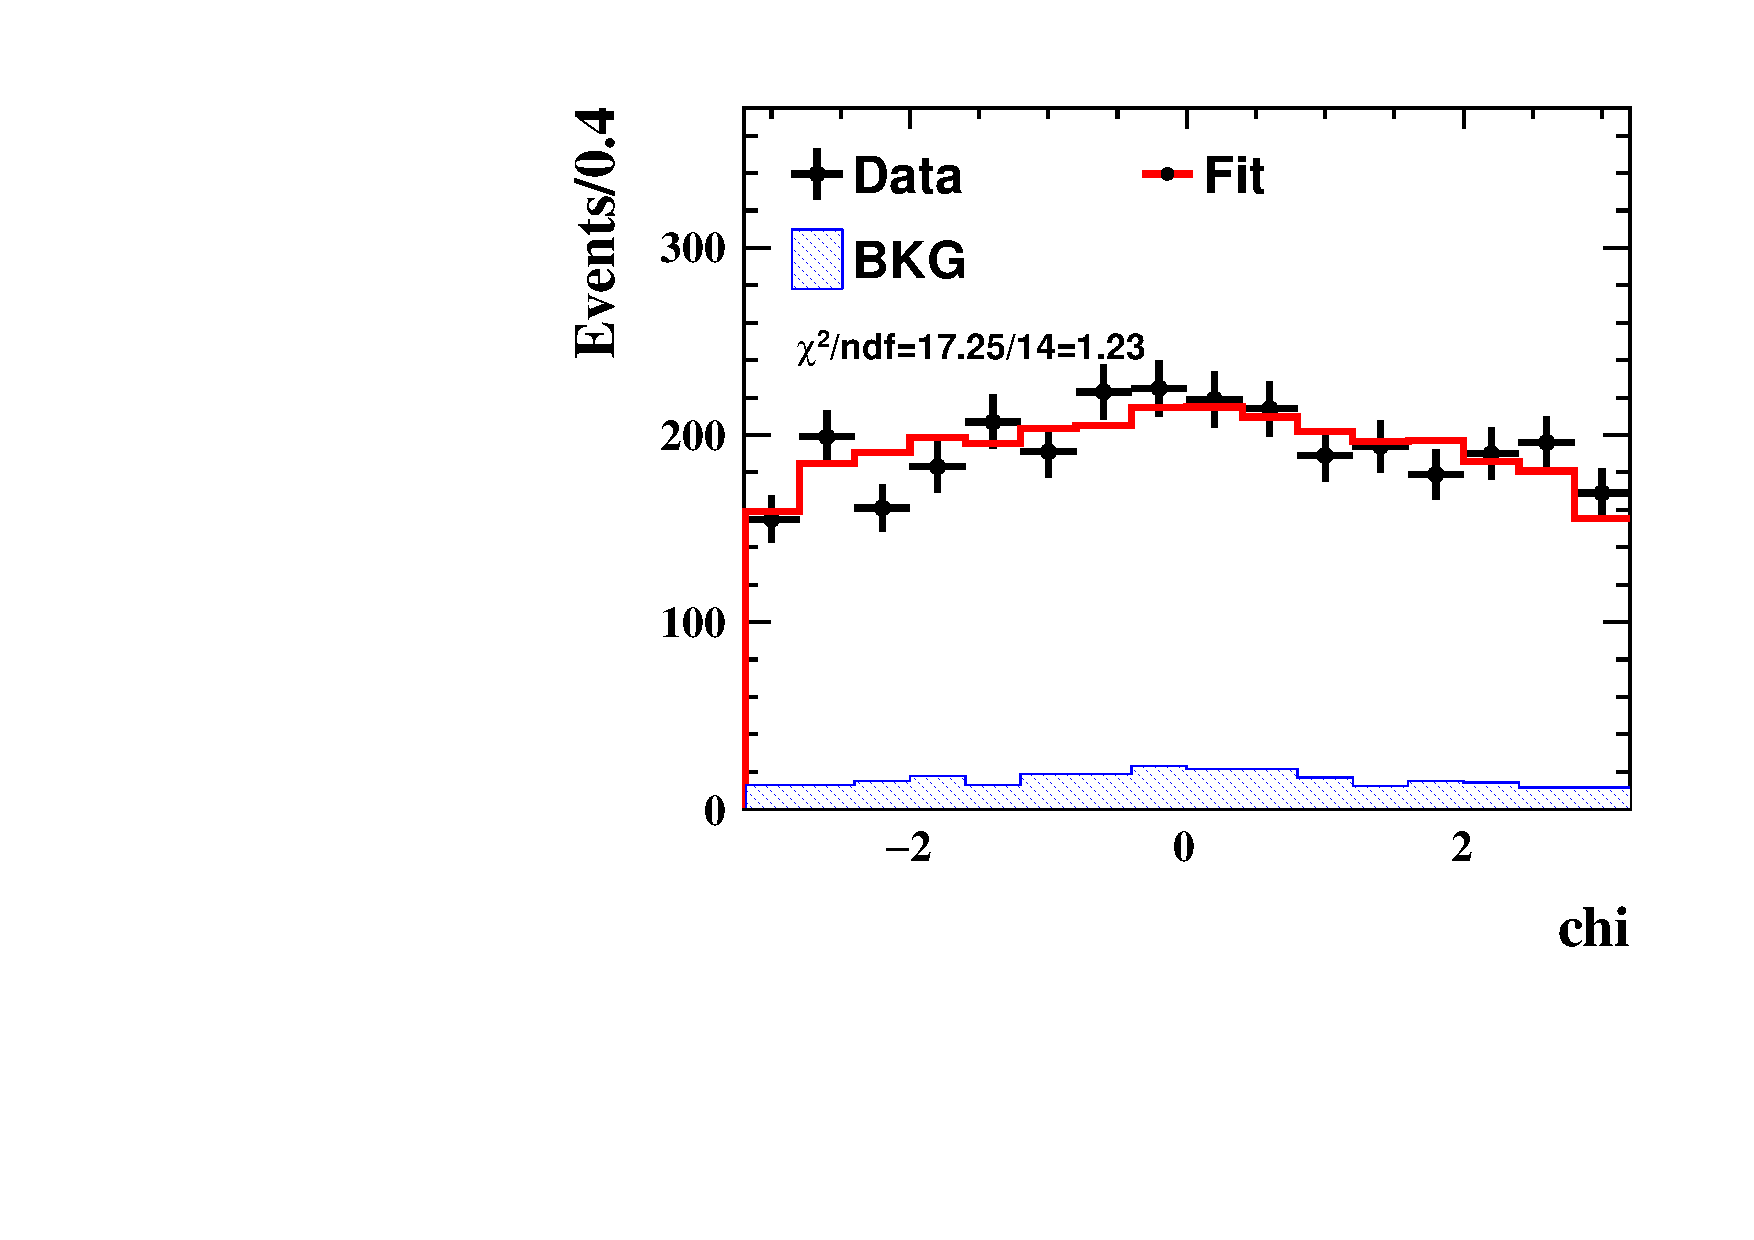
\includegraphics[width=0.24\textwidth]{figure/polarimetery/angular_plots/pkpi_4780_phi2.pdf}
    \caption{Fit results of helicity angles of $\theta_{\lcp}$, $\theta$, $\phi$ and $\chi$ at $\sqrt{s} = 4.781\gev/c^2$.}
\label{fig:fit_angular_s9}
\end{figure}

\begin{figure}[H]\centering
    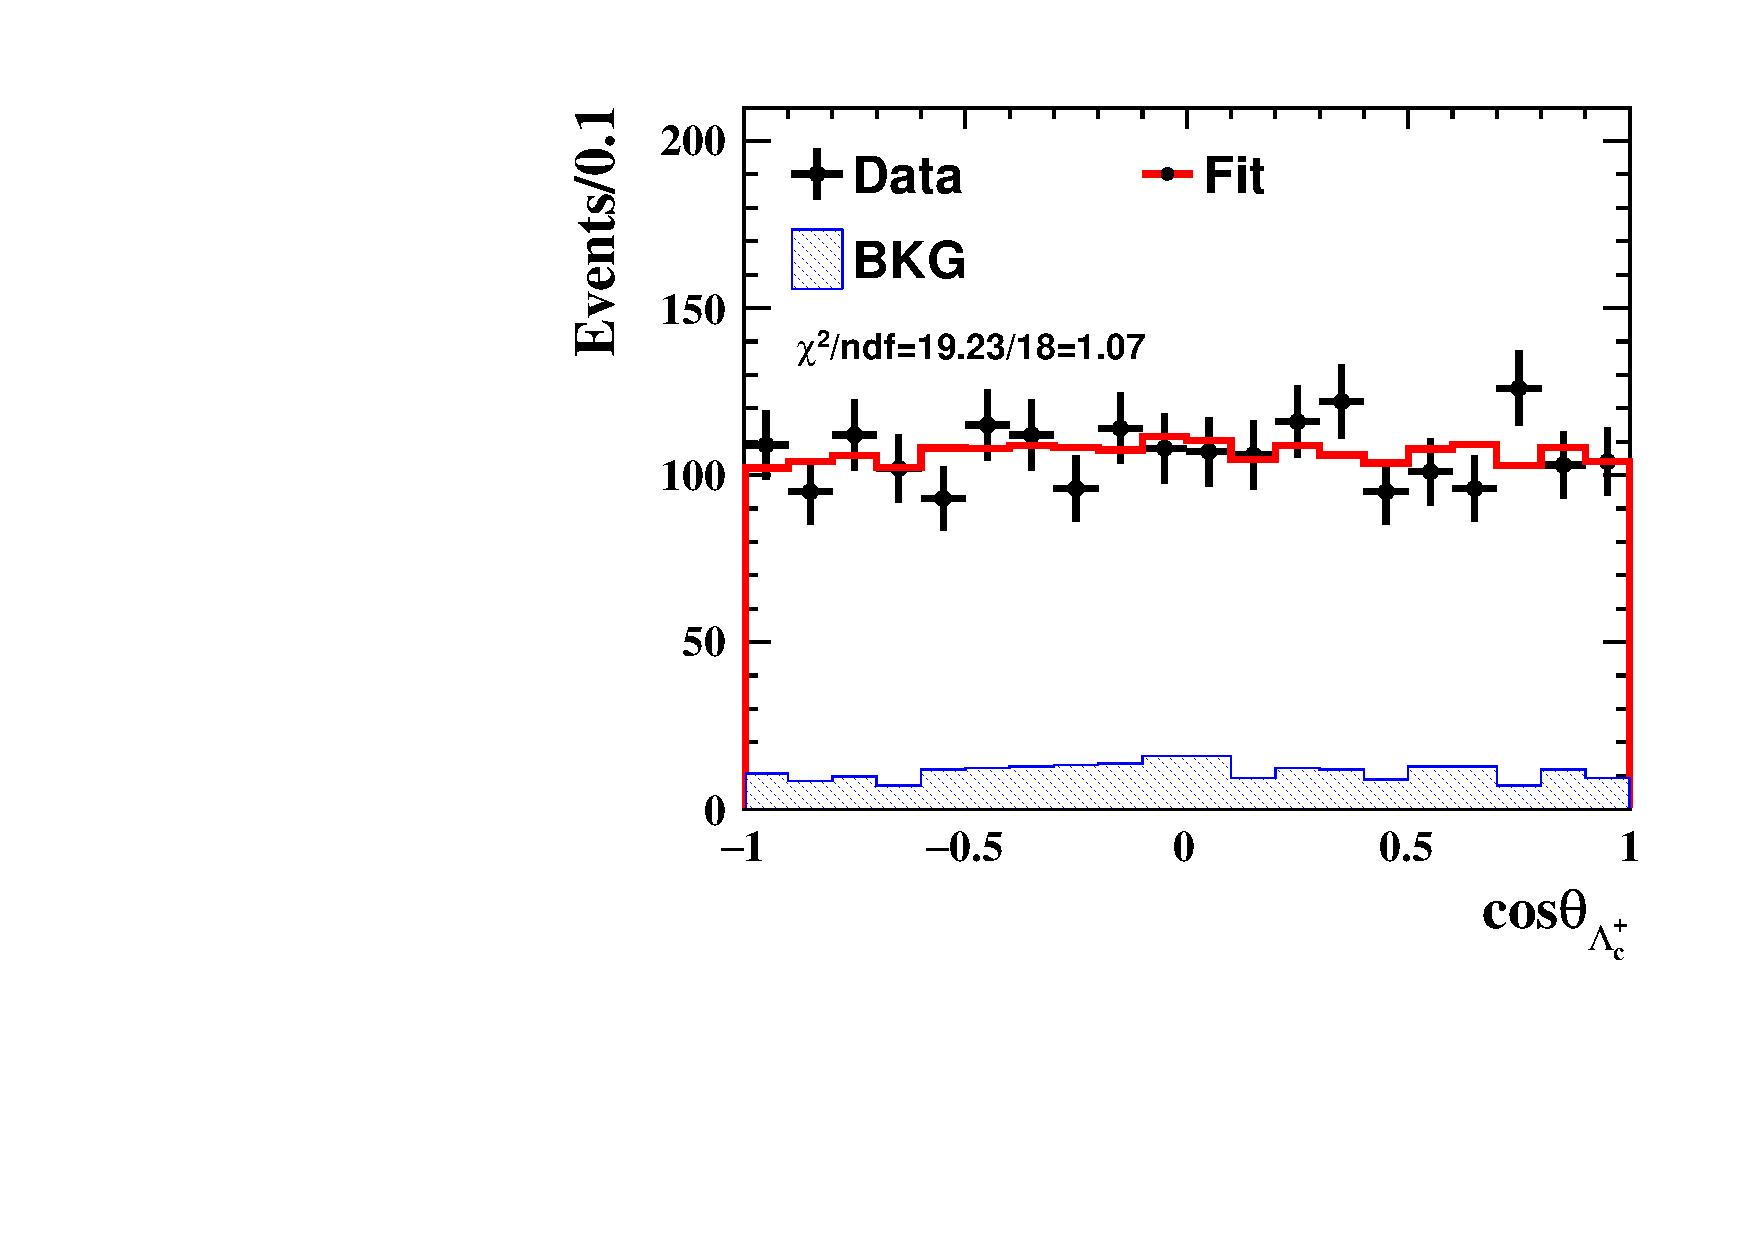
\includegraphics[width=0.24\textwidth]{figure/polarimetery/angular_plots/pkpi_4840_cos_theta0.pdf}
    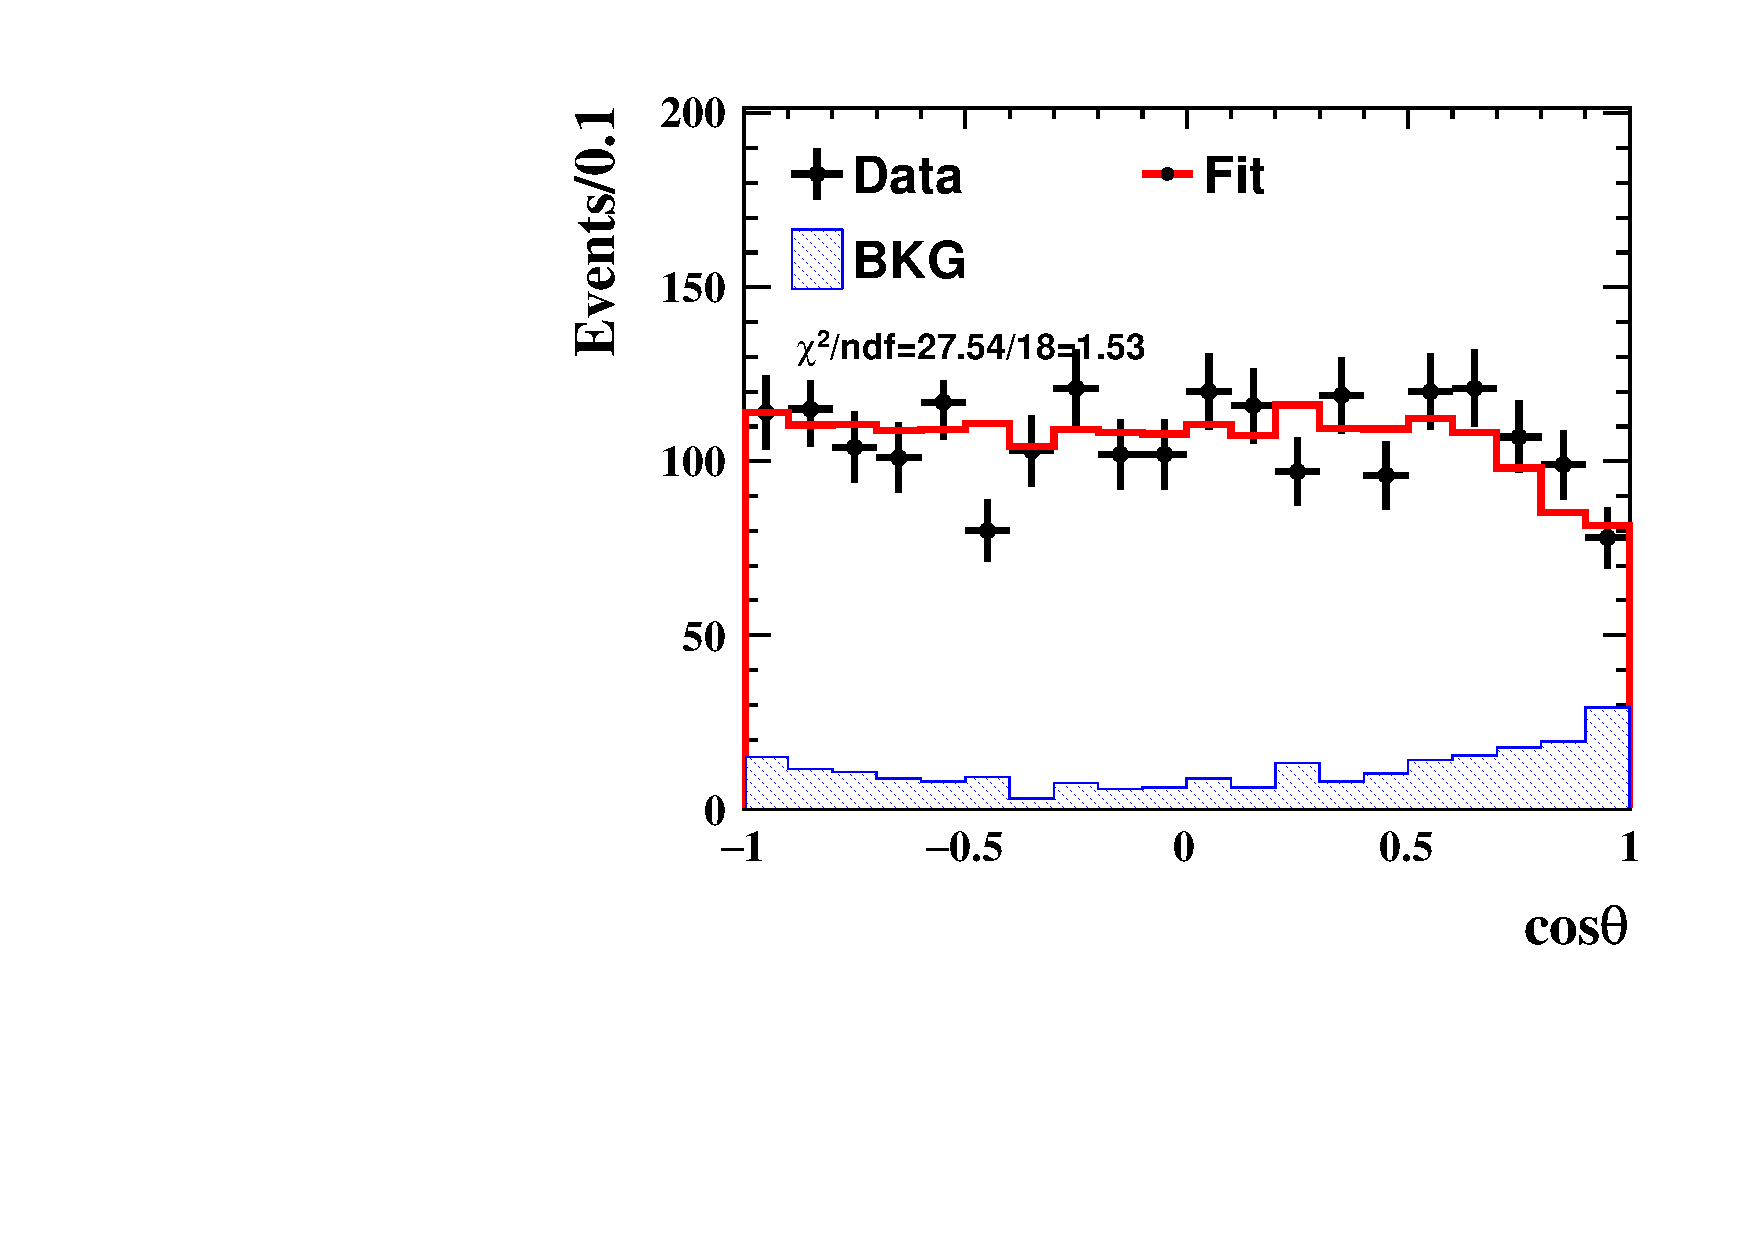
\includegraphics[width=0.24\textwidth]{figure/polarimetery/angular_plots/pkpi_4840_cos_theta1.pdf}
    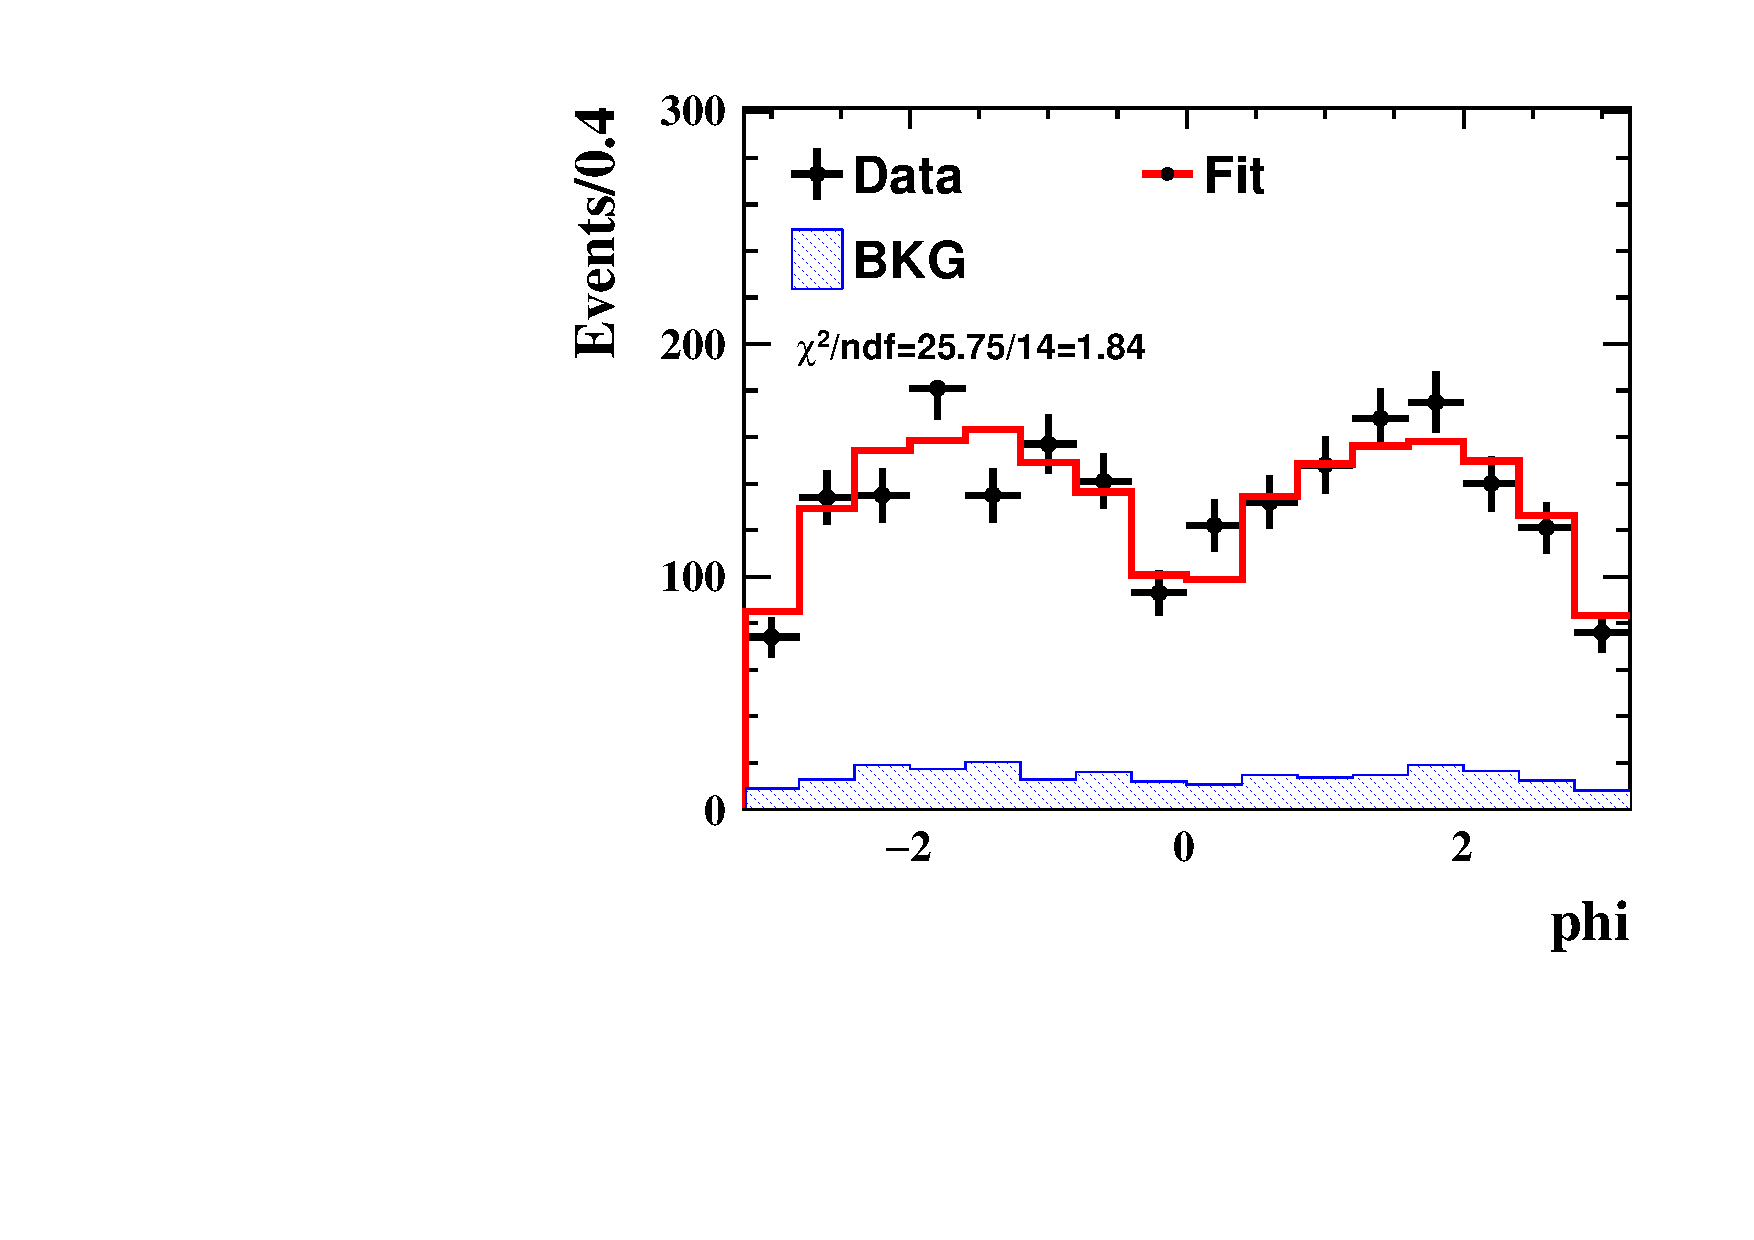
\includegraphics[width=0.24\textwidth]{figure/polarimetery/angular_plots/pkpi_4840_phi1.pdf}
    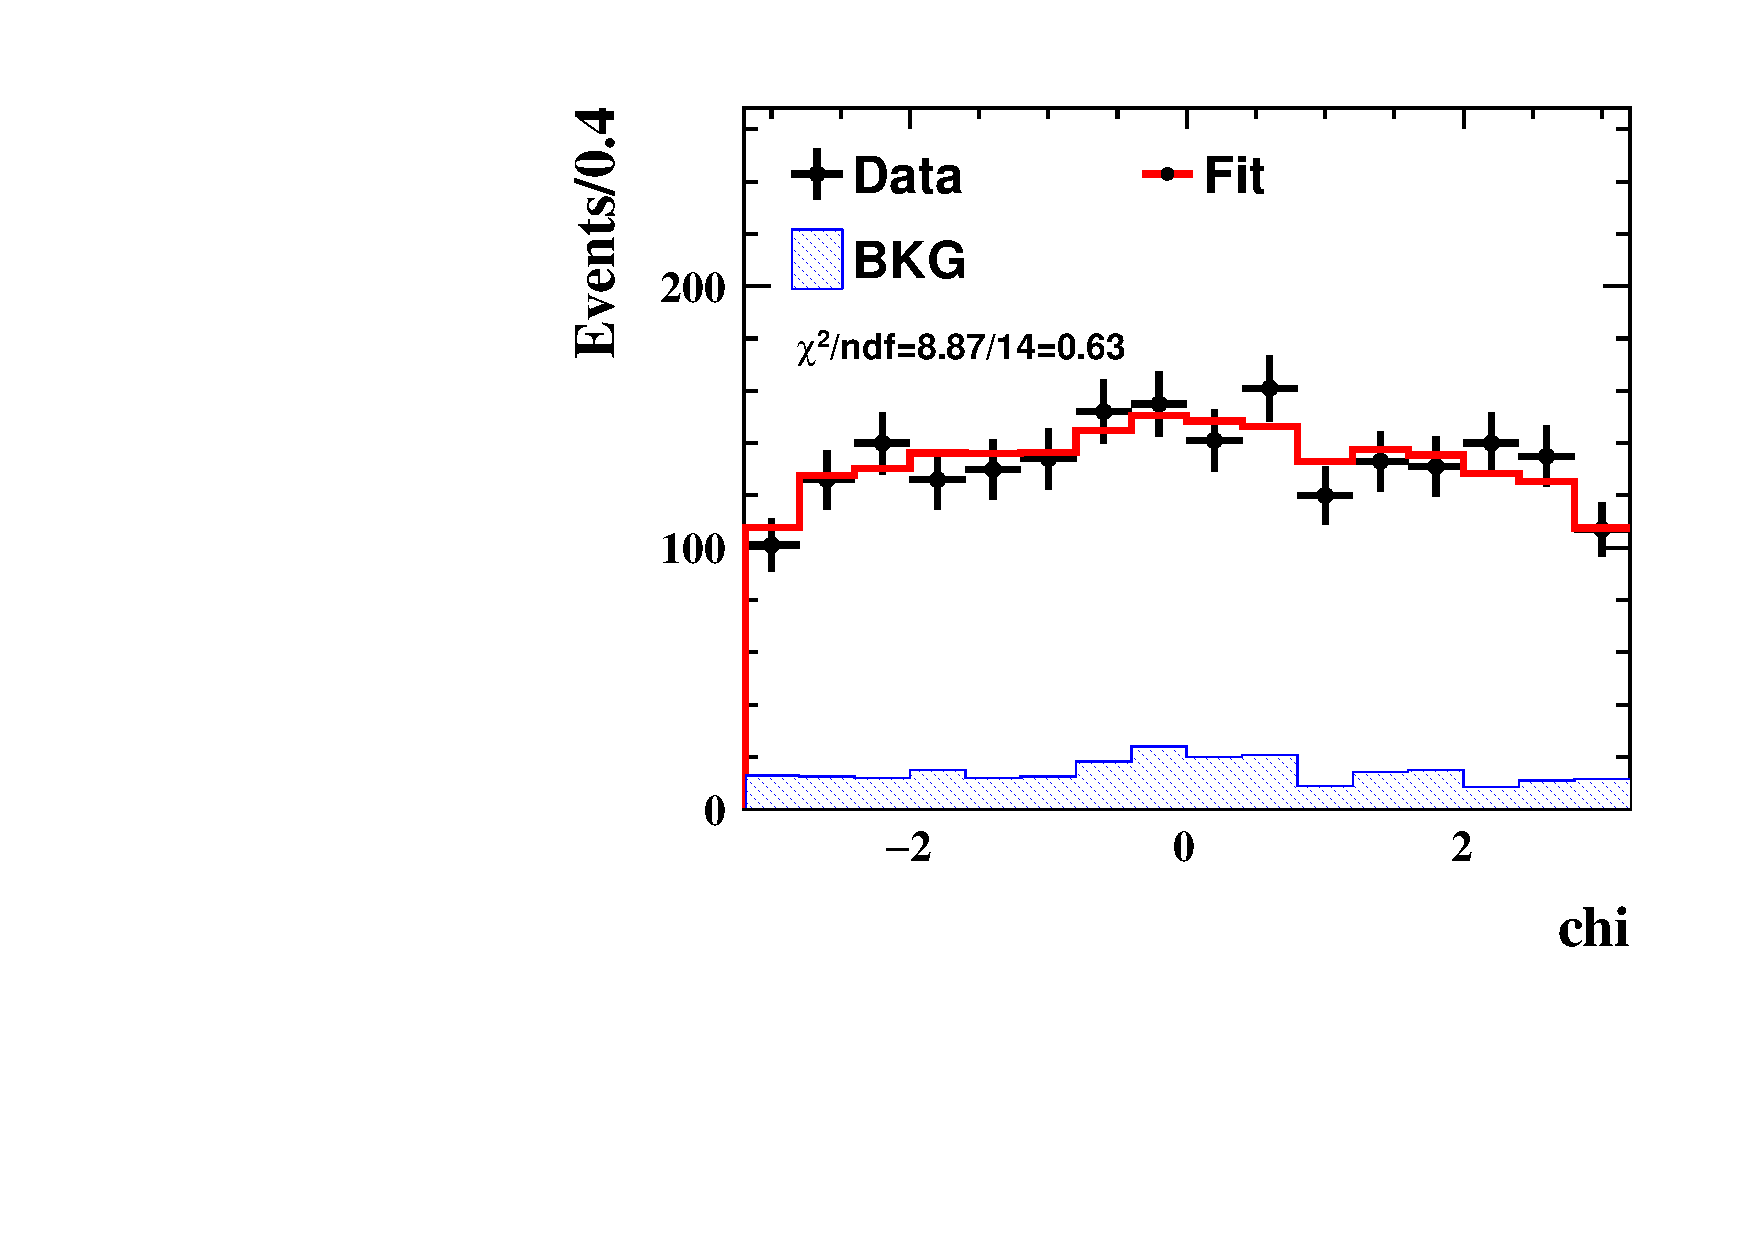
\includegraphics[width=0.24\textwidth]{figure/polarimetery/angular_plots/pkpi_4840_phi2.pdf}
    \caption{Fit results of helicity angles of $\theta_{\lcp}$, $\theta$, $\phi$ and $\chi$ at $\sqrt{s} = 4.843\gev/c^2$.}
\label{fig:fit_angular_s10}
\end{figure}

\begin{figure}[H]\centering
    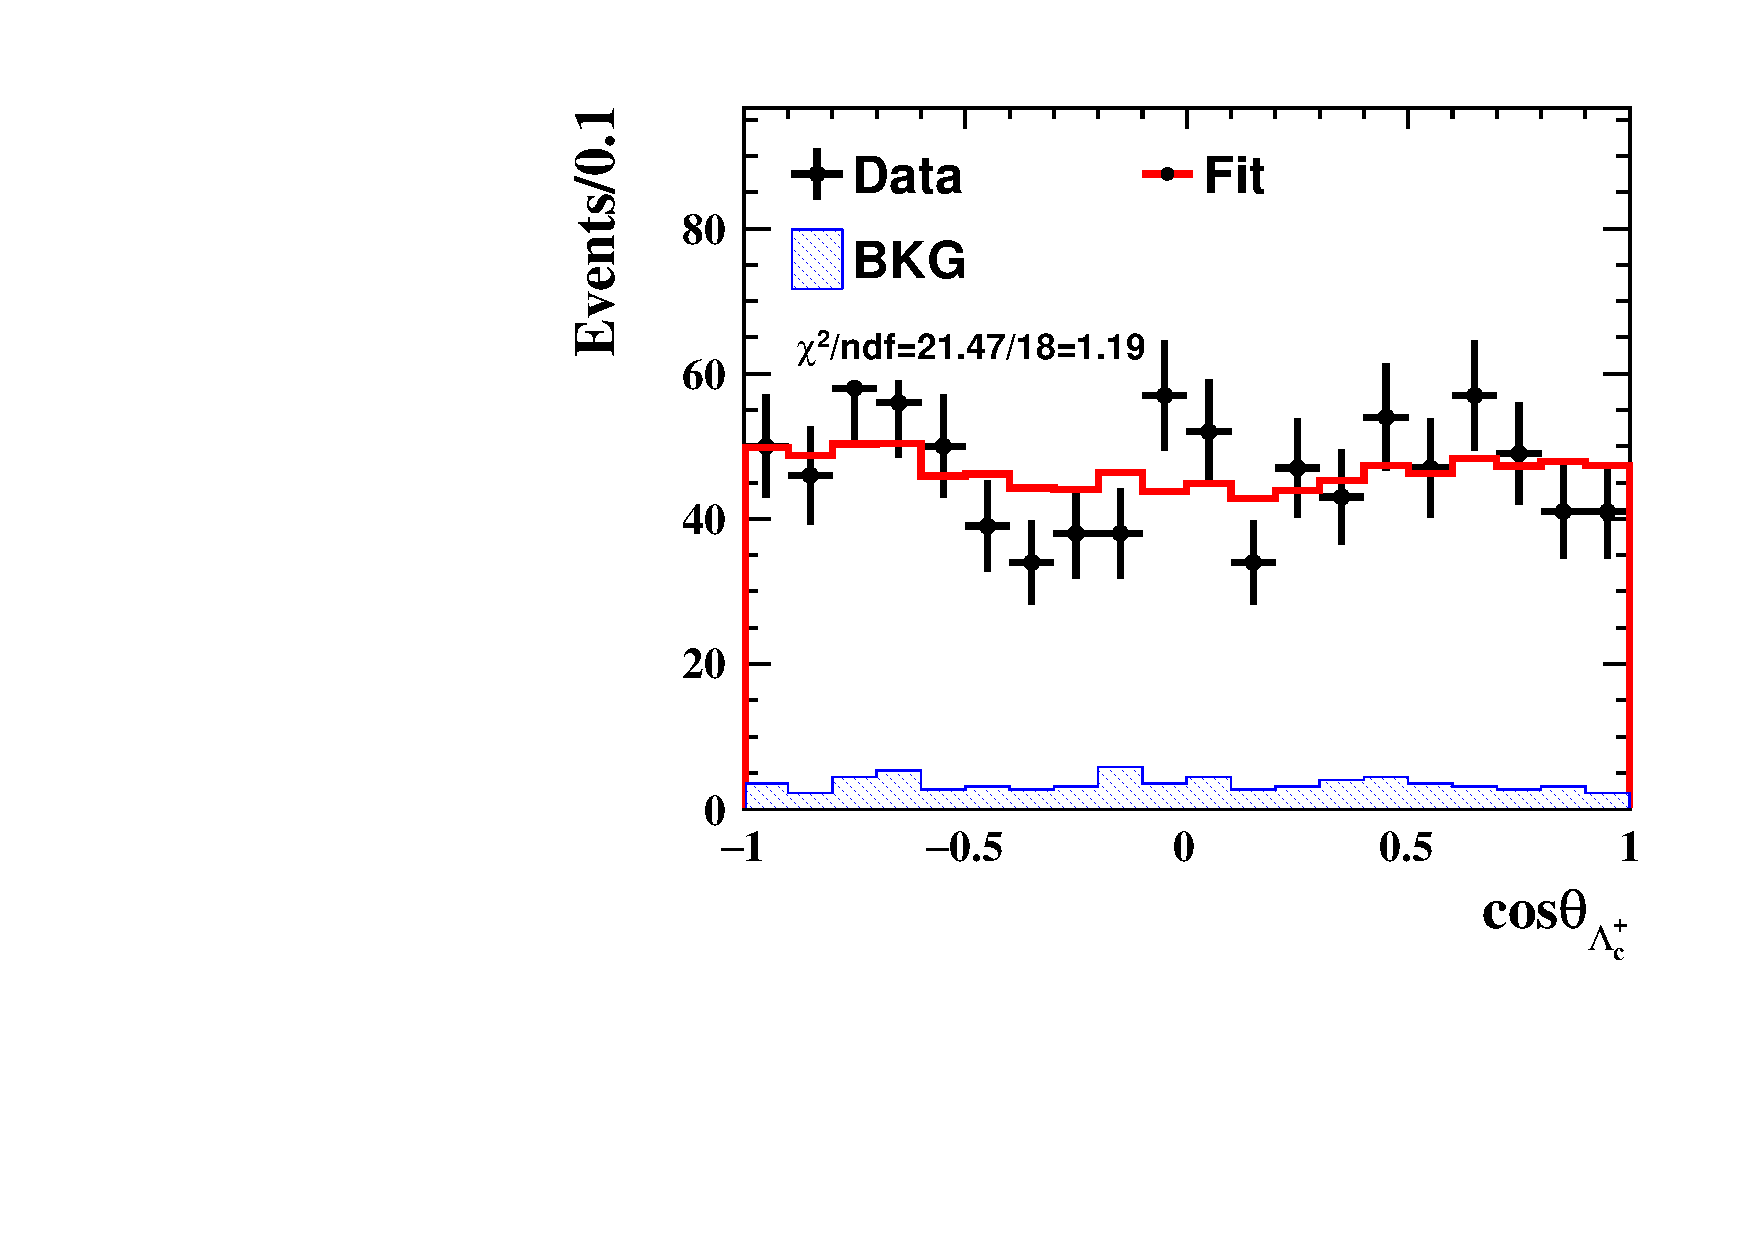
\includegraphics[width=0.24\textwidth]{figure/polarimetery/angular_plots/pkpi_4914_cos_theta0.pdf}
    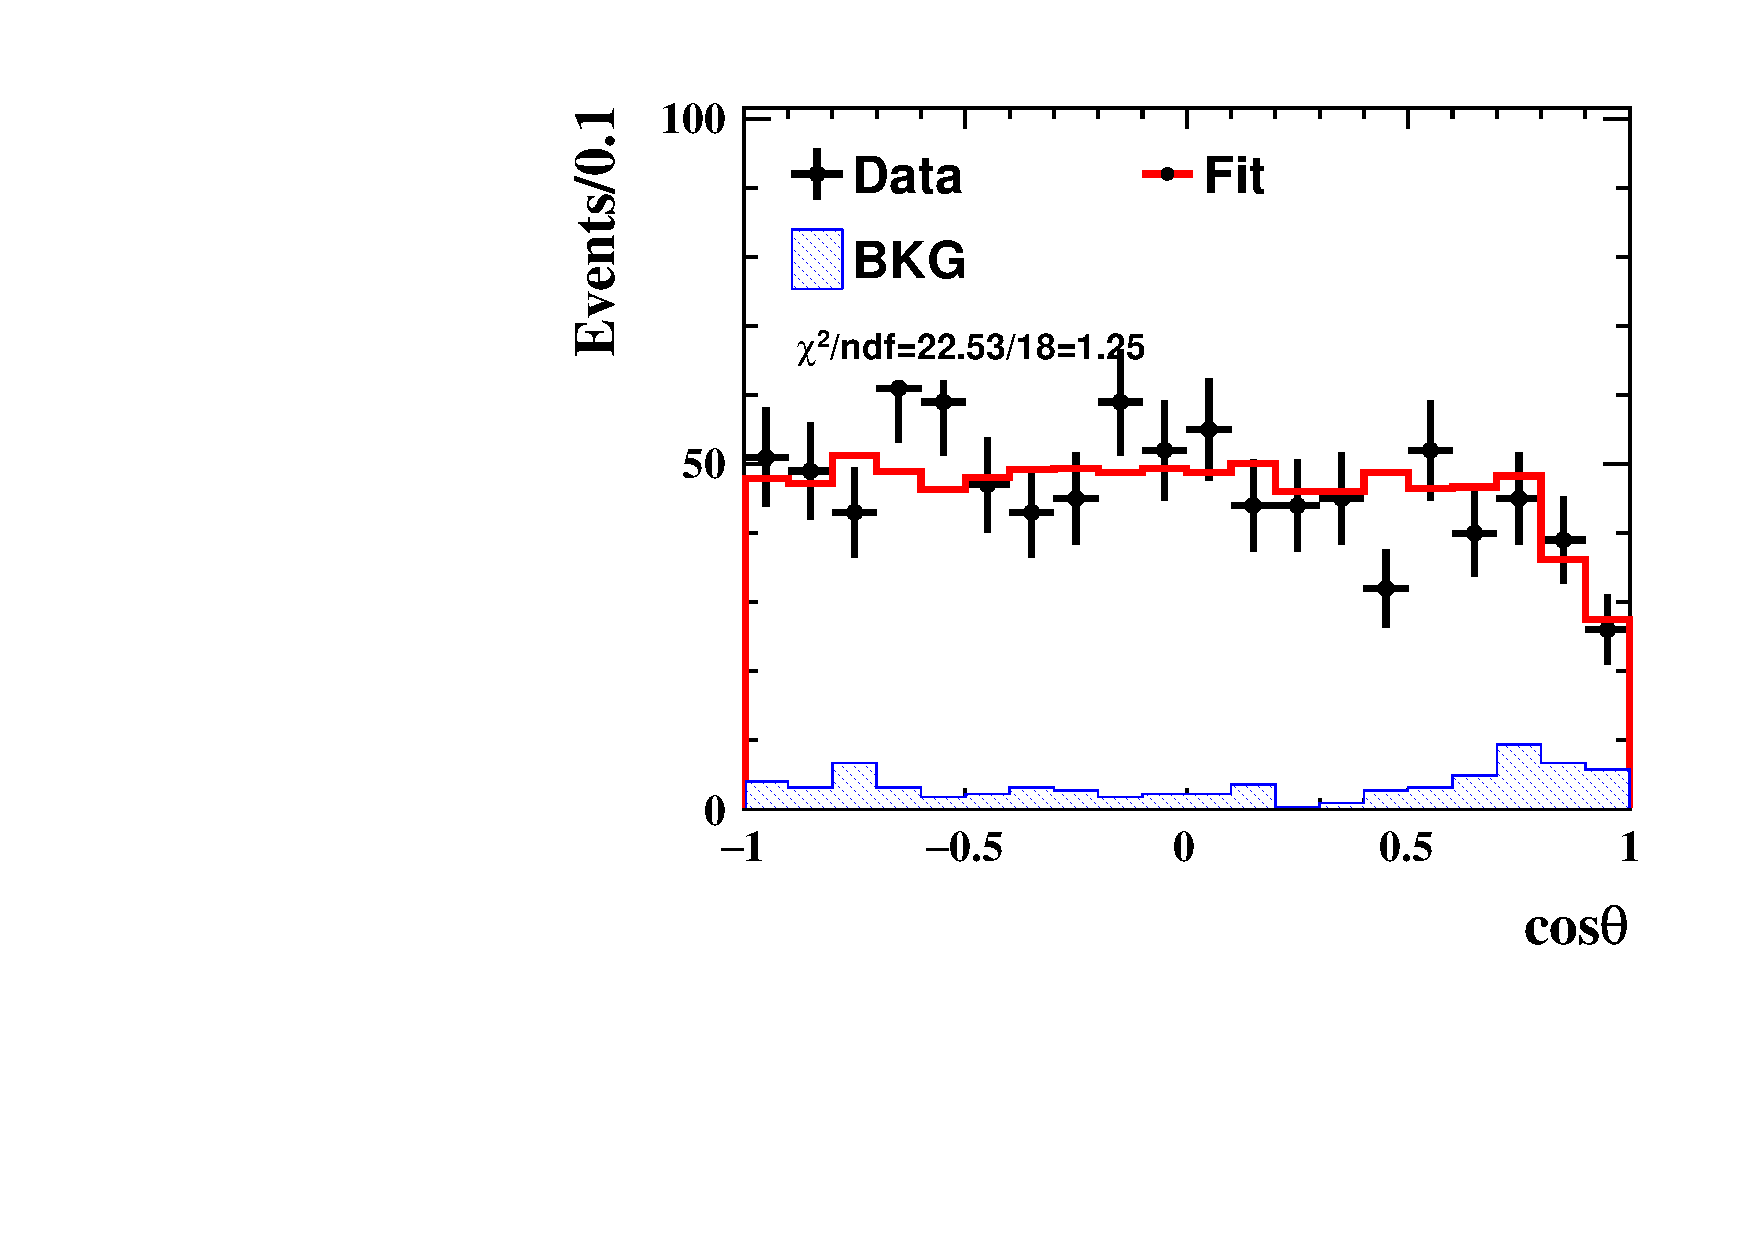
\includegraphics[width=0.24\textwidth]{figure/polarimetery/angular_plots/pkpi_4914_cos_theta1.pdf}
    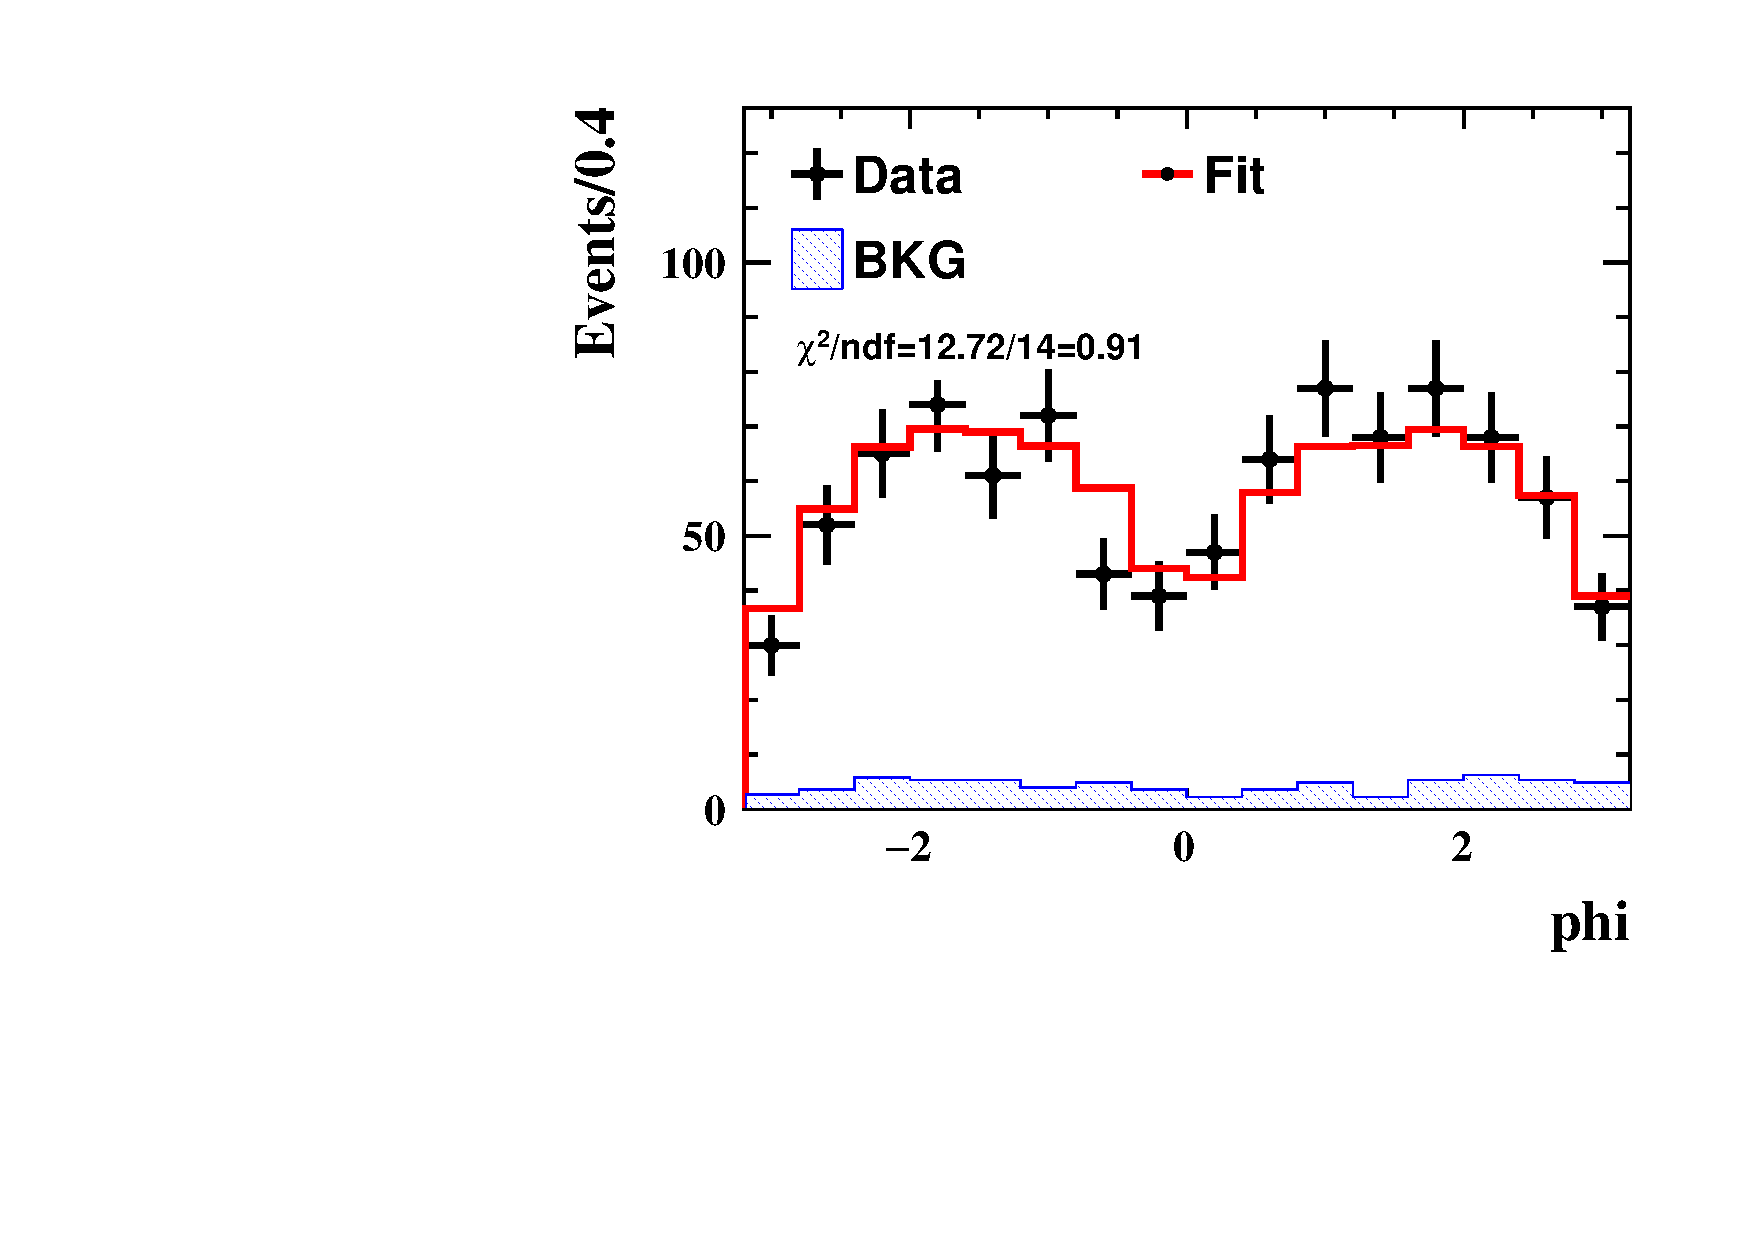
\includegraphics[width=0.24\textwidth]{figure/polarimetery/angular_plots/pkpi_4914_phi1.pdf}
    \includegraphics[width=0.24\textwidth]{figure/polarimetery/angular_plots/pkpi_4914_phi2.pdf}
    \caption{Fit results of helicity angles of $\theta_{\lcp}$, $\theta$, $\phi$ and $\chi$ at $\sqrt{s} = 4.918\gev/c^2$.}
\label{fig:fit_angular_s11}
\end{figure}

\begin{figure}[H]\centering
    \includegraphics[width=0.24\textwidth]{figure/polarimetery/angular_plots/pkpi_4946_cos_theta0.pdf}
    \includegraphics[width=0.24\textwidth]{figure/polarimetery/angular_plots/pkpi_4946_cos_theta1.pdf}
    \includegraphics[width=0.24\textwidth]{figure/polarimetery/angular_plots/pkpi_4946_phi1.pdf}
    \includegraphics[width=0.24\textwidth]{figure/polarimetery/angular_plots/pkpi_4946_phi2.pdf}
    \caption{Fit results of helicity angles of $\theta_{\lcp}$, $\theta$, $\phi$ and $\chi$ at $\sqrt{s} = 4.951\gev/c^2$.}
\label{fig:fit_angular_s12}
\end{figure}

\begin{table}[H]
\centering
\caption{Comparison of fitted $\alpha_0$ and $\sin\Delta_0$ from the amplitude analysis results and angular fit analysis. The first uncertainty is statistical uncertainty and the second one is systematic uncertainty.}
\label{tab:angular-fit}
\resizebox{\textwidth}{!}{
\begin{tabular}{c|cc|cc|cc}
\hline\hline
& \multicolumn{2}{c}{Amplitude analysis results} & \multicolumn{2}{c}{Angular fit results} & \multicolumn{2}{c}{Deviation} \\\hline
dataset & $\alpha_0$ & $\sin\Delta_0$ & $\alpha_0$ & $\sin\Delta_0$ & $\alpha_0$ ($\sigma$) & $\sin\Delta_0$ ($\sigma$)\\\hline
4600 & -0.249 $\pm$ 0.036 $\pm$ 0.002 & -0.224 $\pm$ 0.084 $\pm$ 0.059 & -0.241 $\pm$ 0.036 $\pm$ 0.001 & -0.158 $\pm$ 0.084 $\pm$ 0.014 & 0.2 & 0.5\\
4612 & -0.243 $\pm$ 0.092 $\pm$ 0.003 & -0.463 $\pm$ 0.211 $\pm$ 0.107 & -0.243 $\pm$ 0.092 $\pm$ 0.002 & -0.285 $\pm$ 0.214 $\pm$ 0.041 & 0.0 & 0.6\\
4626 & -0.191 $\pm$ 0.042 $\pm$ 0.005 & -0.244 $\pm$ 0.099 $\pm$ 0.079 & -0.178 $\pm$ 0.043 $\pm$ 0.001 & -0.283 $\pm$ 0.097 $\pm$ 0.025 & 0.2 & 0.2\\
4640 & -0.083 $\pm$ 0.045 $\pm$ 0.002 & -0.438 $\pm$ 0.096 $\pm$ 0.115 & -0.080 $\pm$ 0.045 $\pm$ 0.002 & -0.349 $\pm$ 0.095 $\pm$ 0.027 & 0.0 & 0.5\\
4660 & -0.009 $\pm$ 0.050 $\pm$ 0.004 & -0.515 $\pm$ 0.099 $\pm$ 0.039 & -0.012 $\pm$ 0.050 $\pm$ 0.001 & -0.528 $\pm$ 0.100 $\pm$ 0.021 & 0.0 & 0.1\\
4680 & 0.116 $\pm$ 0.032 $\pm$ 0.003 & -0.425 $\pm$ 0.064 $\pm$ 0.041 & 0.120 $\pm$ 0.033 $\pm$ 0.003 & -0.432 $\pm$ 0.064 $\pm$ 0.011 & 0.1 & 0.1\\
4700 & 0.318 $\pm$ 0.069 $\pm$ 0.004 & -0.585 $\pm$ 0.135 $\pm$ 0.084 & 0.317 $\pm$ 0.069 $\pm$ 0.003 & -0.564 $\pm$ 0.135 $\pm$ 0.026 & 0.0 & 0.1\\
4740 & 0.421 $\pm$ 0.159 $\pm$ 0.014 & 0.281 $\pm$ 0.298 $\pm$ 0.151 & 0.403 $\pm$ 0.157 $\pm$ 0.005 & 0.312 $\pm$ 0.296 $\pm$ 0.063 & 0.1 & 0.1\\
4750 & 0.421 $\pm$ 0.104 $\pm$ 0.007 & -0.424 $\pm$ 0.210 $\pm$ 0.152 & 0.401 $\pm$ 0.103 $\pm$ 0.002 & -0.542 $\pm$ 0.198 $\pm$ 0.043 & 0.1 & 0.4\\
4780 & 0.167 $\pm$ 0.077 $\pm$ 0.006 & -0.433 $\pm$ 0.149 $\pm$ 0.077 & 0.179 $\pm$ 0.077 $\pm$ 0.005 & -0.433 $\pm$ 0.149 $\pm$ 0.026 & 0.1 & 0.0\\
4840 & 0.334 $\pm$ 0.107 $\pm$ 0.008 & -0.429 $\pm$ 0.217 $\pm$ 0.171 & 0.333 $\pm$ 0.106 $\pm$ 0.009 & -0.343 $\pm$ 0.212 $\pm$ 0.083 & 0.0 & 0.2\\
4920 & 0.697 $\pm$ 0.196 $\pm$ 0.040 & 0.351 $\pm$ 0.446 $\pm$ 0.271 & 0.669 $\pm$ 0.191 $\pm$ 0.009 & -0.197 $\pm$ 0.417 $\pm$ 0.040 & 0.1 & 0.8\\
4950 & 0.447 $\pm$ 0.215 $\pm$ 0.027 & -0.223 $\pm$ 0.405 $\pm$ 0.400 & 0.446 $\pm$ 0.213 $\pm$ 0.012 & -0.045 $\pm$ 0.386 $\pm$ 0.073 & 0.0 & 0.3\\
\hline\hline
\end{tabular}
}
\end{table}

For the studies of systematic uncertainties, we consider the sources from the $\lcp$ polarimeter vector field provided by LHCb. The variations include statistical uncertainties from data and model uncertainties. In Ref~\cite{LHCb:2023crj}, the statistical uncertainties are estimated by varying the parameter values in the default model. These parameters are sampled by a Gaussian function, whose $\mu$ and $\sigma$ are given by the central and error values from the default model fit results in Ref~\cite{LHCb:2022ouv}. The polarimeter vector fields are reproduced for each varied parameter set. The angular fit procedure is repeated using the corresponding inputs and the statistical component is given by taken the standard deviations of the fit results. The residual distributions are shown in Figure~\ref{fig:angular_stat_alpha0} and Figure~\ref{fig:angular_stat_delta0} for $\alpha_0$ and $\sin\Delta_0$, respectively. The model uncertainties are computed using the alternative models in Ref~\cite{LHCb:2022ouv}. With alternative polarimeter field inputs, the angular fit is repeated and the maximal deviation are assigned to the model uncertainties. 
The residual distributions are shown in Figure~\ref{fig:angular_model_alpha0} and \ref{fig:angular_model_delta0}.
The systematic uncertainties from Data-MC differences and background descriptions are estimated using the same strategies documented in Section~\ref{sec:systmeatic}. The combined systematic uncertainties are listed in Table~\ref{tab:angular-fit}.

\begin{figure}[h]\centering
    \includegraphics[width=0.24\textwidth]{figure/polarimetery/syst/bootstrap/output_stat_4600_alpha0.pdf}
    \includegraphics[width=0.24\textwidth]{figure/polarimetery/syst/bootstrap/output_stat_4612_alpha0.pdf}
    \includegraphics[width=0.24\textwidth]{figure/polarimetery/syst/bootstrap/output_stat_4626_alpha0.pdf}
    \includegraphics[width=0.24\textwidth]{figure/polarimetery/syst/bootstrap/output_stat_4640_alpha0.pdf}
    \includegraphics[width=0.24\textwidth]{figure/polarimetery/syst/bootstrap/output_stat_4660_alpha0.pdf}
    \includegraphics[width=0.24\textwidth]{figure/polarimetery/syst/bootstrap/output_stat_4680_alpha0.pdf}
    \includegraphics[width=0.24\textwidth]{figure/polarimetery/syst/bootstrap/output_stat_4700_alpha0.pdf}
    \includegraphics[width=0.24\textwidth]{figure/polarimetery/syst/bootstrap/output_stat_4740_alpha0.pdf}
    \includegraphics[width=0.24\textwidth]{figure/polarimetery/syst/bootstrap/output_stat_4750_alpha0.pdf}
    \includegraphics[width=0.24\textwidth]{figure/polarimetery/syst/bootstrap/output_stat_4780_alpha0.pdf}
    \includegraphics[width=0.24\textwidth]{figure/polarimetery/syst/bootstrap/output_stat_4840_alpha0.pdf}
    \includegraphics[width=0.24\textwidth]{figure/polarimetery/syst/bootstrap/output_stat_4920_alpha0.pdf}
    \includegraphics[width=0.24\textwidth]{figure/polarimetery/syst/bootstrap/output_stat_4950_alpha0.pdf}
    \caption{Distributions of residual for $\alpha_0$ for statistical components}
\label{fig:angular_stat_alpha0}
\end{figure}

\begin{figure}[h]\centering
    \includegraphics[width=0.24\textwidth]{figure/polarimetery/syst/bootstrap/output_stat_4600_delta0.pdf}
    \includegraphics[width=0.24\textwidth]{figure/polarimetery/syst/bootstrap/output_stat_4612_delta0.pdf}
    \includegraphics[width=0.24\textwidth]{figure/polarimetery/syst/bootstrap/output_stat_4626_delta0.pdf}
    \includegraphics[width=0.24\textwidth]{figure/polarimetery/syst/bootstrap/output_stat_4640_delta0.pdf}
    \includegraphics[width=0.24\textwidth]{figure/polarimetery/syst/bootstrap/output_stat_4660_delta0.pdf}
    \includegraphics[width=0.24\textwidth]{figure/polarimetery/syst/bootstrap/output_stat_4680_delta0.pdf}
    \includegraphics[width=0.24\textwidth]{figure/polarimetery/syst/bootstrap/output_stat_4700_delta0.pdf}
    \includegraphics[width=0.24\textwidth]{figure/polarimetery/syst/bootstrap/output_stat_4740_delta0.pdf}
    \includegraphics[width=0.24\textwidth]{figure/polarimetery/syst/bootstrap/output_stat_4750_delta0.pdf}
    \includegraphics[width=0.24\textwidth]{figure/polarimetery/syst/bootstrap/output_stat_4780_delta0.pdf}
    \includegraphics[width=0.24\textwidth]{figure/polarimetery/syst/bootstrap/output_stat_4840_delta0.pdf}
    \includegraphics[width=0.24\textwidth]{figure/polarimetery/syst/bootstrap/output_stat_4920_delta0.pdf}
    \includegraphics[width=0.24\textwidth]{figure/polarimetery/syst/bootstrap/output_stat_4950_delta0.pdf}
    \caption{Distributions of residual for $\Delta_0$ for statistical components}
\label{fig:angular_stat_delta0}
\end{figure}

\begin{figure}[h]\centering
    \includegraphics[width=0.24\textwidth]{figure/polarimetery/syst/model/output_model_4600_alpha0.pdf}
    \includegraphics[width=0.24\textwidth]{figure/polarimetery/syst/model/output_model_4612_alpha0.pdf}
    \includegraphics[width=0.24\textwidth]{figure/polarimetery/syst/model/output_model_4626_alpha0.pdf}
    \includegraphics[width=0.24\textwidth]{figure/polarimetery/syst/model/output_model_4640_alpha0.pdf}
    \includegraphics[width=0.24\textwidth]{figure/polarimetery/syst/model/output_model_4660_alpha0.pdf}
    \includegraphics[width=0.24\textwidth]{figure/polarimetery/syst/model/output_model_4680_alpha0.pdf}
    \includegraphics[width=0.24\textwidth]{figure/polarimetery/syst/model/output_model_4700_alpha0.pdf}
    \includegraphics[width=0.24\textwidth]{figure/polarimetery/syst/model/output_model_4740_alpha0.pdf}
    \includegraphics[width=0.24\textwidth]{figure/polarimetery/syst/model/output_model_4750_alpha0.pdf}
    \includegraphics[width=0.24\textwidth]{figure/polarimetery/syst/model/output_model_4780_alpha0.pdf}
    \includegraphics[width=0.24\textwidth]{figure/polarimetery/syst/model/output_model_4840_alpha0.pdf}
    \includegraphics[width=0.24\textwidth]{figure/polarimetery/syst/model/output_model_4920_alpha0.pdf}
    \includegraphics[width=0.24\textwidth]{figure/polarimetery/syst/model/output_model_4950_alpha0.pdf}
    \caption{Distributions of residual for $\alpha_0$ for model components}
\label{fig:angular_model_alpha0}
\end{figure}

\begin{figure}[h]\centering
    \includegraphics[width=0.24\textwidth]{figure/polarimetery/syst/model/output_model_4600_delta0.pdf}
    \includegraphics[width=0.24\textwidth]{figure/polarimetery/syst/model/output_model_4612_delta0.pdf}
    \includegraphics[width=0.24\textwidth]{figure/polarimetery/syst/model/output_model_4626_delta0.pdf}
    \includegraphics[width=0.24\textwidth]{figure/polarimetery/syst/model/output_model_4640_delta0.pdf}
    \includegraphics[width=0.24\textwidth]{figure/polarimetery/syst/model/output_model_4660_delta0.pdf}
    \includegraphics[width=0.24\textwidth]{figure/polarimetery/syst/model/output_model_4680_delta0.pdf}
    \includegraphics[width=0.24\textwidth]{figure/polarimetery/syst/model/output_model_4700_delta0.pdf}
    \includegraphics[width=0.24\textwidth]{figure/polarimetery/syst/model/output_model_4740_delta0.pdf}
    \includegraphics[width=0.24\textwidth]{figure/polarimetery/syst/model/output_model_4750_delta0.pdf}
    \includegraphics[width=0.24\textwidth]{figure/polarimetery/syst/model/output_model_4780_delta0.pdf}
    \includegraphics[width=0.24\textwidth]{figure/polarimetery/syst/model/output_model_4840_delta0.pdf}
    \includegraphics[width=0.24\textwidth]{figure/polarimetery/syst/model/output_model_4920_delta0.pdf}
    \includegraphics[width=0.24\textwidth]{figure/polarimetery/syst/model/output_model_4950_delta0.pdf}
    \caption{Distributions of residual for $\Delta_0$ for model components}
\label{fig:angular_model_delta0}
\end{figure}
